\documentclass[a4paper,12pt,italian,twoside]{book}
\usepackage[italian]{babel}
\usepackage[utf8]{inputenc}
\usepackage{amssymb}
\usepackage{amsmath}
\usepackage{graphicx}
\usepackage{enumerate}
\usepackage{fancyhdr}
\usepackage[labelfont=bf]{caption}
\usepackage{minitoc}
\usepackage[binding=1.5cm]{layaureo}
\usepackage{threeparttable}
\usepackage{booktabs}
\usepackage{longtable}
\usepackage{multirow}
\usepackage{array}
\usepackage{color}
\usepackage{comment}
\usepackage{ulem}\normalem
\usepackage{textcomp}
\usepackage[perpage,symbol*]{footmisc}
\usepackage{epstopdf}
\usepackage{csquotes}

\usepackage[style=ieee, backend=biber, citestyle=numeric-comp]{biblatex}
\addbibresource{./bibliografia/Th.bib}
\addbibresource{./bibliografia/Th-Adapt.bib}

\hyphenation{MATLAB}
\hyphenation{IMRT}
\hyphenation{VMAT}
\newcommand{\virg}[1]{\textquotedblleft \emph{#1}\textquotedblright{}}
\newcommand{\virgbf}[1]{\textquotedblleft \textbf{\emph{#1}}\textquotedblright{}}
\newcommand{\de}{\,\text{d}}
\newcommand{\RS}{RayStation\textsuperscript{\textcopyright}}
\newcommand{\arrstr}[1]{\renewcommand{\arraystretch}{#1}}

\setcounter{tocdepth}{3}
\setcounter{secnumdepth}{3}  %Per avere le subsubsection numerate

%%%%%%AMBIENTE ABSTRACT%%%%%%%
%\newcommand{\abstractmodificato}[1]{
%
%\vspace*{3cm}
%\begin{center}
%
%\textbf{Abstract\\}
%\begin{minipage}[t]{0.7\columnwidth}
%
%\begin{small}{#1}\end{small}
%
%\end{minipage}
%
%\end{center}
%} 


%%%%%%INTESTAZIONE ELEGANTE%%%%%%
\pagestyle{fancy}
% with this we ensure that the chapter and section
% headings are in lowercase.
\renewcommand{\chaptermark}[1]{%
\markboth{#1}{}}
\renewcommand{\sectionmark}[1]{%
\markright{\thesection\ #1}}
\fancyhf{} % delete current header and footer
\fancyhead[LE,RO]{\bfseries\thepage}
\fancyhead[LO]{\bfseries\rightmark}
\fancyhead[RE]{\bfseries\leftmark}
\renewcommand{\headrulewidth}{0.5pt}
\renewcommand{\footrulewidth}{0pt}
\addtolength{\headheight}{2.5pt} % space for the rule
\fancypagestyle{plain}{%
\fancyhead{} % get rid of headers on plain pages
\renewcommand{\headrulewidth}{0pt} }
%%%%%%INTESTAZIONE ELEGANTE%%%%%%

%%%%%%INIZIO DOCUMENTO%%%%%%
\begin{document}
\dominitoc % Initialization minitocs
  
\frontmatter
%%%%%%FORNTESPIZIO%%%%%%
\begin{titlepage}
\pagestyle{empty}
\begingroup
% INTESTAZIONE
\vspace*{-7\topskip}

%%%%%%%%%%%%%%%%%%%%%%%%%%%%%%%%%%%%%%%%%%%%%%%%%%%%
%  FIGURA!!!!%%%%%%%%%%%%%%%%%%%%%%%%%%%%%%%%%%%%%%%
%%%%%%%%%%%%%%%%%%%%%%%%%%%%%%%%%%%%%%%%%%%%%%%%%%%%

\begin{figure}[!h]
%centrare
\begin{center}
%resize in cm

\includegraphics[scale=0.15]{frontespizio/logo_aq.jpg}

\includegraphics[scale=0.25]{frontespizio/logo_dept.jpg}
\end{center}
\end{figure}

\vspace{-1cm}

\centering \expandafter{\Large{UNIVERSIT\`{A} DEGLI STUDI DELL'AQUILA}\par}
\begin{center}
\Large{\rm\expandafter{Dipartimento di Medicina clinica, Sanità pubblica, Scienze della vita e dell'ambiente}}\\
\large\expandafter{\textbf{Scuola di Specializzazione in Fisica Medica}}
\end{center}

\vspace{0.5cm}
\begin{center}
        {\large{Tesi di Specializzazione}\par}
\end{center}

% TITOLO
\vspace{1.5cm}
\begin{center}
        {\huge\bf \baselineskip=0.95em plus 1pt \expandafter{
        Commissioning di un Sistema di elaborazione di piani di trattamento radioterapici\\\vspace{.5cm}
        \LARGE dalla 3D-CRT alla Radioterapia Adattiva}}
\end{center}





\vspace{3.5cm}

\begin{tabular}{c p{2.5 cm}c c}
\vspace{0.2cm}
Specializzando & & Relatore  \\
\vspace{0.2cm}
\large{\textbf{Alessandro Savini}} & & Dr.ssa \large{\textbf{Federica Rosica}}\\
 &&  \\
\dotfill && \dotfill \vspace{0.9cm}\\
\vspace{0.2cm}
         && Co-Relatore\\
				\vspace{0.2cm}
         && Dr. \large{\textbf{Giovanni Orlandi}}\\
&& \\
&& \dotfill

\end{tabular}
\vspace{2.5 cm}



%CHIUSURA
\begin{center}

\large{Anno Accademico 2014-2015}
\vspace{-2.5cm}
\end{center}

\clearpage
\endgroup

\end{titlepage}

\thispagestyle{empty}

%%%%%%DEDICA%%%%%%
\chapter*{}
\begin{flushright}
\emph{Alla mia Famiglia che ha permesso\\ che i miei sogni divenissero realtà.\\\vspace{.8cm} Ai miei Insegnanti che hanno contribuito\\ alla mia realizzazione umana e professionale.}
\end{flushright}
\newpage
\thispagestyle{empty}

%%%%%%PREFAZIONE%%%%%%
\chapter*{Introduzione} 
\addstarredchapter{Introduzione} %NECESSARIO PER I MINITOC SE NO SI SBALLANO
Il lavoro di tesi si è ...\cite{Mzenda2014}

\tableofcontents

%%%%%%CORPO DOCUMENTO%%%%%%
\mainmatter
\chapter{L'algoritmo \emph{collapsed cone} e la sua implementazione in RayStation}
\setcounter{minitocdepth}{1}
\minitoc
\setcounter{minitocdepth}{2}
\textsf{In questo capitolo verrà descritto l'algoritmo di calcolo dosimetrico \textit{collapsed-cone-convolution} e la sua implementazione all'interno del treatment planning system (TPS) \RS. Ci si soffermerà in particolare sugli aspetti riguardanti le approssimazioni intrinseche dell'algoritmo assieme alle approssimazioni adottate in fase di implementazione nel TPS. Ciò è propedeutico alla comprensione dei limiti e delle precisioni raggiungibili durante la modellizzazione di un fascio clinico per trattamenti radioterapici che verrà discusso nei capitoli successivi.}

\section{Introduzione}
In radioterapia la \textit{dose assorbita} è quella quantità che viene utilizzata al pari della dose farmacologica per ottenere un determinato effetto terapeutico. Più precisamente la definizione formale è fornita nel report ICRU n.85 \cite{ICRU85} come rapporto tra l'energia media $\de \bar{\varepsilon}$ impartita da radiazioni ionizzanti ad una massa $\de m$:
\begin{equation}
D = \frac{\de \bar{\varepsilon}}{\de m} \qquad\qquad \text{Unità: J\,kg}^{-1} \equiv \text{Gray [Gy]}
\end{equation} 
Esistono varie modalità di impartire una certa dose ad un paziente in radioterapia. Nell'ambito di questo lavoro si considererà solo la tecnica che fa impiego di fotoni generati da un acceleratore lineare (LINAC) denominata \virg{radioterapia a fasci esterni}.

Un LINAC è un'apparecchiatura in grado di accelerare elettroni fino ad energie dell'ordine dei 20 MeV che vanno a collidere su un target da cui si origina radiazione di frenamento (bremsstrahlung). Il fascio di fotoni così generato viene opportunamente filtrato e collimato per generare un fascio terapeutico. 
\begin{figure}
\centering
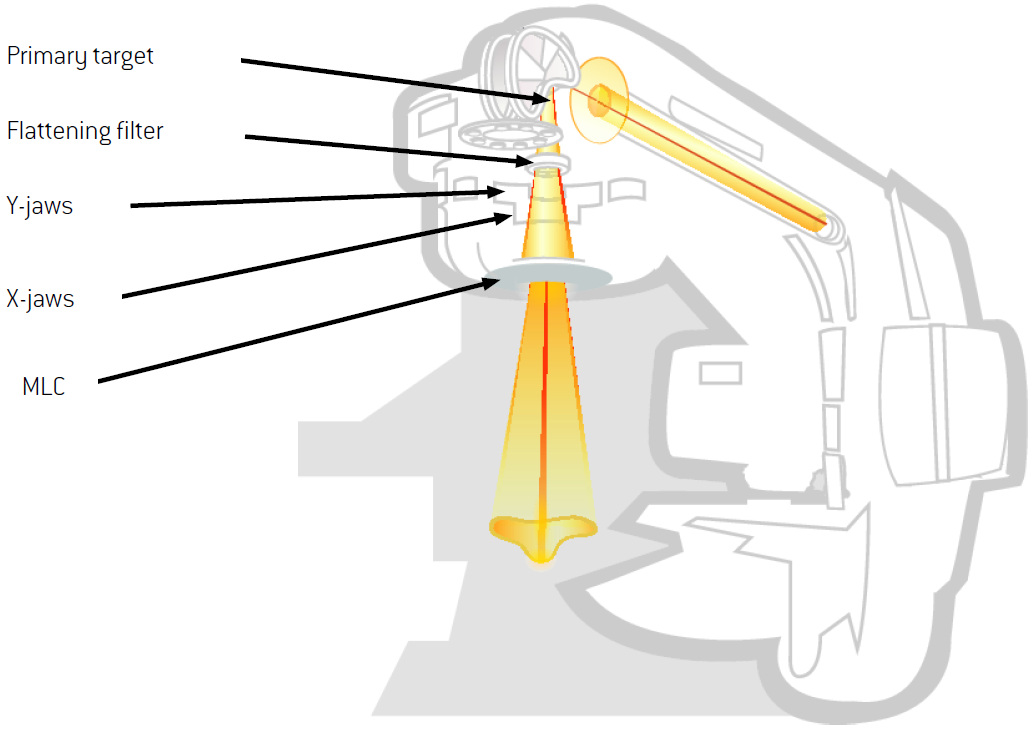
\includegraphics[width=.7\textwidth]{./cap1/linac.png}
\caption{Figura schematica di un acceleratore lineare per radioterapia a fasci esterni.}
\label{fig:linac}
\end{figure}
Tutto ciò si realizza nella testata del LINAC mediante l'uso di opportuni materiali schermanti che sono indicati nel disegno schematico riportato in Fig.\ref{fig:linac}.

Una volta che il fascio clinico investe il paziente, il meccanismo di deposizione della dose è un processo molto complesso dovuto alla grande quantità di processi che vengono innescati in cascata. \`{E} importante notare che una parte non trascurabile di processi avviene anche a livello della testata e questi vanno ad influenzare il fascio che effettivamente giunge al paziente. Ad esempio uno degli effetti più clinicamente rilevanti è la generazione di elettroni che \textquotedblleft contaminano\textquotedblright{} il fascio fotonico.

\begin{figure}
\centering
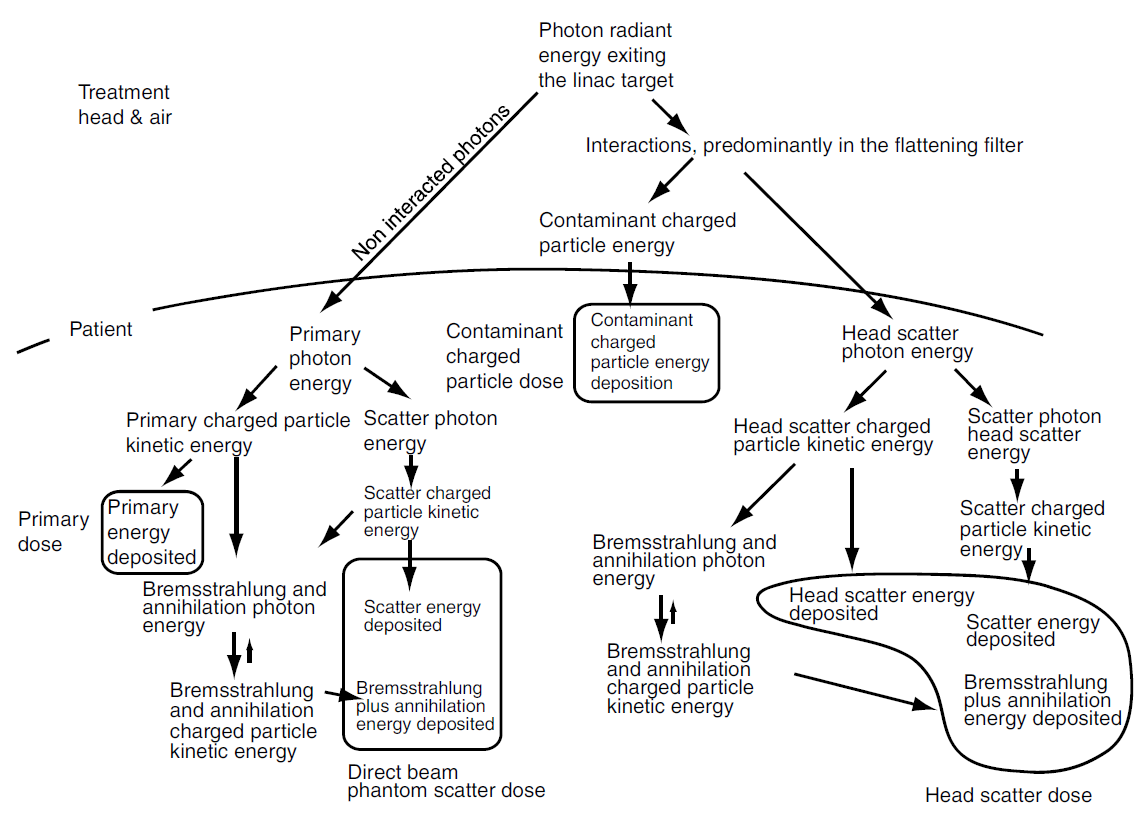
\includegraphics[width=.9\textwidth]{./cap1/processes.png}
\caption{Rappresentazione schematica delle principali interazioni che portano alla deposizione della dose nel paziente.}
\label{fig:processes}
\end{figure}
\vspace{.2cm}
La Fig.\ref{fig:processes} riassume schematicamente le principali interazioni che portano alla deposizione della dose nel paziente. \`{E} possibile identificare quattro principali meccanismi di rilascio della dose (cerchiati nella figura) che elenchiamo in ordine di importanza:
\begin{enumerate}
\item La dose primaria che rappresenta generalmente fino al 70\% della dose totale. Questa dose è generata dalla parte di fascio fotonico che non ha subito trasformazioni nella testata e che mette in moto particelle cariche le quali direttamente rilasciano la loro energia cinetica nella materia.
\item La dose di scatter dovuta al paziente (\textit{phantom scatter dose}) che può rappresentare fino al 30\% della dose totale. Questa componente è dovuta a tutti i processi di scatter che si innescano nel paziente a partire dal fascio primario come ad esempio fotoni di bremsstrahlung o fotoni scatterati per effetto Compton che portano ad una ionizzazione della materia con lo stesso meccanismo del fascio primario (messa in moto di elettroni).
\item La dose di scatter dovuta alla testata (\textit{head scatter dose}) che rappresenta generalmente il 5-10\% della dose totale. Questa parte della dose è dovuta alla componente di fascio fotonico incidente sul paziente che ha subito interazioni nella testata (prevalentemente nel \textit{flattening-filter}\footnote{Il \textit{flattening-filter} è un dispositivo di forma piramidale che serve ad attenuare il fascio al centro in modo da realizzare una fluenza di fotoni uniforme lungo la direzione perpendicolare al fascio.}) e che presenta una distribuzione spaziale ed energetica differente dal fascio primario. Il meccanismo di rilascio dell'energia è esattamente analogo a quello del fascio primario.
\item La dose dovuta alle particelle di contaminazione del fascio fotonico che hanno un effetto rilevante (comparabile con il fascio primario) soltanto nei primi centimetri di tessuto. Questa zona è conosciuta come \textit{regione di build-up} della dose e vedremo in seguito il perché.
\end{enumerate}


\section{Generalità sugli algoritmi di calcolo della dose al paziente per fasci di fotoni}
Un algoritmo di calcolo dosimetrico ha lo scopo di predire con un certo livello di accuratezza gli effetti presentati nella sezione precedente. In particolare il fine ultimo è predire la distribuzione di dose totale assorbita nel paziente che costituisce l'entità correlata all'effetto terapeutico sul tumore o al danno sul tessuto sano. La possibilità di prevedere questa quantità è propedeutica al processo noto come \textit{pianificazione del trattamento} in cui vengono adoperate delle opportune scelte riguardanti la collimazione e l'intensità del fascio volte a minimizzare il rapporto rischio/beneficio della terapia.

Esistono due grandi classi di algoritmi dosimetrici:
\begin{itemize}
\item Algoritmi \textit{correction-based}.
\item Algoritmi \textit{model-based}.
\end{itemize}
Gli algoritmi correction-based sono algoritmi empirici. Essi sono  basati su un gruppo di dati misurati in condizioni di riferimento (in un fantoccio ad acqua) e fanno uso di fattori o funzioni matematiche di tipo analitico o di tipo look-up-table per predire la distribuzione di dose assorbita in condizioni diverse da quelle di misura. 
Questi metodi furono i primi ad essere implementati in quanto non necessitano di grosse potenze di calcolo ma, d'altro canto, presentano dei limiti di accuratezza intrinseci per situazioni complesse (mezzi non omogenei, interfacce tra tessuti, campi di irradiazione molto irregolari o ad intensità modulata\ldots). Un'estensiva review di questi tipi di algoritmi è stata pubblicata da Fraass \textit{et al.}\cite{Fraass1995}.

\vspace{.2cm}
L'avvento della rivoluzione tecnologica e la crescita della potenza di calcolo disponibile tramite computer, ha permesso l'implementazione degli algoritmi model-based i quali simulano i processi di interazione radiazione-materia  a partire da principi primi tramite un modello fisico-matematico.\\
In questo caso il set di misure iniziali è unicamente utilizzato per ottimizzare i parametri del modello che poi viene applicato per predire la distribuzione di dose assorbita nei vari scenari clinici. Questi algoritmi hanno dimostrato una maggiore accuratezza rispetto ai correction-based ed al giorno d'oggi i più utilizzati sono quelli basati su metodi semi-analitici e sono denominati algoritmi di convolution/superposition oppure algoritmi statistici basati su tecniche Monte Carlo.

Il TPS RayStation in particolare implementa una tecnica di tipo convolution/superposition conosciuta come \textit{collapsed cone convolution} sviluppata a partire dalla metà dagli anni '80 indipendentemente da Mackie e Ahnesj{\"{o} \cite{Ahnesjo1989, Boyer1998, Mackie1985, Ahnesjo1987}.

\subsection{I principi di \textit{convolution} e \textit{superposition}}
I principi di sovrapposizione e di convoluzione sono concetti matematici largamente utilizzati in fisica. In termini matematici l'operazione di sovrapposizione consiste nella somma di una serie di funzioni ognuna con un proprio peso.\\
Nel caso continuo il principio di sovrapposizione può essere espresso con un integrale di volume tra una funzione primaria $p$ ed una funzione kernel $s$:
\begin{equation}
D(x,y,z) = \int_V p(x',y',z')\, s(x,x',y,y',z,z')\de x' \de y' \de z'
\end{equation}
Un particolare caso del principio di sovrapposizione è rappresentato dalla convoluzione che si realizza quando la funzione kernel è spazialmente invariante, ovvero dipende solo dalla differenza tra la coordinata $(x,y,z)$ e la variabile di integrazione $(x',y',z')$:
\begin{equation}
D(x,y,z) = \int_V p(x',y',z')\, s(x-x',y-y',z-z')\de x' \de y' \de z'
\end{equation}



\section{Teoria degli algoritmi \textit{convolution}/\textit{superposition}}
\label{sec:teoria_conv}

Il problema del calcolo della dose in un punto all'interno di un volume è in generale un problema di sovrapposizione.
\begin{figure}
\centering
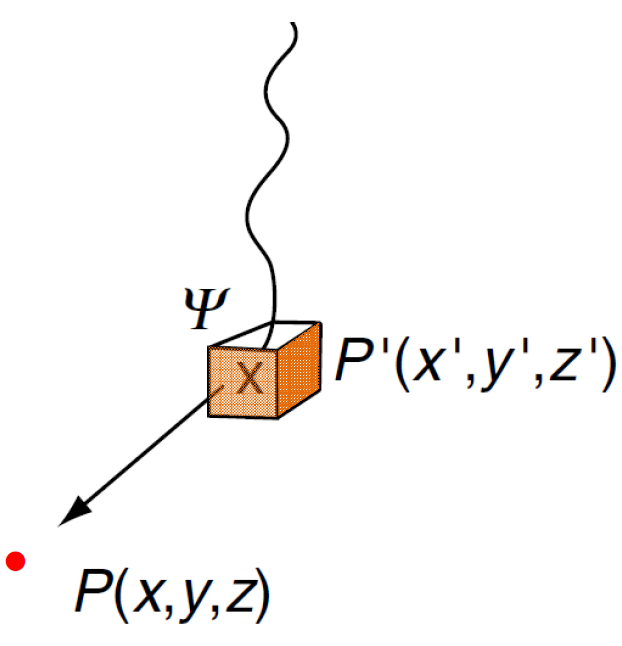
\includegraphics[width=.45\textwidth]{./cap1/superp1.png}
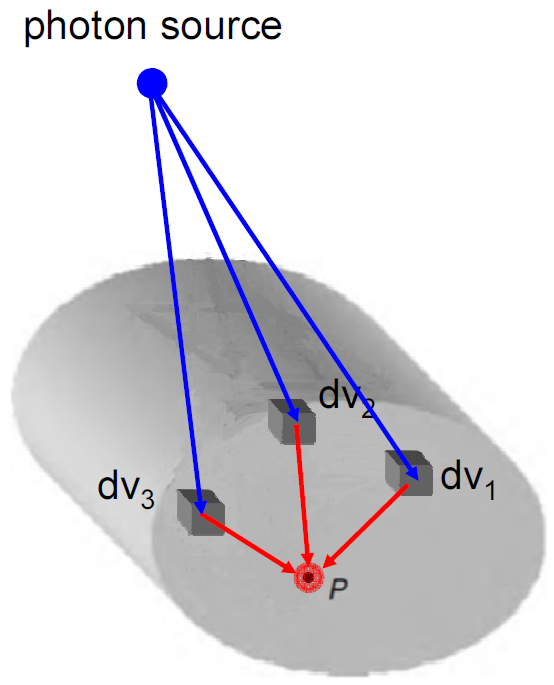
\includegraphics[width=.45\textwidth]{./cap1/superp2.png}
\caption{Il calcolo della dose visto come principio di sovrapposizione.}
\label{fig:superp}
\end{figure}
In particolare, osservando la Fig.\ref{fig:superp}, si nota come la quantità di energia che viene rilasciata in un punto $P$ dipende da infiniti contributi dovuti alle particelle ionizzanti messe in moto dai fotoni nei loro rispettivi centri di interazione $P'\,(\de V_i)$.\\
L'insieme di interazioni dei fotoni primari che avvengono nei punti $P'$ è rappresentato da una quantità denominata TERMA (total-energy-released-in-matter) che conteggia l'energia totale immagazzinata nel volume di interesse. Questa quantità poi verrà trasformata in energia cinetica di particelle secondarie cariche (elettroni) oppure altri fotoni secondari (detti fotoni di scatter).\\
Il TERMA è esprimibile come il prodotto tra la \textit{fluenza di energia primaria} (quantità di energia radiante incidente per unità di superficie [J m$^{-2}$]) e il coefficiente di assorbimento lineare massico del mezzo $(\mu/\rho)$ \cite{Ahnesjo1987}.

Dalla conoscenza del TERMA ($T(x,y,z)$) e della funzione di scatter $s(x'\rightarrow x, y'\rightarrow y, z'\rightarrow z)$ che esprime l'ammontare di energia depositata nel punto $P(x,y,z)$ dovuta all'interazione nel punto $P'(x',y',z')$, la dose assorbita nel punto $P$ è esprimibile con il principio di sovrapposizione:
\begin{align}
D(x,y,z) &=  \int_V \frac{\mu(x',y',z')}{\rho(x',y',z')} \Psi(x',y',z')\,s(x'\rightarrow x, y'\rightarrow y, z'\rightarrow z)\, \de x' \de y' \de z'\\
         &= \int_V T(x',y',z')\,s(x'\rightarrow x, y'\rightarrow y, z'\rightarrow z)\, \de x' \de y' \de z'\\
         &= \int_V T(P')\,s(P'\rightarrow P)\, \de V
\end{align}

Questa equazione è valida nel caso di un fascio di fotoni monoenergetico, tuttavia la generalizzazione è semplice introducendo il TERMA differenziale in energia $T(P',E)$ e la funzione di scatter polienergetica $s(P'\rightarrow P,E)$ ed integrando su tutte le energie coinvolte:
\begin{equation}
\boxed{D(P) = \iint_{E,V} T(P',E)\,s(P'\rightarrow P,E)\, \de V \de E}
\label{eq:superp}
\end{equation}
L'equazione \eqref{eq:superp} rappresenta il principio di sovrapposizione (\textit{superposition}) applicato al calcolo della dose in un volume investito da un fascio di fotoni polienergetico.

Un caso di particolare interesse è quello di un fascio di fotoni monoenergetico e parallelo che investe un mezzo omogeneo. In queste condizioni la funzione di scatter (conosciuta come \textit{energy deposition point kernel} o \textit{point spread kernel} o \textit{kernel di deposizione}) è spazialmente invariante per cui l'integrale di sovrapposizione diventa a tutti gli effetti un integrale di convoluzione facilmente risolvibile grazie alla teoria degli spazi di Fourier.\\
Storicamente il passaggio è stato proprio partire da questo caso più semplice per poi aggiungere le variabili come la divergenza del fascio, la caratteristica polienergetica e le disomogeneità del mezzo che ci riportano al problema più complesso (ma più accurato) della sovrapposizione. Per questo motivo gli algoritmi basati su questa teoria sono conosciuti come algoritmi di \textit{convolution/superposition}.



\section{Il calcolo della dose in RayStation}
Il calcolo della dose nel TPS RayStation fa uso del formalismo illustrato nelle sezioni precedenti e procede in quattro principali passaggi:
\begin{enumerate}
\item Il calcolo della fluenza di energia.
\item Il calcolo del TERMA.
\item L'applicazione delle opportune funzioni di scatter e del principio di sovrapposizione per il calcolo della dose finale.
\item La somma del contributo dovuto alle particelle di contaminazione (elettroni).
\end{enumerate}

\subsection{Il calcolo della fluenza di energia}
\label{sec:fluence}
Questo primo step, consiste in un calcolo geometrico che non tiene conto della presenza del paziente. Si è già notato nella sezione introduttiva (Fig.\ref{fig:processes}) come il fascio in ingresso in un paziente sia costituito da una parte primaria e da una parte che ha interagito con gli elementi della testata (in particolare con il flattening-filter). RayStation tratta queste due componenti con un modello a due sorgenti poste ad una certa distanza lungo la direzione di propagazione del fascio (Fig.\ref{fig:twosources}).
\begin{figure}
\centering
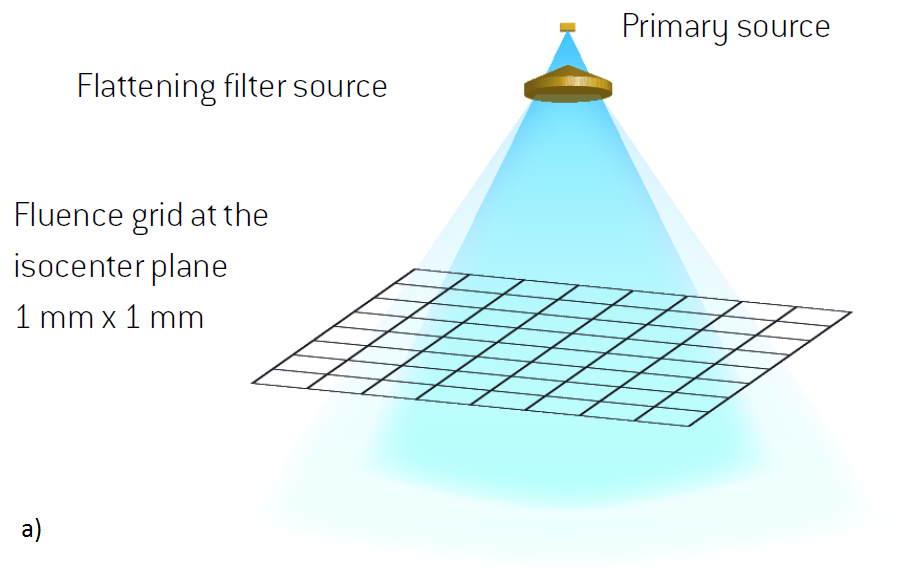
\includegraphics[width=.55\textwidth]{./cap1/twosources.png}
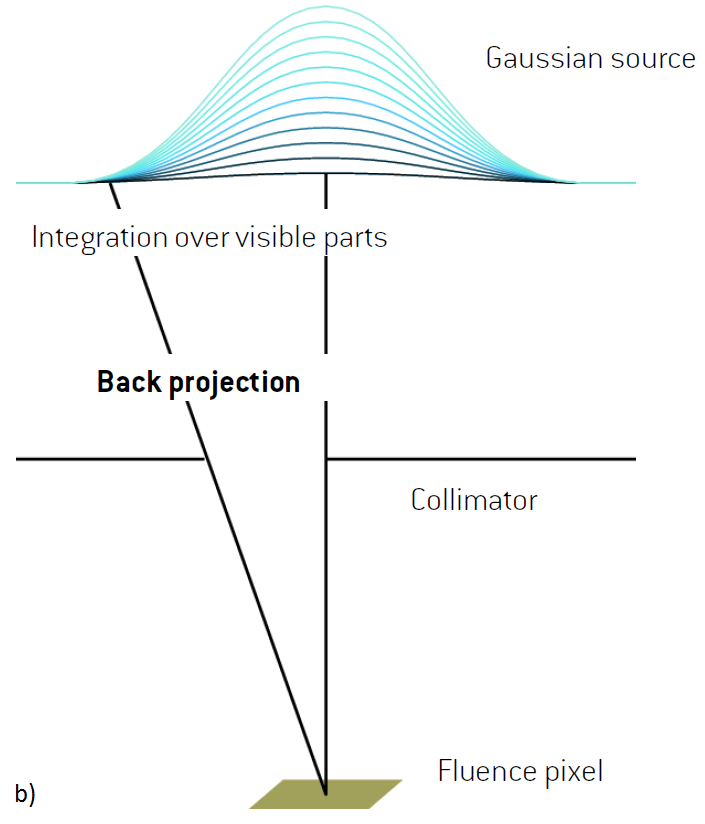
\includegraphics[width=.4\textwidth]{./cap1/source_int.png}
\caption{ (a) Modello a due sorgenti utilizzato per il calcolo della fluenza di energia. (b) Processo di integrazione della parte visibile della sorgente per il calcolo della fluenza.}
\label{fig:twosources}
\end{figure}
La sorgente primaria è modellizzata con un profilo gaussiano ellittico esteso dell'ordine dei mm mentre la sorgente di scatter del flattening-filter è gaussiana circolare estesa dell'ordine dei cm \cite{Chaney1994}.\\
Il calcolo della fluenza viene effettuato su un piano passante per il centro di simmetria rotazionale del LINAC denominato \textit{isocentro} e perpendicolare alla direzione del fascio (Fig.\ref{fig:twosources}a).
Le sorgenti vengono geometricamente proiettate attraverso i collimatori indicati in Fig.\ref{fig:linac} costituiti da blocchi di materiale schermante (\textit{jaws}) e da un dispositivo fatto di lamelle retraibili (\textit{multi-leaf-collimator}) che serve generare conformazioni irregolari del fascio.\\
Matematicamente l'operazione di calcolo della fluenza consiste in un'integrazione pixel per pixel della parte di sorgente \textquotedblleft visibile\textquotedblright{} attraverso i collimatori (Fig.\ref{fig:twosources}b) con un metodo di backprojection.\\
La mappa di fluenza così ottenuta viene corretta per includere alcuni fenomeni come la trasmissione dei collimatori, trasmissione della punta e del bordo delle lamelle (\textit{leaf tip e tongue}\&\textit{groove}), peso relativo delle sorgenti ed altre che verrano discusse in seguito.

In parallelo viene computata la mappa di fluenza per le sorgenti di elettroni di contaminazione. Queste ultime sono gaussiane circolari e poste alla stessa posizione delle sorgenti di fotoni. Esse sono divise in primaria e di scatter del flattening filter la cui intensità è espressa in percentuale rispetto alla fluenza dei fotoni.

\subsection{Il calcolo del TERMA}
Il TERMA costituisce la prima parte dell'integrale per il calcolo della dose assorbita. Esso rappresenta in pratica l'assorbimento della fluenza di energia che attraversa il paziente. A partire da questo assorbimento verranno poi applicate le funzioni di scatter per generare la distribuzione di dose.\\
Il TERMA differenziale in energia è stato definito nella Sez.\ref{sec:teoria_conv} in accordo con \cite{Ahnesjo1999}:
\begin{equation}
\label{eq:termaE}
T(\vec{r'},E) = \frac{\mu}{\rho}(\vec{r'},E)\,\Psi(\vec{r'},E)
\end{equation}
dove $\vec{r'}$ è la coordinata del punto di interazione primaria.

Il paziente è modellizzato all'interno del TPS tramite uno studio di tomografia computerizzata che contiene una mappa di densità dei tessuti. Questo permette di conoscere il primo termine dell'Eq.\eqref{eq:termaE} \cite{RaySearchLaboratories2014}.\\
Il secondo termine è la fluenza di energia calcolata nello step precedente. Per il calcolo del TERMA, detta fluenza viene proiettata verso la sorgente primaria fino a coincidere con la superficie del paziente ($\Psi(\vec{r_0},E)$) e poi viene riproiettata verso il basso tenendo conto dell'assorbimento nei tessuti (esponenziale con il coefficiente di assorbimento) e della divergenza del fascio (decadimento col quadrato della distanza):
\begin{equation}
\label{eq:fluence}
\Psi(\vec{r'},E) = \frac{|\vec{r_0}|^2}{|\vec{r'}|^2}\Psi(\vec{r_0},E)\,\exp{\left( -\int_{\vec{r_0}}^{\vec{r'}} \mu(\vec{r'},E) \de l \right)}
\end{equation}
L'integrale del coefficiente di assorbimento nella precedente equazione viene discretizzato nel TPS su una griglia di voxel cubici detta \textit{dose grid}. Questi voxel campionano le densità fornite dalla CT da cui viene ricavato il coefficiente di assorbimento locale (vedi Fig.\ref{fig:terma}). A questo punto, moltiplicando entrambi i termini dell'equazione \eqref{eq:termaE} si ottiene la distribuzione di TERMA.

\begin{figure}
\centering
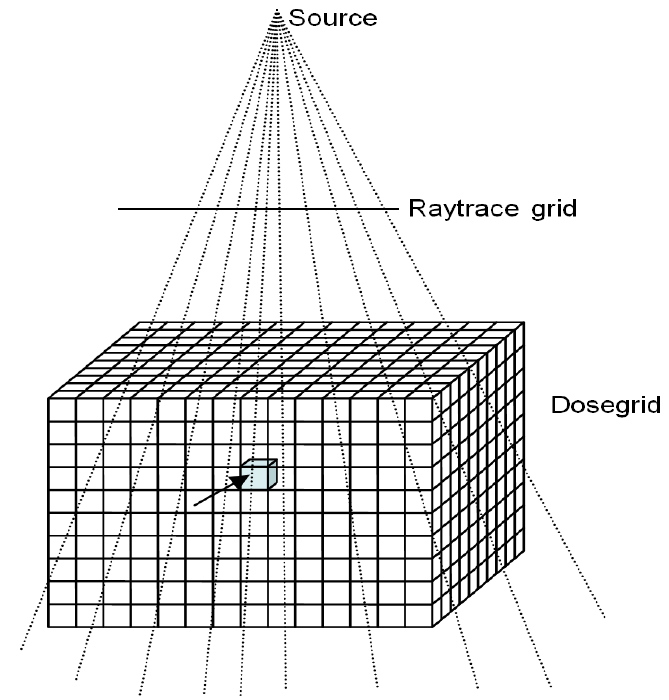
\includegraphics[width=.4\textwidth]{./cap1/terma_1.png}
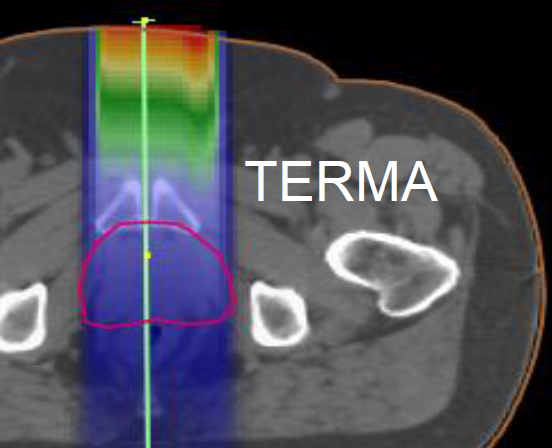
\includegraphics[width=.5\textwidth]{./cap1/terma_2.png}
\caption{Sinistra: griglia per il calcolo del TERMA e della dose. Da notare che per motivi di velocità la divergenza del fascio viene approssimata come proveniente unicamente dalla sorgente primaria e non dal flattening filter. Destra: distribuzione del TERMA computato su una scansione CT di un paziente.}
\label{fig:terma}
\end{figure}

\subsection{Applicazione delle funzioni di scatter}
Se l'energia totale rilasciata dai fotoni in un voxel fosse interamente assorbita in esso, la distribuzione di TERMA coinciderebbe con la dose assorbita.\\
\begin{figure}
\centering
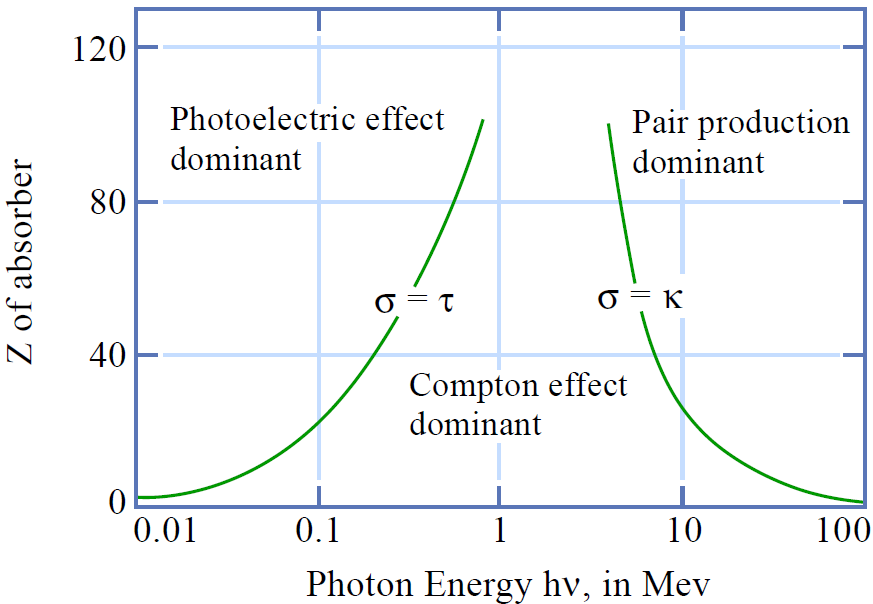
\includegraphics[width=.7\textwidth]{./cap1/compt_dom.png}
\caption{Prevalenza degli effetti di interazione dei fotoni con la materia. L'effetto Compton è prevalente per le energie e i materiali tipici della radioterapia.}
\label{fig:compt_dom}
\end{figure}
Tuttavia alle energie tipiche dei fotoni utilizzati in radioterapia l'effetto predominante è l'effetto Compton (Fig.\ref{fig:compt_dom}).

Una modellizzazione completa del trasporto del fotone diffuso e dell'elettrone messo in moto richiede un approccio statistico di tipo Monte Carlo computazionalmente molto dispendioso che tuttavia negli ultimi anni sta diventando disponibile commercialmente grazie all'incremento della potenza di calcolo dei computer.\\
L'approccio convolution/superposition racchiude i processi statistici di deposizione dell'energia nella funzione di scatter introdotta nell'Eq.\eqref{eq:superp}.\\
Questa funzione è ottenibile a partire da una simulazione Monte Carlo in cui un unico fotone viene fatto interagire forzatamente all'interno di un volume omogeneo di acqua e si va ad osservare la deposizione della dose che ne deriva.\\
Questa operazione è stata effettuata da Mackie \cite{Mackie1985} utilizzando il software Monte Carlo EGS sviluppato dallo Stanford Linear Accelerator Center che pubblicò nella metà degli anni '80 delle funzioni di scatter discretizzate in forma tabulare proponendo un metodo di convoluzione del tipo look-up-table (prontamente implementabile in un computer). Propose anche un metodo per riscalare le funzioni di scatter con la densità per poter calcolare la dose in mezzi diversi dall'acqua senza dover rieffettuare la simulazione Monte Carlo (vedi Fig.\ref{fig:mackie_kernels}).
\begin{figure}
\centering
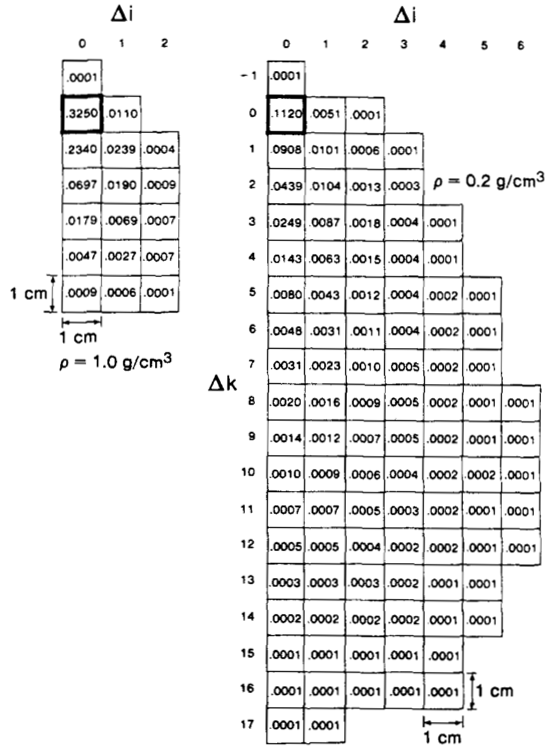
\includegraphics[width=.8\textwidth]{./cap1/mackie_kernels.png}
\caption{Funzione di scatter calcolate da Mackie \cite{Mackie1985} per un fotone da 15MV. Da notare come l'assunzione di deposizione locale dell'energia non è accettabile (nel punto di interazione cade il 32.5\% della dose totale per l'acqua e l'11.2\% per un mezzo di densità 0.2g/cc.)}
\label{fig:mackie_kernels}
\end{figure}

Applicando le funzioni di scatter (kernel) ai punti di deposizione del TERMA, è possibile arrivare alla dose assorbita in maniera triviale utilizzando il metodo di sovrapposizione. Questa operazione su una griglia di $N^3$ voxel risulta essere un problema  di ordine $N^6$ \cite{Ahnesjo1999}. Se si aggiunge l'operazione di scaling dei kernel per la densità il problema diventa di ordine $N^7$ difficilmente gestibile anche con le moderne potenze di calcolo\footnote{Se immaginiamo di discretizzare un paziente di dimensioni $20x20x20$ cm$^3$ con voxel di lato $0.3$ cm otteniamo una griglia di circa $70x70x70$ voxel. Il numero di operazioni da effettuare con un metodo di sovrapposizione triviale sarebbe $70^7\approx 10^{13}$. Disponendo di un computer capace di effettuare operazioni con frequenza dell'ordine del GHz$\equiv 10^9$ il tempo di risolvere $10^{13}$ operazioni sarebbe $t=10^{13}/10^9=10^5\,sec\approx 2\, ore!$.}. Per questo motivo, gran parte della ricerca successiva allo sviluppo del metodo di convolution/superposition fu orientata a sviluppare delle approssimazioni che permettessero il calcolo della dose in tempi compatibili con una routine di tipo clinico.

\subsection{L'approssimazione \textit{collapsed-cone}}
Lo stesso Mackie assieme a Reckwerdt \cite{Reckwerdt1992} propose un'approssimazione che consisteva nel calcolare l'integrale di sovrapposizione solo lungo determinate direzioni. Indipendentemente, Ahnesj\"{o} nel 1989 seguendo lo stesso approccio, pubblica un articolo \cite{Ahnesjo1989} che propone un metodo di soluzione del problema convolution/superposition denominato \textit{collapsed-cone} e lo confronta con la tecnica Monte Carlo ottenendo risultati eccellenti per l'epoca. Questi risultati rappresentano ancora oggi il benchmark per il calcolo della dose con metodi non statistici.

\begin{figure}[!t]
\centering
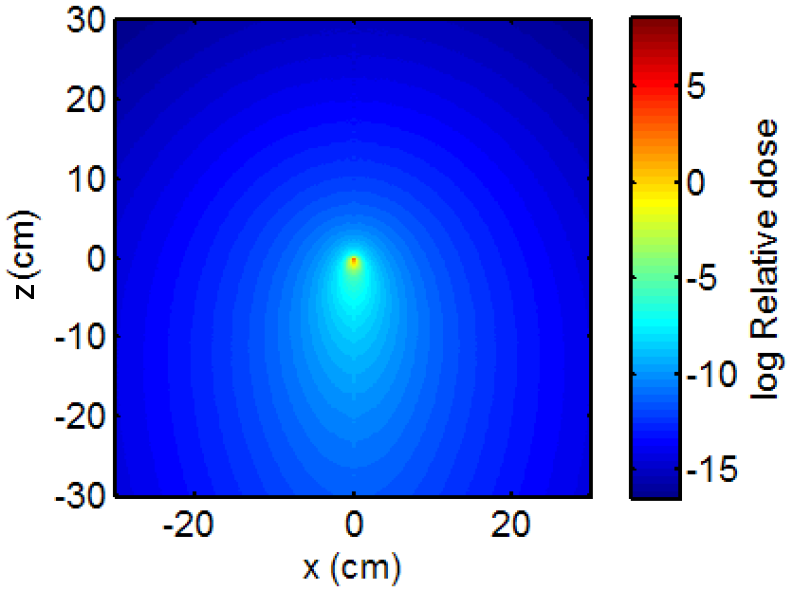
\includegraphics[width=.45\textwidth]{./cap1/kern_ray1.png}$\quad$
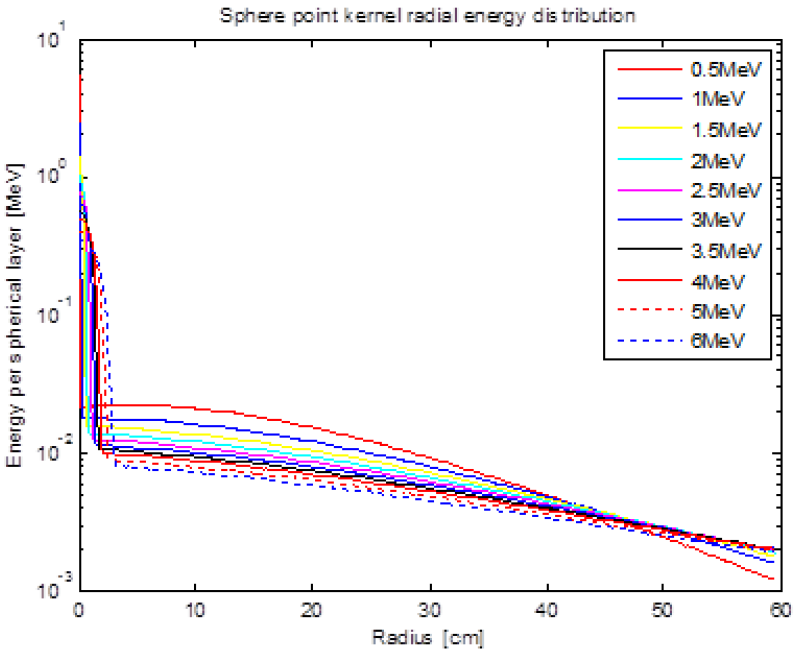
\includegraphics[width=.45\textwidth]{./cap1/kern_ray2.png}
\caption{Sinistra: distribuzione planare di un kernel di deposizione. Destra: distribuzione 1D di alcuni kernel al variare dell'energia; da notare una prima parte di rilascio rapido di energia dovuta agli elettroni Compton ed una parte più estesa dovuta ai fotoni secondari diffusi che a loro volta re-interagiscono con il mezzo.}
\label{fig:kern_ray}
\end{figure}
In Fig.\ref{fig:kern_ray} è possibile osservare la distribuzione spaziale tipica di alcuni kernel di deposizione.

\vspace{.2cm}
L'approssimazione di collapsed cone consiste in pratica in una discretizzazione del kernel che è necessaria per poter risolvere l'equazione di sovrapposizione \eqref{eq:superp} per via computazionale. Ahnesj\"{o} notò che un metodo triviale di discretizzazione ad esempio con dei semplici raggi, può portare ad un errore di sampling ampio a causa della rapidità di rilascio di energia nei primi cm di interazione \cite{Ahnesjo1989} (Fig.\ref{fig:kern_ray}) (i.e. una larga parte di deposizione di energia non viene conteggiata a meno di usare un campionamento angolare fittissimo).\\
Per questo Ahnesj\"{o} propose di discretizzare i kernel in coordinate sferiche con dei coni aventi il vertice nel punto di interazione e sottendenti un certo angolo solido. Tutte le deposizioni di energia contenute all'interno della superficie conica che sottende l'angolo solido vengono \textquotedblleft\textit{collassate}\textquotedblright{} sull'asse del cono stesso. In questo modo l'energia totale depositata risulta soltanto spazialmente ridistribuita ma viene conteggiata per intero.

Matematicamente l'approssimazione di collapsed cone consiste dapprima in un fit analitico del kernel di deposizione che in coordinate sferiche ha la seguente forma:
\begin{equation}
\label{eq:kern_fit}
s(r,\theta) = \frac{A_\theta e^{-a_\theta r} + B_\theta e^{-b_\theta r}}{r^2}
\end{equation}
dove $A_\theta,\,a_\theta,\,B_\theta$ e $b_\theta$ sono parametri di fit che dipendono dall'angolo di scatter $\theta$. I due termini esponenziali descrivono l'uno la caduta rapida del kernel dovuto agli elettroni Compton primari e l'altro la coda più lenta dovuta alle interazioni di scatter secondarie (Fig.\ref{fig:kern_ray}). Da notare che il kernel possiede una simmetria cilindrica per cui l'angolo $\phi$ non è esplicitato. La validità di questo fit è mostrata in Fig.\ref{fig:kern_fit}.
\begin{figure}
\centering
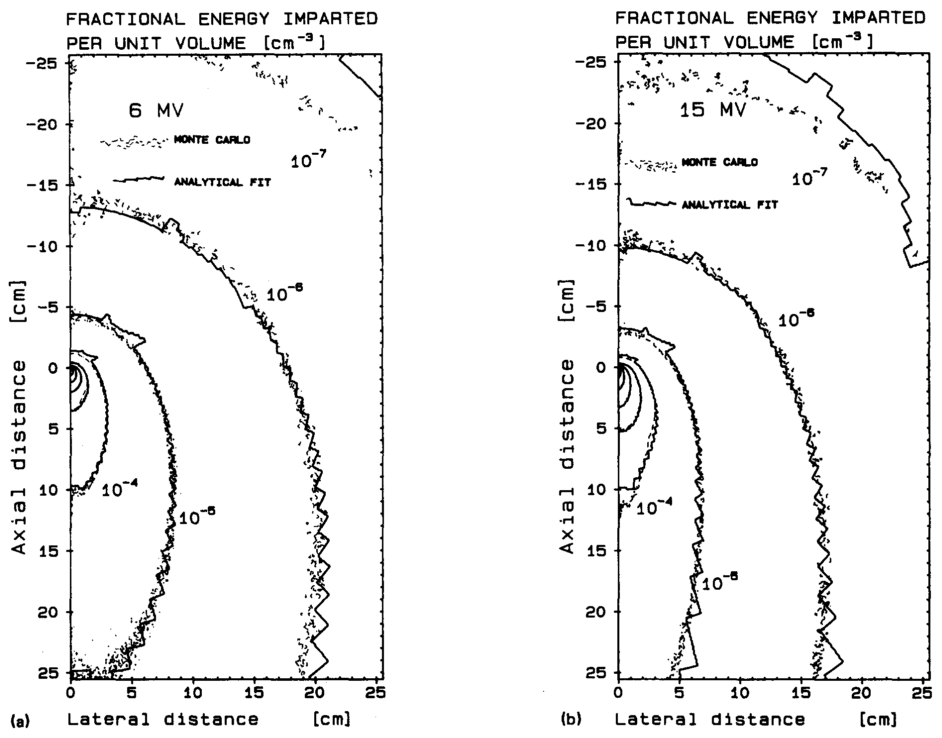
\includegraphics[width=.8\textwidth]{./cap1/kern_fit.png}
\caption{Fit analitico dei kernel di deposizione per un fotone da 6MV (a) e da 15MV (b). Tratto da \cite{Ahnesjo1989}.}
\label{fig:kern_fit}
\end{figure}

Stabilendo un angolo solido $\Omega_i$, l'operazione di \virg{collapsing} è un'integrazione in coordinate sferiche del kernel espresso dalla \eqref{eq:kern_fit} (vedi anche Fig.\ref{fig:kern_collaps}):
\begin{equation}
\iint_{\Omega_i} s(r,\theta) r^2\de \Omega_i = A_{\Omega_i} e^{-a_{\Omega_i} r} + B_{\Omega_i} e^{-b_{\Omega_i} r} \equiv K(r,\Omega_i)
\end{equation}
La funzione $K(r,\Omega_i)$ è quella da convolvere con la mappa del TERMA per arrivare alla mappa di dose assorbita.

Il metodo collapsed-cone è stato dimostrato \cite{Ahnesjo1999} comportare un numero di operazioni dell'ordine di $MN^3$ dove $M$ è il numero di settori in cui viene diviso l'angolo solido ed $N$ è il numero di voxel della griglia di dose/TERMA. Questo è da confrontare con l'ordine $N^7$ in caso di applicazione triviale del metodo di sovrapposizione.

\begin{figure}
\centering
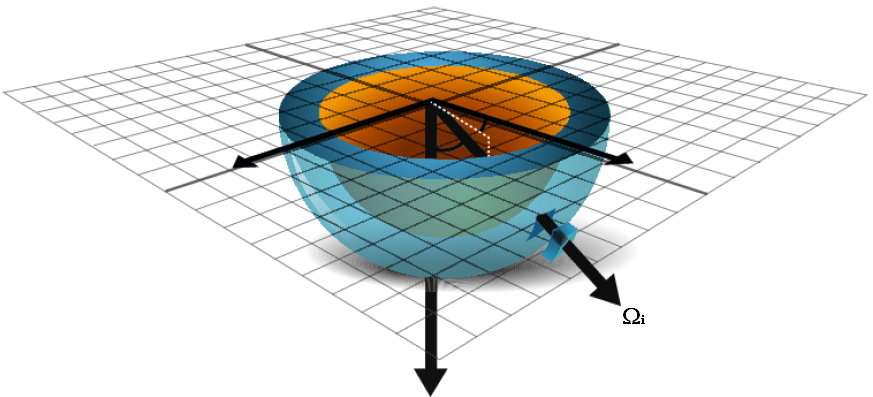
\includegraphics[width=\textwidth]{./cap1/kern_collaps.png}
\caption{Operazione di \textit{collapsing} dei kernel all'interno di segmenti conici definiti dall'angolo solido $\Omega_i$.}
\label{fig:kern_collaps}
\end{figure}

In RayStation il numero di settori in cui viene discretizzato il kernel è 128 che corrispondono a 8 direzioni lungo l'angolo di scatter $\theta$ e 16 lungo l'angolo di simmetria cilindrica $\phi$. Il campionamento è più fitto nella direzione di propagazione del fascio dove è presente il gradiente più intenso.

\subsection{La generalizzazione al caso polienergetico}
Un tipico fascio di fotoni generato da un LINAC per radioterapia contiene uno spettro polienergetico. Inoltre lo spettro subisce uno spostamento verso energie più alte a causa dell'attraversamento della materia (effetto di \textit{depth-hardening}). Questo suggerisce il fatto che non è possibile considerare un unico kernel di deposizione nel passaggio dal TERMA alla dose. Boyer et al. assieme a Zhu e Van Dyk \cite{Boyer1989,Zhu1995} hanno dimostrato come una discretizzazione in 5 bin sia sufficiente a rappresentare lo spettro di un LINAC da 6MV. Sulla base di ciò Papanikolaou et al. \cite{Papanikolaou1993} hanno investigato i possibili metodi di estensione del metodo convolution al caso polienergetico dimostrando che è sufficiente combinare kernel monoergetici pesati con le relative componenti spettrali. Inoltre dimostrano come il problema del depth-hardening può essere risolto riscalando i kernel con dei fattori che dipendono dalla lunghezza radiologica attraversata.

Per applicare questi principi, nel TPS sono memorizzati una serie di point spread kernel computati con il motore Monte Carlo EDKnrc incluso in EGS4nrc per le seguenti energie del fotone primario incidente: 0.5, 1, 1.5, 2, 2.5, 3, 3.5, 4, 5, 6, 7, 8, 9 10, 12, 14, 16, 18, 20 MeV. Queste energie corrispondono ai bin implementati in RayStation per rappresentare uno spettro fotonico (es. per un fascio da 6 MV i bin coinvolti vanno da 0.5 a 6 MV).\\
Il peso di ogni componente spettrale viene stabilito in fase di modellizzazione (vedi cap. successivi). Per ora ci interessa sapere che, fissato lo spettro, viene costruito il kernel polienergetico secondo le indicazioni di Papanikolaou et al. \cite{Papanikolaou1993} (media pesata con le componenti spettrali). In seguito viene costruita una libreria di 600 kernel in un intervallo di lunghezze radiologiche da -100 g/cm$^2$ a 200 g/cm$^2$\footnote{Nota: lunghezze radiologiche negative sono necessarie per tenere in conto l'effetto di \textit{off-axis softening} dovuto alla presenza del flattening-filter di cui si parlerà nei capitoli successivi.} da essere utilizzate per tenere conto dell'effetto di \textit{depth-hardening}.


\subsection{La generalizzazione al caso disomogeneo}
Un ulteriore fenomeno da tenere in conto nell'applicazione dei point spread kernel è la disomogeneità del mezzo. In condizioni standard i kernel sono calcolati in un volume omogeneo di acqua, tuttavia la deposizione di energia cambia se i processi di ionizzazione avvengono in un mezzo differente dall'acqua.\\
Woo e Cunningham \cite{Woo1990} assieme a Mackie \cite{Mackie1985} hanno dimostrato come sia possibile evitare di ricalcolare i kernel per ogni situazione considerando tutte le lunghezze fisiche ($l$) come lunghezze radiologiche ($\rho\,l$) (dove $\rho$ è la densità del mezzo). La base di questa metodologia era in realtà nota già prima dell'avvento degli algoritmi di convolution come Teorema di O'Connor \cite{OConnor1957}.\\
\begin{figure}[!t]
\centering
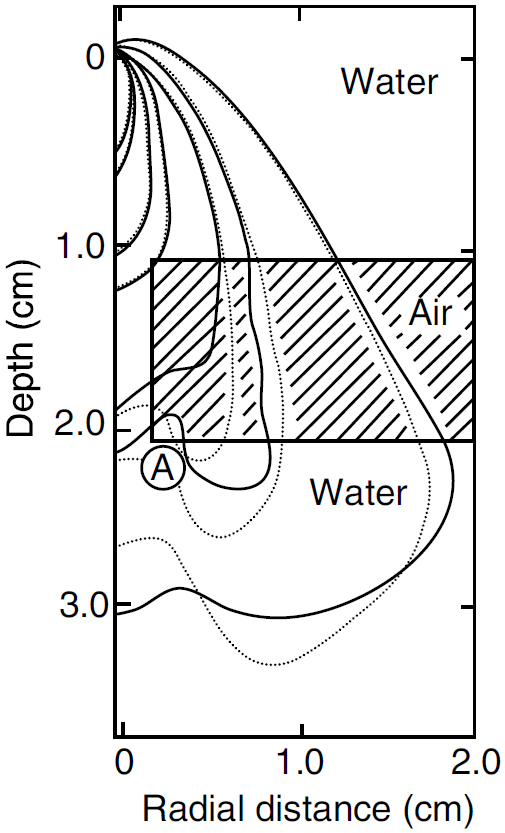
\includegraphics[width=.4\textwidth]{./cap1/kern_dens.png}
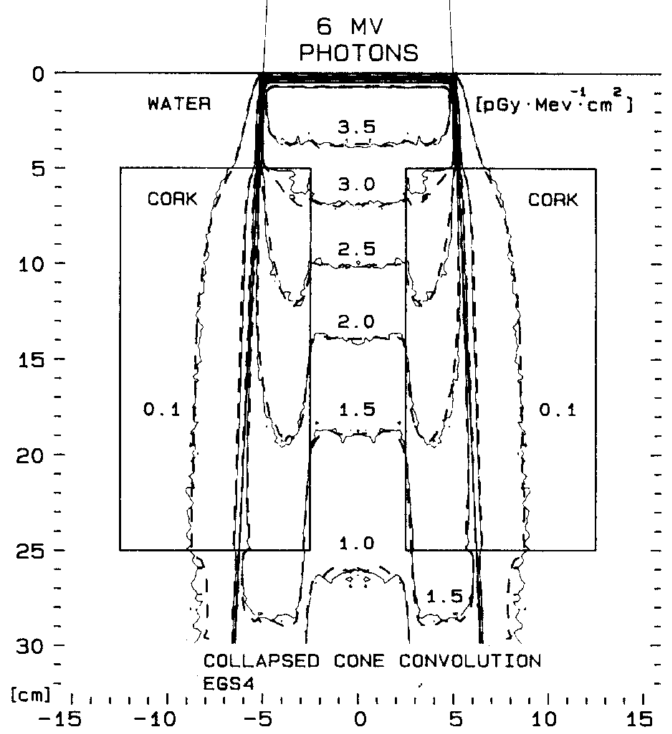
\includegraphics[width=.59\textwidth]{./cap1/kern_dens2.png}
\caption{Sinistra: Contronto tra un kernel calcolato direttamente con un metodo Monte Carlo (linea solida) e un kernel calcolato in condizioni omogenee riscalato secondo la lunghezza radiologica (linea tratteggiata); le isolinee corrispondono ad una dose relativa di 1000, 500, 100, 50, 10, 5, 1; il punto A posizionato appena sotto l'interfaccia aria/acqua presenta la massima discrepanza (50\%). Destra: effetto globale su un insieme di interazioni; un \textit{averaging} delle incertezze sui singoli kernel si risolve in un accordo accettabile su un fantoccio complesso che simula un torace \cite{Woo1990,Arnfield2000,Ahnesjo1989}.}
\label{fig:kern_dens}
\end{figure}
Nella Fig.\ref{fig:kern_dens} si può notare l'errore che si commette adottando il metodo suggerito in una configurazione di disomogeneità aria/acqua che può simulare una situazione tessuto/polmone. Nonostante l'accordo non sia perfetto, Woo e Cunnigham \cite{Woo1990} assieme ad Arnfield et al. \cite{Arnfield2000} e lo stesso Ahnesj\"{o} \cite{Ahnesjo1989} hanno dimostrato che su un insieme di interazioni interviene un effetto di \textit{averaging} di tutti i kernel vicini per cui discrepanze significative rimangono solo in condizioni si estrema disomogeneità, ossia vicino a delle interfacce in cui la densità cambia repentinamente (vedi Fig.\ref{fig:kern_dens}).

Aggiungendo  la generalizzazione al caso disomogeneo l'equazione di sovrapposizione \eqref{eq:superp} per il calcolo della dose può essere riscritta \cite{Khan2010}:
\begin{equation}
D(\vec{r}) = \iint_{E,V} T_E(\rho_{\vec{r'}} \cdot \vec{r})\, s_E(\rho_{\vec{r}-\vec{r'}}\cdot (\vec{r}-\vec{r'}))\de\vec{r'} \de E
\end{equation}
dove $(\rho_{\vec{r'}} \cdot \vec{r})$ è la lunghezza radiologica dalla sorgente fino al punto di interazione primaria (ove viene rilasciato il TERMA) e $\rho_{\vec{r}-\vec{r'}}\cdot (\vec{r}-\vec{r'})$ è la lunghezza radiologica dal punto di interazione primaria al punto di deposizione della dose.

\begin{figure}
\centering
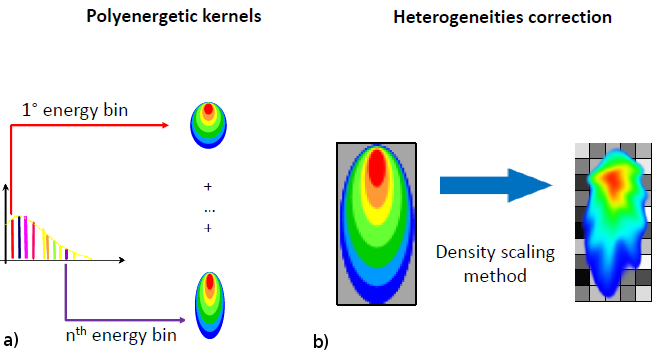
\includegraphics[width=\textwidth]{./cap1/kern_trans.png}
\caption{Sinistra: figura schematica del metodo con cui si costruisce il kernel polienergetico (combinazione di kernel monoenergetici pesati con la componente spettrale). Destra: figura schematica che rappresenta come il kernel si modifica quando viene riscalato tenendo conto delle lunghezze radiologiche attraversate nelle varie direzioni.}
\label{fig:kern_trans}
\end{figure}

In Fig.\ref{fig:kern_trans} sono riportati due diagrammi schematici riguardo le generalizzazioni al caso polienergetico e disomogeneo.


In Fig.\ref{fig:terma_dose} è riportato graficamente il processo di passaggio dal TERMA alla dose. Quello che si può notare è che l'applicazione dei kernel di deposizione comporta un \textquotedblleft\textit{blurring}\textquotedblright{} e un prolungamento della distribuzione di TERMA che è dovuto proprio al movimento delle particelle ionizzanti secondarie messe in moto dai fotoni primari e diffusi.
\begin{figure}
\centering
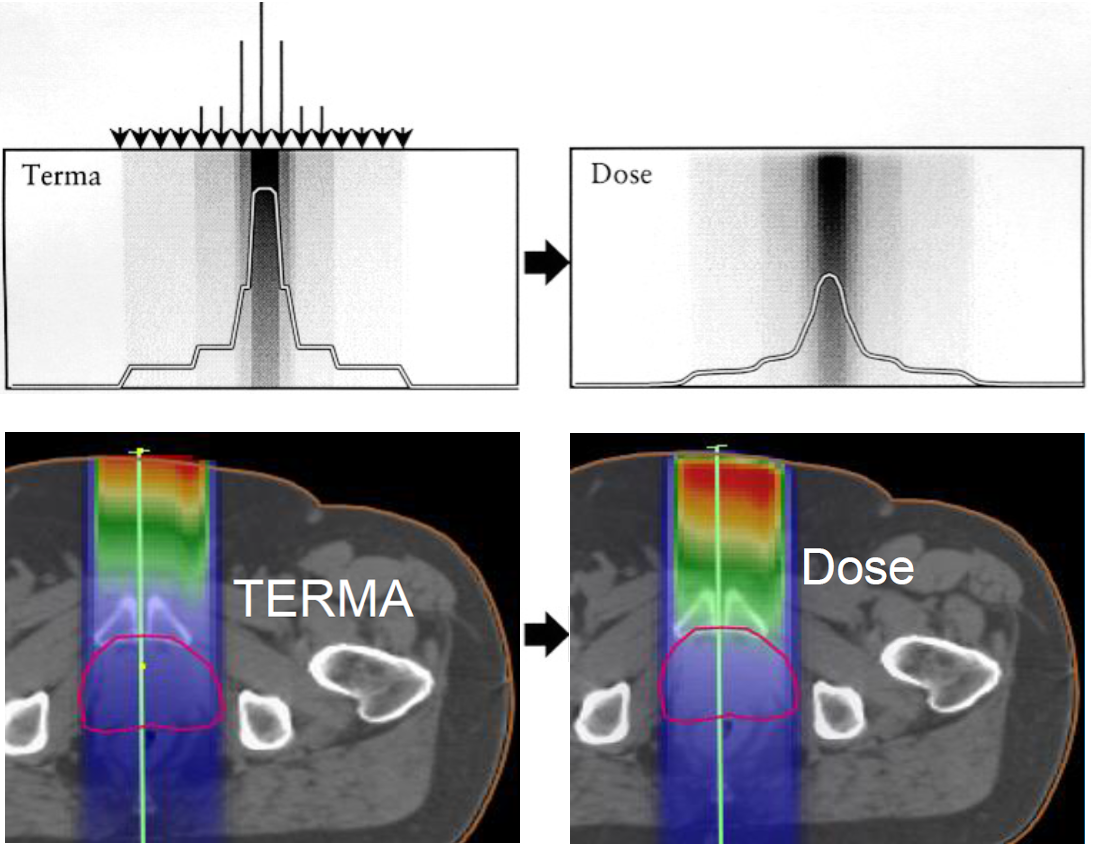
\includegraphics[width=.8\textwidth]{./cap1/terma_dose.png}
\caption{In alto: trasformazione del TERMA in dose in condizioni di omogeneità. In basso: trasformazione del TERMA in dose su una scansione CT di un paziente reale. Da notare è l'effetto di \textquotedblleft\textit{blurring}\textquotedblright{} dovuto all'applicazione dei kernel di deposizione.}
\label{fig:terma_dose}
\end{figure}



\section{Approssimazioni aggiuntive}
Nella sezione precedente sono state mostrate le approssimazioni intrinseche dell'algoritmo \textit{collapsed-cone}. In questa sezione evidenziamo delle ulteriori approssimazioni adottate in RayStation orientate all'aumento di velocità del calcolo della dose.

\subsection{L'approssimazione \textit{no-kernel-tilting}}
Un fascio di fotoni generato da un LINAC è tipicamente divergente all'aumentare della distanza dalla sorgente. I kernel di deposizione dell'energia sono calcolati per un fascio che incide verticalmente ed hanno l'asse orientato nella medesima direzione. Un'applicazione rigorosa del metodo convolution/superposition richiederebbe la rotazione dei kernel per allinearli lungo l'angolo di incidenza del raggio primario (vedi Fig.\ref{fig:kern_tilt}).\\
\begin{figure}
\centering
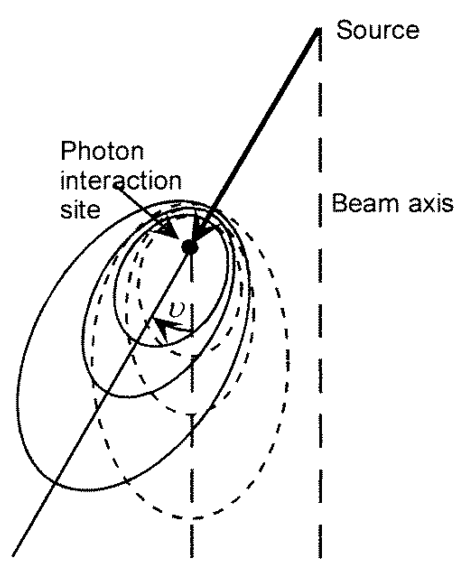
\includegraphics[width=.35\textwidth]{./cap1/kern_tilt.png}
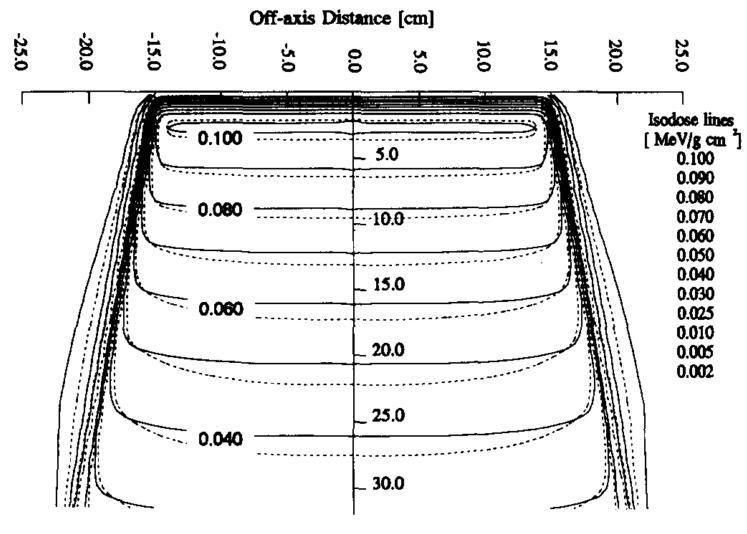
\includegraphics[width=.6\textwidth]{./cap1/kern_tilt_b.png}
\caption{Sinistra: I kernel di deposizione dovrebbero essere ruotati dello stesso angolo di incidenza $\nu$ del raggio primario; tuttavia per ridurre considerevolmente i tempi di calcolo, si applicano kernel con orientazione verticale. Destra: il non ruotare i kernel comporta una deposizione di dose maggiore verso il centro del fascio (linea tratteggiata) confrontata con la dose calcolata senza approssimazione (linea solida); questo può essere corretto secondo \cite{Papanikolaou1993} (vedi testo).} 
\label{fig:kern_tilt}
\end{figure}
Questa operazione implicherebbe molteplici operazioni di rotazione di matrici \cite{Sharpe1997} con il risultato di aumentare considerevolmente il tempo di calcolo della dose. 
%Oltre a questo, un ulteriore grande vantaggio dell'approssimazione \textit{no-kernel-tilting} consiste nel fatto di poter calcolare solo una volta le intersezioni dei raggi uscenti dai kernel con la griglia di dose\footnote{Operazione nota come \textit{raytracing}.} e di riutilizzare i risultati per i voxel successivi.
Per questo motivo vari autori hanno sviluppato dei metodi che consentissero di applicare kernel di deposizione non ruotati (\textit{no-kernel-tilting}) \cite{Sharpe1997,Papanikolaou1993}.

In RayStation è implementato il metodo suggerito da Papanikolaou et al. \cite{Papanikolaou1993}. L'idea di questo metodo sta nel considerare che, non ruotando i kernel, si ha un accumulo di dose maggiore verso il centro del fascio (Fig.\ref{fig:kern_tilt}).\\ 
Papanikolaou ha dimostrato come questo può essere recuperato con i seguenti passaggi:
\begin{enumerate}
\item Si rimuove la divergenza dalla fluenza di energia (termine $|\vec{r_0}|^2/|\vec{r'}|^2$ nell'Eq.\eqref{eq:fluence}).
\item Si applicano i point spread kernel con l'approssimazione di \textit{no-tilting}.
\item Si riapplica la divergenza riscalando la dose calcolata con il fattore $|\vec{r_0}|^2/|\vec{r}|^2$ dove $\vec{r}$ è la coordinata di calcolo della dose (diversa dalla coordinata di rilascio del TERMA $\vec{r'}$).
\end{enumerate}
L'effetto dell'operazione n.1 è quello di aumentare la fluenza di energia lontano dal centro del fascio. Applicando poi i punti 2 e 3 si arriva ad una distribuzione in cui la dose approssima quella calcolata considerando i kernel ruotati.\\
Sharpe e Papanikolaou \cite{Sharpe1997,Papanikolaou1993} hanno evidenziato come l'approssimazione di \textit{no-tilting} dei kernel presenti i suoi limiti solo in situazioni difficilmente realizzabili clinicamente. In particolare, discrepanze oltre il 3\% si osservano in caso di basse distanze sorgente-superficie del paziente (SSD $< 70$ cm) e campi estesi ($> 20x20$ cm$^2$).



\subsection{Approssimazioni \textit{full-TERMA-deposition} e \textit{adaptive interpolation}}
Queste due approssimazioni sono volte ad evitare di applicare rigorosamente il metodo di collapsed-cone-superposition su ogni voxel della griglia di dose.\\
A questo proposito, una prima approssimazione consiste nella \textit{full-TERMA-deposition} che può essere riassunta in quattro principali step:
\begin{enumerate}
\item Alla fine del calcolo della distribuzione di TERMA vengono identificati quei voxel in cui è stato depositato un TERMA minore dello 0.5\% del massimo TERMA rilasciato nel volume.
\item A partire da questi voxel viene costruita una iso-superficie che viene poi espansa di una lunghezza radiologica di 5 cm isotropicamente.
\item Al di fuori della superficie precedentemente calcolata non viene effettuato il trasporto del TERMA con l'algoritmo collapsed-cone bensì si assume un rilascio locale di tutta l'energia.
\item All'interno del volume compreso tra la superficie TERMA$_i= 0.5\%$ TERMA$_{max}$ e la sua espansione di $5$ cm  il trasporto avviene solo su alcune delle 128 direzioni del kernel di deposizione. 
\end{enumerate}
Questa approssimazione è stata osservata generare un'errore sul calcolo della dose minore dello 0.2\% su punti peraltro a bassa rilevanza clinica \cite{RaySearchLaboratories2014}.\\

\begin{figure}
\centering
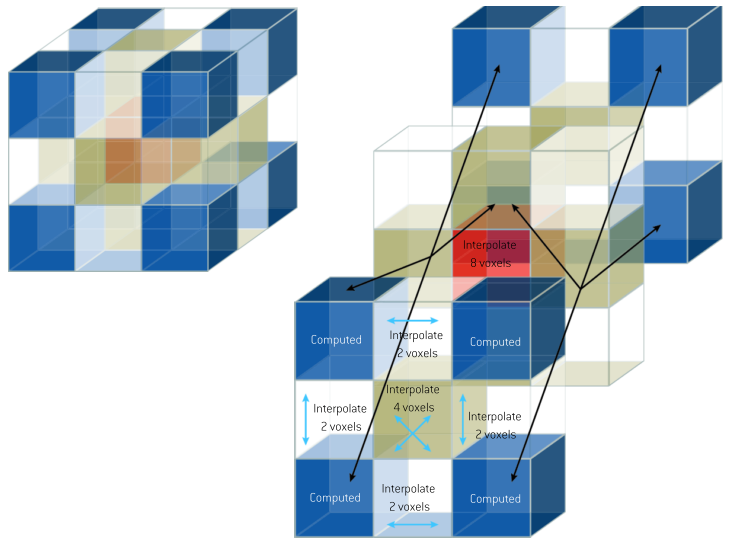
\includegraphics[width=\textwidth]{./cap1/dose_interp.png}
\caption{L'approssimazione di \textit{adaptive interpolation}. I voxel in blu sono quelli calcolati con l'algoritmo collapsed-cone.}
\label{fig:dose_interp}
\end{figure}

La seconda approssimazione di \textit{adaptive interpolation} si basa su un preliminare calcolo della dose a bassa risoluzione per identificare zone a basso od alto gradiente. Per le zone a basso gradiente la dose nei voxel rimanenti viene calcolata con la media dei voxel adiacenti; per le zone ad alto gradiente viene applicato l'algoritmo completo. In particolare gli step che vengono seguiti sono riassumibili nei seguenti punti:
\begin{enumerate}
\item Dopo il calcolo della distribuzione di TERMA si effettua un primo calcolo della dose ogni due voxel come illustrato nella Fig.\ref{fig:dose_interp}.
\item Un voxel viene considerato appartenere ad una zona a basso gradiente se la massima differenza tra il TERMA nei voxel adiacenti è minore dello 0.2\% e la massima differenza in dose è minore del 5\% della dose massima.
\item Per i voxel appartenenti alla zona a basso gradiente la dose viene calcolata mediando i voxel adiacenti che possono essere in numero di 2, 4 o 8 a seconda della posizione (vedi Fig.\ref{fig:dose_interp}).
\item Per i voxel appartenenti alla zona ad alto gradiente viene applicato l'algoritmo completo.
\end{enumerate}
Per un semplice campo $10x10$ cm$^2$ ed energia 6 MV, la distribuzione di dose calcolata senza applicare la \textit{adaptive interpolation} si correla con la dose calcolata utilizzando l'approssimazione con un coefficiente di correlazione maggiore di 0.99999. Gli errori più rilevanti si registrano vicino alla penombra del fascio dove rimangono comunque entro il 2\% \cite{RaySearchLaboratories2014}.


\section{Dose aggiuntiva da elettroni di contaminazione}
Come già accennato nella sezione introduttiva (Fig.\ref{fig:processes}), nei primi centimetri di tessuto una parte rilevante della dose totale è dovuta agli elettroni di contaminazione del fascio fotonico. Questi elettroni si originano prevalentemente da processi di scatter dei fotoni con i collimatori e il flattening-filter all'interno della testata.\\
Alle energie tipiche della radioterapia, la deposizione della dose di un fascio elettronico avviene repentinamente all'aumentare della profondità con un limitato peso dovuto a fenomeni di ionizzazione secondaria (vedi Fig.\ref{fig:electr_enloss}).
\begin{figure}
\centering
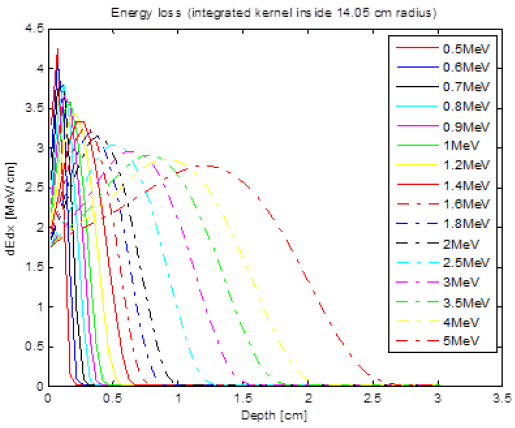
\includegraphics[width=.5\textwidth]{./cap1/electr_enloss.png}
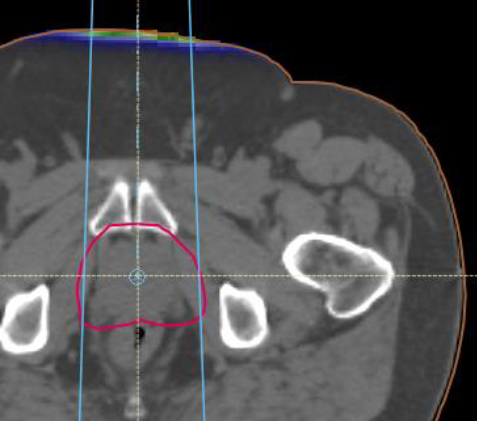
\includegraphics[width=.45\textwidth]{./cap1/electr_doseCT.png}
\caption{Sinistra: diagrammi della dose rilasciata in funzione della profondità di un fascio di elettroni a varie energie. Destra: distribuzione di dose dovuta ad elettroni di contaminazione del fascio calcolata su una CT. Da notare è che questa dose è importante solo nei primi mm di tessuto attraversato.}
\label{fig:electr_enloss}
\end{figure}

L'algoritmo dosimetrico implementato in RayStation per il calcolo della dose da contaminazione elettronica rientra nella classe degli algoritmi \textit{model-based} basati su \textit{convolution/superposition}, con una variante sul kernel di deposizione che non è più puntuale ma esteso di forma cilindrica (vedi Fig.\ref{fig:electr_pencil}). 

\begin{figure}
\centering
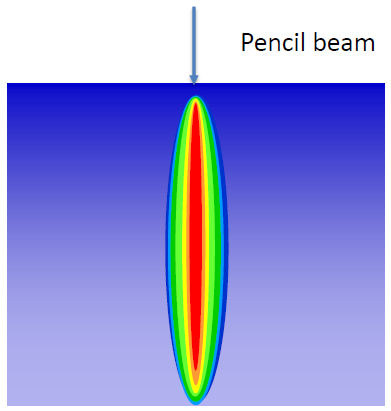
\includegraphics[width=.4\textwidth]{./cap1/electr_pencil.png}$\qquad$
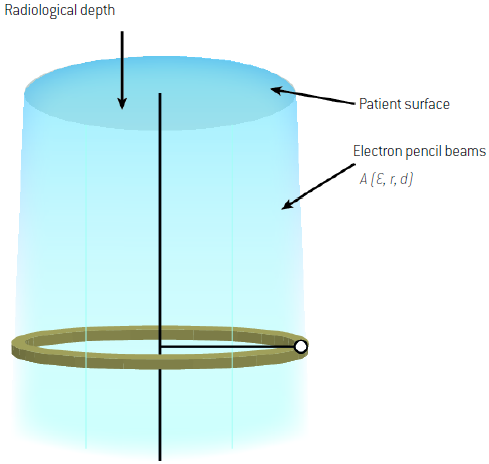
\includegraphics[width=.45\textwidth]{./cap1/electr_pencil_b.png}
\caption{Sinistra: kernel di deposizione di tipo \textit{pencil-beam}. Destra: figura schematica che mostra la simmetria cilindrica nel calcolo della dose quando si utilizza un kernel di tipo \textit{pencil-beam}.}
\label{fig:electr_pencil}
\end{figure}


Questo tipo di algoritmo è denominato \textit{pencil-beam} e rappresenta una versione semplificata del collapsed-cone.\\
L'equazione che permette il calcolo della dose è analoga alla \eqref{eq:superp} ed è facilmente calcolabile in coordinate cilindiriche:
\begin{equation}
\label{eq:electr_superp}
D(d) = 2\pi \iint_{E,V} \Psi(r,d,E)\, s(r,d,E)\, r\de r \de E
\end{equation}

L'Eq.\eqref{eq:electr_superp} è implementata all'interno di RayStation in maniera analoga al caso dei fotoni che riassumiamo in maniera schematica:
\begin{itemize}
\item I kernel \textit{pencil-beam} sono pre-calcolati con un modello Monte Carlo (software EGSnrc).
\item Viene utilizzato un modello a due sorgenti per calcolare la fluenza di energia in assenza del paziente.
\item Viene calcolata la distribuzione di TERMA utilizzando la formula della perdita di energia per ionizzazione di Bethe-Bloch per gli elettroni nella materia \cite{RaySearchLaboratories2014}.
\item Vengono applicati i kernel \textit{pencil-beam} per modellizzare lo scatter laterale degli elettroni.
\end{itemize}

Nella Fig.\ref{fig:electr_enloss} è mostrata la distribuzione di dose dovuta agli elettroni di contaminazione calcolata su una CT di un paziente. Questa dose viene sommata alla dose dovuta ai fotoni calcolata con l'algoritmo collapsed-cone. 
















\chapter{Modellizzazione f{}isica del LINAC nel TPS RayStation}
\minitoc
\textsf{In questo capitolo verranno introdotti i concetti di dosimetria di base di un acceleratore lineare. A partire da queste misure, viene costruito un modello dosimetrico del LINAC all'interno del TPS. Viene poi discussa l'accuratezza richiesta per un calcolo dosimetrico al variare della tecnica di erogazione assieme alle scelte e i metodi adottati per raggiungerla. Infine vengono presentate le verifiche pre-cliniche propedeutiche all'immissione del TPS nella routine clinica.}



\section{Dosimetria di base di un LINAC}
Le misure necessarie a costruire un modello dosimetrico di un LINAC consistono in curve di dosimetria relativa e misure puntuali di dose (assoluta e relativa).\\
Storicamente, queste misurazioni vengono effettuate con detector a camera a ionizzazione\footnote{La camera a ionizzazione è un rivelatore di radiazione ionizzante a gas. \`E costituita da due elettrodi che racchiudono un certo volume di aria. Al passaggio della radiazione, l'aria viene ionizzata e libera coppie di ioni. Grazie ad un campo elettrico applicato tra i due elettrodi gli ioni migrano fino a giungere sull'anodo, provocando un segnale in corrente rivelabile.}. Tuttavia, con l'avvento delle tecniche di radioterapia avanzata (es. intensità modulata o stereotassi), sono stati introdotti una molteplicità di detector di nuova generazione specie per soddisfare le esigenze di accuratezza di misura per piccoli campi di irradiazione\footnote{Un campo quadrato è ritenuto \textit{piccolo} se inferiore a $4$x$4$ cm$^2$ \cite{Das2008}.}. Nella sezione seguente verranno presentati i concetti classici di dosimetria di un LINAC propedeutici alla modellizzazione di un TPS. Ci si soffermerà dapprima alla tecnica di irradiazione denominata \textit{radioterapia conformazionale}\footnote{La radioterapia conformazionale o 3D-CRT è una tecnica di irradiazione che  fa impiego di fasci di irradiazione collimati sul target per i quali la pianificazione ed il calcolo della dose vengono effettuati su uno studio di tomografia computerizzata del paziente.}. Le problematiche relative alla dosimetria dei piccoli campi e alle tecniche di irradiazione avanzata verranno discusse a seguire. 

\subsection{Dosimetria relativa}
\label{sec:dos_rel}
Per dosimetria relativa si intende tutta una serie di misure della dose non in termini assoluti (in Gray) ma in percentuale rispetto a uno o più riferimenti. In particolare, le misure di dosimetria relativa necessarie alla modellizzazione di un TPS generico possono essere suddivise in tre catagorie:
\begin{itemize}
\item Curve di dose-profondità (PDD).
\item Profili di dose.
\item Output factor.
\end{itemize}
Queste misure vengono effettuate in un fantoccio cubico riempito di acqua (materiale più simile ai tessuti umani) dotato di un carrello motorizzato su cui viene montata la camera a ionizzazione che effettua le misure di dose (vedi Fig.\ref{fig:wphant}).
\begin{figure}[!t]
\centering
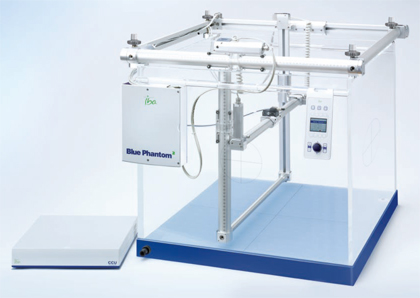
\includegraphics[width=.45\textwidth]{./cap2/wphant.jpg}
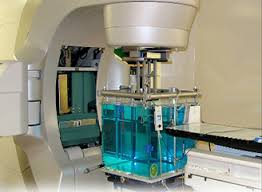
\includegraphics[width=.45\textwidth]{./cap2/wphant_pos.jpg}
\caption{Fantoccio per le misure di dosimetria assoluta e relativa (foto e suo posizionamento rispetto al LINAC).}
\label{fig:wphant}
\end{figure}

Le curve di dose-profondità si ottengono muovendo il detector lungo l'asse centrale del fascio (in direzione verticale) con un certo step (tipicamente 1 mm).\\
Per ogni punto, la camera a ionizzazione registra una certa dose che viene normalizzata rispetto ad una lettura di riferimento (tipicamente la lettura corrispondente alla massima dose lungo la verticale).

I profili di dose si ottengono in maniera analoga muovendo il detector in piani perpendicolari all'asse del fascio. Tipicamente vengono acquisiti profili di dose lungo due assi perpendicolari denominati \textit{inline} e \textit{crossline}\footnote{Considerando un paziente supino con la testa verso il gantry del LINAC, l'asse \textit{inline} corrisponde alla direzione testa-piedi e l'asse \textit{cross-line} alla direzione sinistra-destra.} a varie profondità.\\
\begin{figure}[!t]
\centering
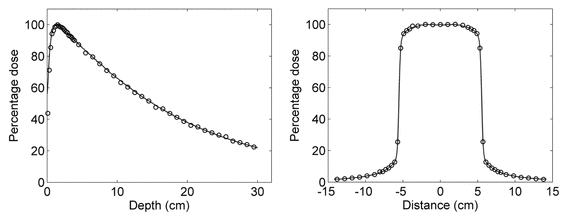
\includegraphics[width=\textwidth]{./cap2/pdd_prof.png}\\
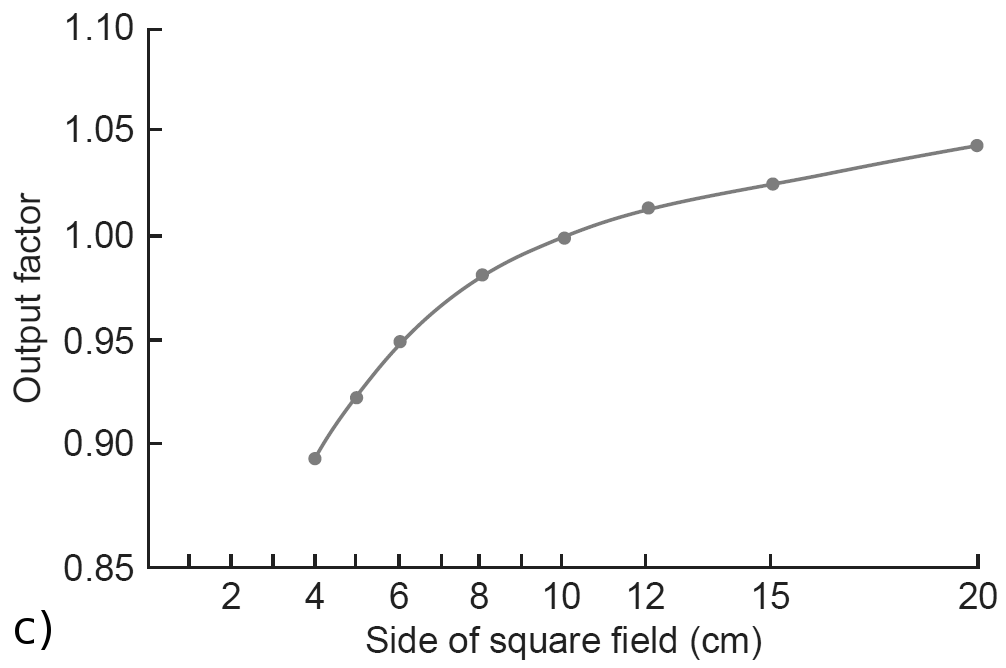
\includegraphics[width=.5\textwidth]{./cap2/of.png}
\caption{Tipici andamenti delle misure di dosimetria relativa: curva dose-profondità (PDD) (a); profilo di dose (b); output factor (c).}
\label{fig:pdd_prof}
\end{figure}
Nella Fig.\ref{fig:pdd_prof} è possibile visualizzare gli andamenti tipici di una curva di dose-profondità e di un profilo di dose.

Nelle curve di dose-profondità è possibile distinguere tre zone:
\begin{itemize}
\item \textit{Zona di build-up:} la prima parte ascendente della PDD in cui avvengono le prime interazioni dei fotoni nel mezzo. Gli elettroni vengono messi in moto da queste interazioni primarie e depositano energia più avanti con i processi descritti nel capitolo 1. Se non vi fossero gli elettroni di contaminazione del fascio, la dose nei primi millimetri di materiale sarebbe quasi nulla\footnote{Questo effetto è considerato un beneficio in radioterapia ed è noto anche come \textit{skin-sparing-effect.}}.
\item \textit{Massimo della PDD:} all'aumentare della profondità, aumenta la produzione di particelle secondarie fino ad arrivare ad un equilibrio noto come equilibrio di particelle cariche (CPE). In queste condizioni il numero di particelle cariche uscenti da un volume è uguale al numero di particelle entranti in esso.
\item \textit{Parte discendente della PDD:} aumentando ulteriormente la profondità di tessuto attraversato, il fascio primario decresce esponenzialmente e conseguentemente anche la dose segue questo andamento.
\end{itemize}

Una distinzione simile può essere fatta per i profili di dose:
\begin{itemize}
\item \textit{Zona in-field:} la parte centrale del profilo compresa in un range di dose che va dal 100\% all'80\% rispetto alla massima dose registrata.
\item \textit{Penombra:} ai bordi del campo la dose scende rapidamente a causa della schermatura dei collimatori. La penombra è definita come la porzione di spazio compresa tra l'80\% e il 20\% della dose massima.
\item \textit{Zona out-of-field:} al di fuori delle dimensioni geometriche del campo sono presenti delle code a bassa dose che si estendono lateralmente anche al di sotto della zona schermata dai collimatori. Questa dose residua è dovuta ai processi di scatter della radiazione primaria e di quella secondaria. Corrisponde alla zona al di sotto del 20\% della dose massima del profilo.
\end{itemize}

Come vedremo in seguito, l'accuratezza di un calcolo dosimetrico tramite TPS viene valutata per ognuna delle zone sopra citate, con diversi livelli di tolleranza. 

Assieme alle PDD e ai profili, viene effettuata una misura di dose puntuale al variare delle dimensioni del campo di irradiazione (\textit{output factor}). In particolare, viene registrata la lettura di dose al centro del fascio ad una certa profondità (tipicamente 10 cm) e per una dimensione di campo di riferimento (10$x$10 cm$^2$). Viene quindi ripetuta la lettura al variare delle dimensioni del campo di irradiazione, normalizzando il tutto alla lettura di riferimento. L'andamento tipico che si ottiene per un fascio di fotoni è riportato nella Fig.\ref{fig:pdd_prof}. L'output factor aumenta all'aumentare delle dimensioni del campo e ciò è dovuto principalmente ai processi di scatter che assumono più rilevanza e contribuiscono ad incrementare la lettura di dose al centro.

\subsection{Dosimetria assoluta}
\label{sec:dose_ass}
Una volta concluse le misure di dosimetria relativa, è necessario effettuare una misura di dose assoluta che permette di trasformare tutte le curve percentuali in curve di dose reale (in unità di Gray). La misurazione della dose assoluta è regolata da specifici protocolli redatti da organizzazioni internazionali come l'AAPM (America) \cite{Almond1999} e la International Atomic Energy Agency (IAEA) (Europa) \cite{Andreo2006}.\\
Per il commissioning dell'acceleratore oggetto di questa tesi è stato seguito il protocollo IAEA TRS-398 secondo cui la dose assoluta può essere ottenuta con la seguente formula:
\begin{equation}
D = M\,N_{d,w}\,k_{Q,Q_0}\,k_{TP}\,k_h\,k_{pol}\,k_{sat}
\end{equation}
dove:
\begin{description}
\item[$M:$] lettura della ionizzazione in Coulomb (effettuata con la camera a ionizzazione).
\item[$N_{d,w}:$] coefficiente di taratura della camera a ionizzazione che converte il valore in Coulomb nella dose in Gray in acqua per un fascio di riferimento (solitamente generato da una sorgente di Co-60).
\item[$k_{Q,Q_0}:$] fattore correttivo che tiene conto della diversa distribuzione energetica (qualità) di un fascio clinico generato da un LINAC rispetto al Co-60 e che dipende dalla specifica camera a ionizzazione.
\item[$k_{TP}:$] fattore correttivo che tiene conto della diversa temperatura e pressione durante la misura rispetto alle condizioni di riferimento.
\item[$k_{H}:$] fattore correttivo che tiene conto della diversa umidità durante la misura rispetto alle condizioni di riferimento.
\item[$k_{pol}:$] fattore che tiene conto della diversa lettura di carica che si ottiene con una camera a ionizzazione applicando un voltaggio positivo o negativo tra i due elettrodi.
\item[$k_{sat}:$] fattore che tiene conto degli effetti di ricombinazione delle cariche all'interno del volume di aria della camera a ionizzazione.
\end{description}
I suddetti fattori correttivi sono riportati in forma tabellare oppure si ricavano da misurazioni. Una discussione approfondita della misura di dose assoluta esula dagli scopi di questa tesi per cui si rimanda al protocollo \cite{Andreo2006}.

\subsection{Misure richieste per la modellizzazione del TPS RayStation}
Come già citato nelle sezioni precedenti, le misure necessarie a modellizzare un LINAC all'interno del TPS RayStation consistono in curve dose-profondità, profili di dose a varie profondità, output factor e una misura di dose assoluta per ogni qualità del fascio da modellizzare.\\
Nella Tab.\ref{tab:meas} sono indicate le dimensioni di campo per le quali è consigliato acquisire PDD, profili e  output factor.
\begin{table}
\arrstr{1.2}
\begin{tabular}{@{}ccc@{}}
\toprule
Campi consigliati (cm$^2$) & Campi opzionali (cm$^2$) & Profondità profili (cm)\\
\midrule
2x2 & 1x1 & 1.5\\
3x3 & 4x4 & 3.0\\
5x5 & 6x6 & 5.0\\
10x10 & 7x7 & 10.0\\
15x15 & 8x8 & 15.0\\
20x20 & 9x9 & 20.0\\
30x30 & 12x12 & \\
40x40 & 25x25 & \\
\bottomrule
\end{tabular}
\caption{Misure consigliate e opzionali per le curve di PDD, profili e output factor.}
\label{tab:meas}
\end{table}
Queste misure costituiscono solo un'indicazione e possono essere estese o ridotte a seconda della tecnica di irradiazione e dell'accuratezza che si vuole raggiungere nel calcolo della dose.

\section{Accuratezza nel calcolo della dose con TPS}
\subsection{Accuratezza richiesta per la 3D-CRT}
\label{sec:accu_3D}
L'accuratezza richiesta per il calcolo della dose in radioterapia conformazionale si basa su criteri stabiliti agli inizi degli anni duemila da Van Dyk et al. e Venselaar et al. \cite{Dyk1993,Venselaar2001}. Da questi due lavori pioneristici, sono scaturite un certo numero di raccomandazioni da parte di organi internazionali (AAPM, ESTRO, IAEA) che hanno stabilito i limiti di accettabilità per la precisione di un calcolo di dose tramite TPS \cite{Fraass1998,Mijnheer2004,IAEA430}.\\
Il protocollo adottato per gli scopi di questa tesi è il \textit{booklet no.7} della \textit{European SocieTy for Radiotherapy \& Oncology} (ESTRO). 
\begin{figure}[!t]
\centering
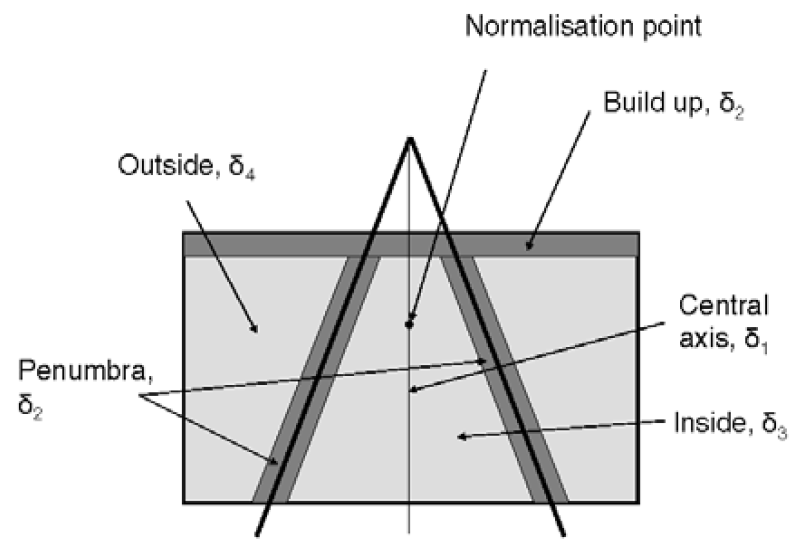
\includegraphics[width=.65\textwidth]{./cap2/Accuracy_zones.png}\\\vspace{.3cm}
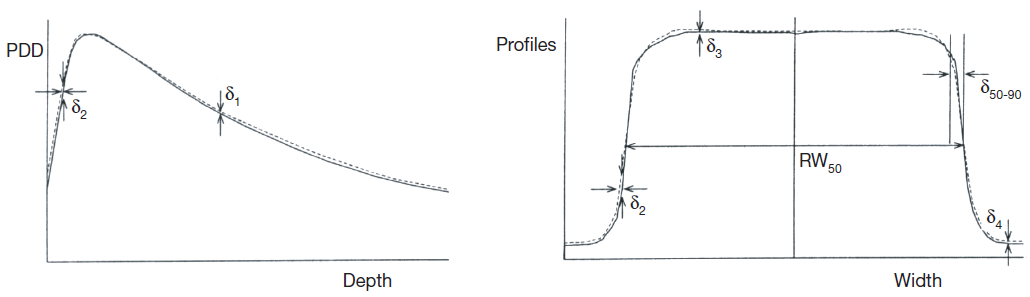
\includegraphics[width=\textwidth]{./cap2/Accuracy_pdd_prof.png}
\caption{(a) suddivisione delle varie zone di interesse su cui valutare l'accuratezza del calcolo di dose con la tolleranza specifica $\delta_i$, $i\in[1,4]$. (b) tolleranze visualizzate sulle varie zone in interesse per una PDD e un profilo di dose. I valori numerici delle tolleranze sono indicati nella Tab.\ref{tab:tol}}
\label{fig:accuracy_zones}
\end{figure}

\begin{table}
\centering
\includegraphics[width=\textwidth]{./cap2/accuracy_tol.png}
\caption{Livelli di tolleranza per le varie zone indicate nella Fig.\ref{fig:accuracy_zones} e per vari livelli di complessità del calcolo. Riprodotta da \cite{Mijnheer2004}.}
\label{tab:tol}
\end{table}
Nella radioterapia tradizionale 3D-CRT è sufficiente effettuare misure di PDD, profili e output factor per dimensioni di campo che vanno da 5$x$5 cm$^2$ a 40$x$40 cm$^2$. Per tali dimensioni di campo è possibile utilizzare detector a camera a ionizzazione senza incorrere nelle problematiche che riguardano i piccoli campi di irradiazione ($< 4x4\,$cm$^2$) \cite{Das2008}. Un TPS per 3D-CRT deve riprodurre le misure effettuate con delle accuratezze variabili a seconda della regione di valutazione. Nella Fig.\ref{fig:accuracy_zones} è riportata la distinzione  nelle varie zone di interesse di un fascio di irradiazione assieme alle tolleranze applicabili ad ognuna di esse. I valori numerici sono indicati nel booklet ESTRO no.7 e sono riportati nella Tab.\ref{tab:tol}.\\
I criteri di accettabilità del calcolo vengono applicati valutando due principali quantità:

\begin{description}

\item[Differenza di dose misurata-calcolata:] questa quantità è calcolata con la formula:
\begin{equation}
\delta = 100\% \times \frac{D_{calc} - D_{meas}}{D_{N}}
\end{equation}
dove $D_{calc}$ e $D_{meas}$ rappresentano le dosi misurate e calcolate in un punto e $D_N$ rappresenta la dose di normalizzazione della differenza. Secondo le indicazioni ESTRO, $D_N$ è data dalla \textit{dose misurata locale} al punto di valutazione $D_{meas}$ nelle zone ad alta dose mentre è data dalla \textit{dose misurata a centro asse}  $D_{CAX,meas}$ nelle zone a bassa dose (es. code dei profili).\\
La valutazione in differenza di dose è adatta per le zone in cui si ha un basso gradiente ($\delta D < 3\%\,$mm$^{-1}$) (es. parte discendente della PDD e parte in-field e out-field dei profili).

\item[Distanza di accordo:] questa quantità rappresenta la minima distanza tra un punto individuato dal vettore $\vec{r}_{meas}$ dove è stata misurata una certa dose e tutti i punti $\vec{r}_{calc}$ per cui la dose calcolata è  uguale a quella misurata.
\begin{equation}
DTA = \min_{\vec{r}_{calc}} \left|\vec{r}_{meas} - \vec{r}_{calc}\right|
\end{equation}
La distanza di accordo è consigliata dal protocollo ESTRO per le valutazioni di accettabilità delle zone ad alto gradiente ($\delta D > 3\%\,$mm$^{-1}$) (es. build-up delle PDD e penombre dei profili).
\end{description}

I valori di tolleranza in differenza di dose e DTA (Tab.\ref{tab:tol}) oscillano tra il 2\% - 2 mm, per geometrie semplici, (es. campo quadrato, fantoccio omogeneo) e il 5\% - 3 mm per i calcoli più complessi (es. dose fuori campo in condizioni di disomogeneità e asimmetria).\\
Una metodologia conveniente per eseguire una valutazione combinata dei criteri di differenza di dose e distanza di accordo è stata sviluppata da Low et al. \cite{Low1998}. Essa si basa sul dividere queste due quantità con le rispettive tolleranze e sommarle per costruire un indice adimensionale denominato \textit{$gamma$-index} (lettera greca per `c' che sta per `combined-index'):
\begin{equation}
\gamma = \min_{\vec{r}_{c}} \sqrt{\frac{|\vec{r}_{m}-\vec{r}_{c}|^2}{\Delta r}   + \frac{\left[D_{m}(\vec{r}_{m})-D_{c}(\vec{r}_{c})\right]^2}{\Delta D} }
\label{eq:gamma}
\end{equation}
dove i pedici `$m$' e `$c$' indicano `misurato' e `calcolato' e $\Delta r$ e $\Delta D$ costituiscono le tolleranze rispettivamente per la distanza di accordo e la differenza di dose. Il criterio di accettabilità viene soddisfatto nel punto di interesse se risulta $\gamma < 1$.

\begin{figure}[!t]
\centering
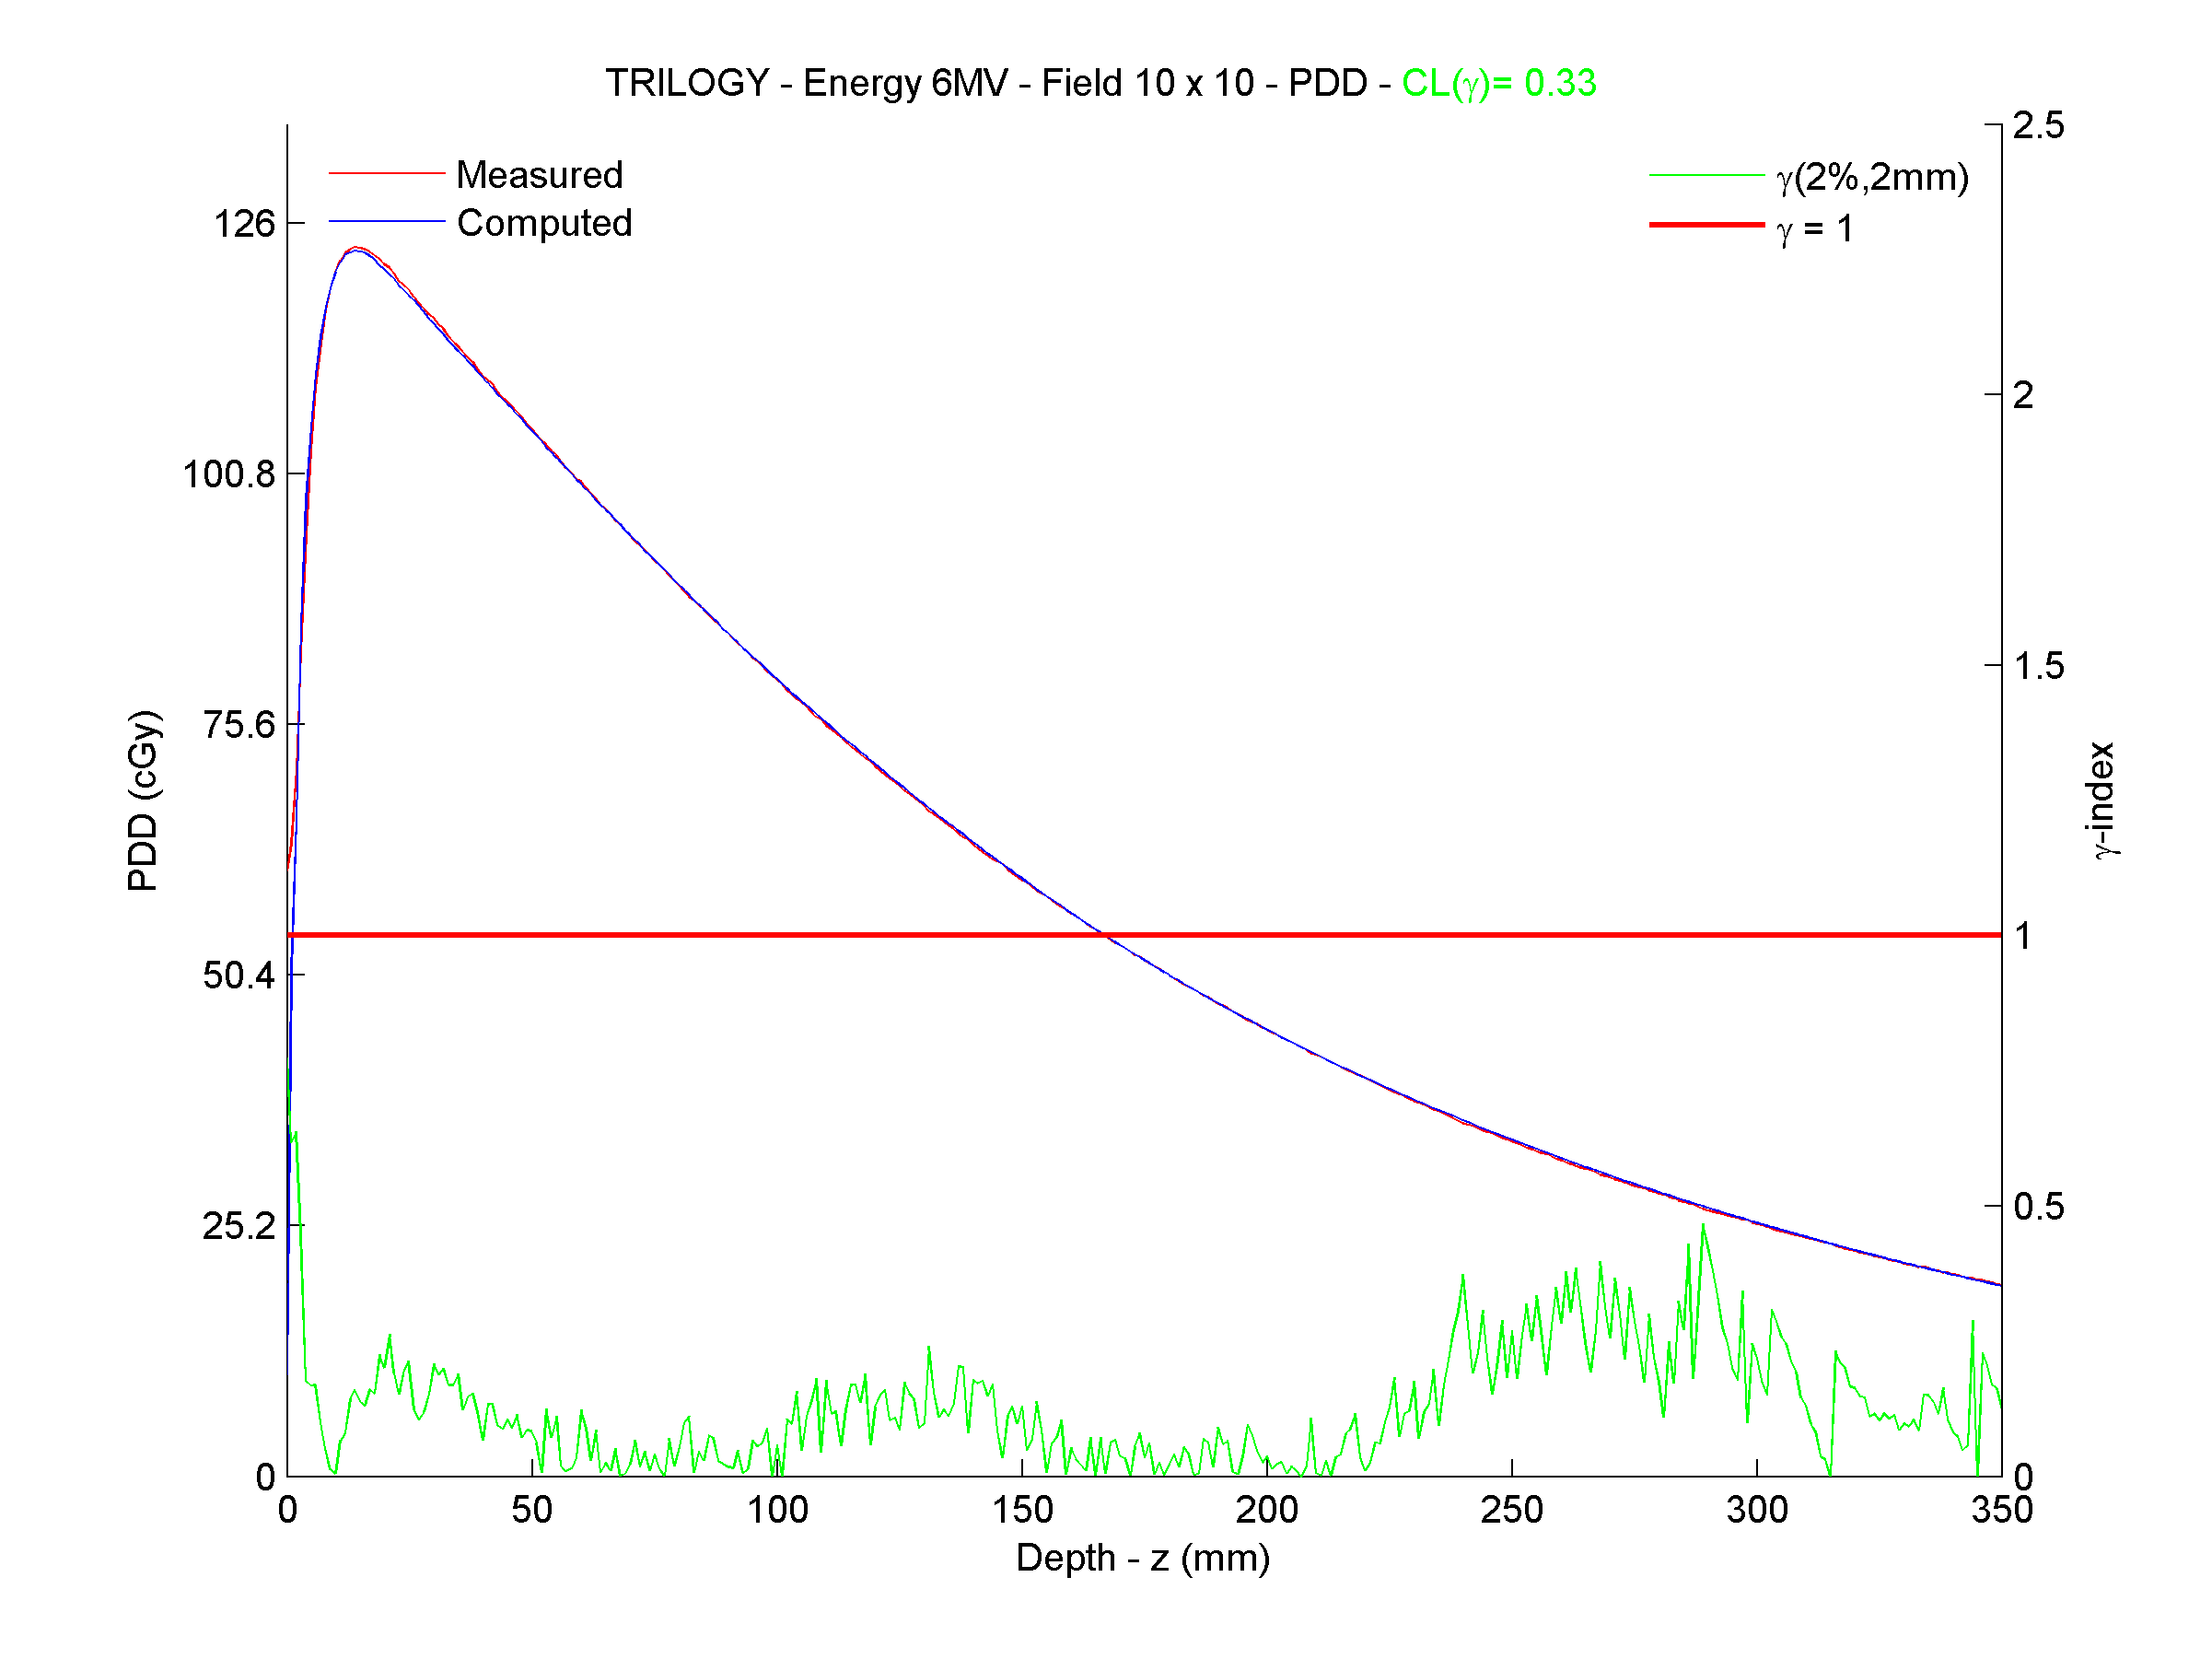
\includegraphics[width=.9\textwidth]{./cap2/pdd10x10.png}
\caption{Confronto tra una PDD misurata e calcolata con il criterio del livello di confidenza dell'indice $\gamma$. Dalla distribuzione dei valori dell'indice $\gamma$ vengono calcolate la media e la deviazione standard e applicata la formula di Venselaar \eqref{eq:clgamma} per il calcolo del livello di confidenza dell'indice $\gamma$. Nel caso indicato in figura $CL(\gamma)=0.33$}
\label{fig:gamma10x10}
\end{figure}

Tuttavia, le raccomandazioni ESTRO sconsigliano di valutare l'accettabilità del calcolo di un profilo o PDD con un criterio puntuale bensì, di utilizzare un criterio che consideri tutti i punti della curva di dose. Questo criterio è detto livello di confidenza dell'indice $\gamma$ ed è stato introdotto da Venselaar et al.\cite{Venselaar2001}:
\begin{equation}
CL(\gamma) = \bar{\gamma} + 1.5\,\sigma(\gamma)
\label{eq:clgamma}
\end{equation}
dove $\bar{\gamma}$ è la media di tutti i valori dell'indice $\gamma$ calcolati sulla curva di dose e $\sigma(\gamma)$ è la loro deviazione standard (vedi Fig.\ref{fig:gamma10x10}).
Il confronto tra una curva di dose misurata e la corrispettiva calcolata risulta in tolleranza se il livello di confidenza dell'indice $\gamma$ risulta minore di 1 ($CL(\gamma) < 1$).


\subsection{Accuratezza richiesta per le tecniche avanzate (IMRT e VMAT). La problematica dei piccoli campi di irradiazione}
\label{sec:accu_spec}
Per tecniche `avanzate' si intendono maggiormente le tecniche ad intensità modulata (IMRT). A differenza della 3D-CRT, queste tecniche realizzano una distribuzione di dose modulata all'interno del medesimo fascio di irradiazione con il beneficio di ottenere una maggiore conformazione della dose attorno al bersaglio \cite{ICRU2010} (Fig.\ref{fig:3D_IMRT}).\\
\begin{figure}
\centering
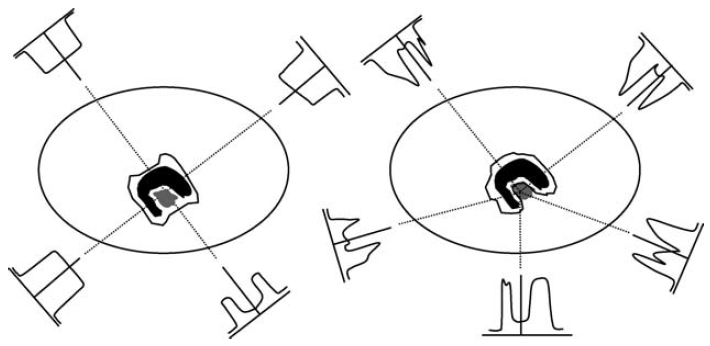
\includegraphics[width=\textwidth]{./cap2/3D_IMRT.png}
\caption{Differenza tra fasci di irradiazione conformati (3D-CRT) e fasci erogati in tecnica ad intensità modulata (IMRT).}
\label{fig:3D_IMRT}
\end{figure}
La modulazione della dose può essere realizzata in modalità \textit{step-and-shoot} (SMLC), ossia sommando una serie di fasci caratterizzati da diverse collimazioni (segmenti) \cite{Bortfeld1994}, oppure in modalità \textit{dinamica}  (DMLC), che realizza la modulazione muovendo dinamicamente il multi-leaf-collimator \cite{LING1996}. Più recentemente, è stata introdotta un'ulteriore modalità detta \textit{arcoterapia volumetrica} (VMAT) che realizza una distribuzione di dose modulata collimando il fascio durante la rotazione del gantry e modificando contemporaneamente il rateo di dose \cite{Otto2008}.\\
La caratteristica che accomuna tutte queste tecniche è il largo uso di campi di piccole dimensioni (i.e. $<4x4$ cm$^2$ \cite{Das2008}). Per questo motivo, per il commissioning di un TPS dedicato alla pianificazione di trattamenti IMRT o VMAT, è necessario estendere le misure di PDD, profili e output factor ai campi piccoli ed anche rivalutare l'accuratezza tollerabile per un calcolo dosimetrico.

La dosimetria dei piccoli campi di irradiazione presenta varie criticità \cite{Das2008} tra cui:
\begin{itemize}
\item Mancanza di equilibrio di particelle cariche (CPE) laterale.
\begin{itemize}
\item[-] Questo effetto si realizza quando le dimensioni del campo sono comparabili con il range medio degli elettroni secondari. Per energie del fascio primario minori di $10\,$MV, la condizione CPE non è soddisfatta per dimensioni di campo al di sotto di $3x3\,$cm$^2$.
\end{itemize}
\item Apertura dei collimatori comparabili con la dimensioni proiettate della sorgente.
\begin{itemize}
\item[-] Questo crea un doppio effetto che consiste in una forte riduzione della dose sull'asse centrale del fascio assieme ad una modificazione della forma del profilo (forma ogivale e allargamento della penombra) (vedi Fig.\ref{fig:small_eff}a).
\end{itemize}
\item Dimensioni dei detector comuni comparabili con le dimensioni del campo.
\begin{itemize}
\item[-] Ciò può portare ad un effetto di \textit{volume averaging} indicato nella Fig.\ref{fig:small_eff}b che si traduce in una sottostima del massimo della dose al centro e ad una modificazione delle penombre.
\end{itemize}
\end{itemize}
\begin{figure}[!t]
\centering
a)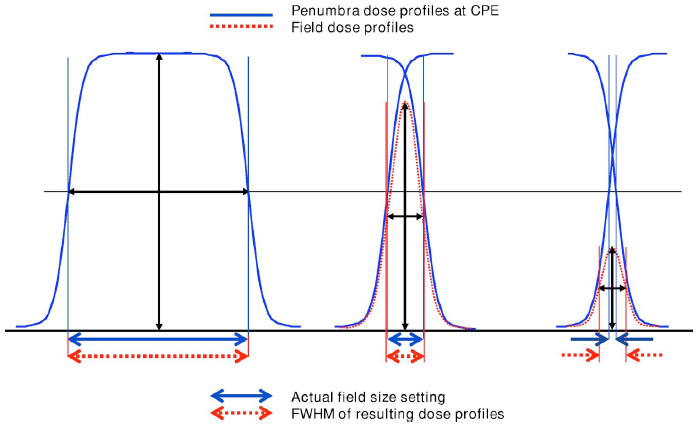
\includegraphics[width=.7\textwidth]{./cap2/small_eff1.png}
b)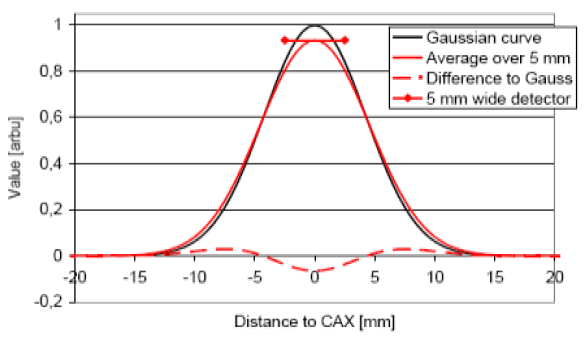
\includegraphics[width=.7\textwidth]{./cap2/small_eff2.png}
\caption{(a) la sovrapposizione delle penombre dei collimatori (legate alle dimensioni della sorgente primaria) porta ad una modificazione della forma del profilo di dose (forma ogivale e penombre allargate) assieme ad una forte riduzione della dose al centro. (b) un detector di dimensioni comparabili con le dimensioni del profilo può portare ad una sottostima della dose a causa dell'effetto di \textit{volume averaging}.}
\label{fig:small_eff}
\end{figure}

Queste condizioni sono lontane dalle tipiche condizioni di riferimento dettate dai consolidati protocolli di dosimetria \cite{Almond1999,Andreo2006} pensati per la 3D-CRT. Per minimizzare le incertezze che derivano da queste criticità sui piccoli campi, negli anni sono stati sviluppati una serie di detector di nuova generazione quali micro-camere a ionizzazione, rivelatori a semiconduttore, rivelatori a scintillazione etc., con l'intento comune di ridurre le dimensioni del volume sensibile, preservando le caratteristiche di affidabilità di un detector comunemente impiegato per 3D-CRT (linearità, indipendenza dall'energia, indipendenza dal rateo di dose\ldots).\\
Una estensiva review dei detector, delle loro problematiche e delle tecniche di misura consigliate per piccoli campi è stata recentemente pubblicata dal task group (TG) 120 dell'associazione americana dei fisici medici (AAPM) \cite{Low2011}. Sulla base dei risultati passati in rassegna dal TG-120, la comunità scientifica dell'AAPM e della IAEA è al lavoro congiuntamente per aggiornare i classici protocolli di dosimetria ed emettere delle nuove raccomandazioni che permettano una misura accurata della dose anche in presenza delle succitate criticità. In conclusione, una parte rilevante dell'accuratezza richiesta nel calcolo della dose in IMRT e VMAT è legata all'accuratezza con cui viene effettuata la dosimetria dei piccoli campi in quanto parti rilevanti della modellizzazione del TPS si basano su queste misurazioni.

Accanto all'accuratezza richiesta nell'acquisizione delle misure, vi è l'accuratezza del calcolo del dose da considerare. Le indicazioni relative all'accuratezza di un TPS per IMRT sono state studiate dal task group 119 della AAPM \cite{Ezzell2009}. Il report suggerisce di conservare ed estendere ai campi piccoli le tolleranze per 3D-CRT riportate in Tab.\ref{tab:tol} e di revisionare la formula di Venselaar \eqref{eq:clgamma}:
\begin{equation}
CL(\gamma)_{\text{IMRT}} = \bar{\gamma} + 1.96\,\sigma(\gamma)
\end{equation}
Oltre ad indicare i criteri di accettazione per le curve di dose, il TG-119 riporta anche delle tolleranze di accettabilità per una serie di test che simulano delle comuni situazioni cliniche e che sono stati presi in considerazione nelle fasi finali del commissioning del TPS. 

\section[Scelte adottate per le misure]{Scelte adottate per le misure\protect\footnote{Le misure e la conseguente modellizzazione del LINAC sono presentate in questo lavoro per un fascio di energia nominale pari a $6\,$MV. Il processo è stato ripetuto per un'altra energia pari a $15\,$MV ma non verrà discusso in quanto analogo.}}


\subsection{PDD e Profili di dose}
Il LINAC oggetto di questa tesi è un modello Trilogy\textsuperscript{\textcopyright} prodotto dalla Varian Medical Systems. Esso è progettato per poter erogare trattamenti radioterapici in tecnica conformazionale o ad intensità modulata (IMRT) step-and-shoot e dinamica fino ad una dimensione di campo massima $40x40\,$cm$^2$. \`E inoltre in grado di erogare trattamenti volumetrici ad arco con intensità e rateo di dose modulati (VMAT) fino ad una dimensione di campo massima $30x30\,$cm$^2$. Oltre a queste caratteristiche legate all'erogazione, è inoltre capace di effettuare uno studio di tomografia computerizzata del paziente prima del trattamento, in modo da verificare in tre dimensioni l'accurata collocazione sia del paziente in sé sia dei suoi organi interni, rispetto alle posizioni pianificate.

La distanza tra la sorgente di radiazione e l'acqua contenuta del fantoccio di misura (SSD) è stata posta a $90\,$cm sulle basi delle raccomandazioni della ditta ed anche del report 106 dell'AAPM \cite{Das2008a} che indica $90\,$cm come la SSD più vicina alle condizioni dei trattamenti più comuni.

Seguendo le linee guida AAPM TG-120 citate nella sezione precedente \cite{Low2011} e tenendo conto delle raccomandazioni della ditta produttrice del TPS (Tab.\ref{tab:meas}), le scelte effettuate per le misure di PDD e profili di dose sono state le seguenti:
\begin{itemize}
\item Dimensioni di campo (in cm$^2$) $5x5$, $7x7$, $10x10$, $15x15$, $20x20$, $30x30$ e $40x40$ misurate con detector a camera a ionizzazione modello CC13 prodotto dalla IBA Dosimetry (volume attivo: $0.13\,$cm$^3$).
\item Dimensioni di campo (in cm$^2$) $1x1$, $2x2$, $3x3$ e $4x4$ misurate con detector a semiconduttore (diodo) modello PFD prodotto dalla IBA Dosimtery (volume attivo: $0.09\,$mm$^3$).
\end{itemize}
Queste scelte ricalcano le raccomandazioni dei consolidati protocolli di dosimetria per quanto riguarda l'utilizzo della camera a ionizzazione per i campi al di sopra di $4x4\,$cm$^2$ mentre considerano le nuove evidenze sperimentali \cite{Das2008a,Low2011} riguardo l'utilizzo di detector di piccole dimensioni per i campi al di sotto di $5x5\,$cm$^2$. Nello specifico, in Fig.\ref{fig:pen_of}a vengono confrontate le penombre dei profili di dose misurate con vari detector tra cui quelli utilizzati nell'ambito di questo lavoro.
\begin{figure}[!t]
\centering
a)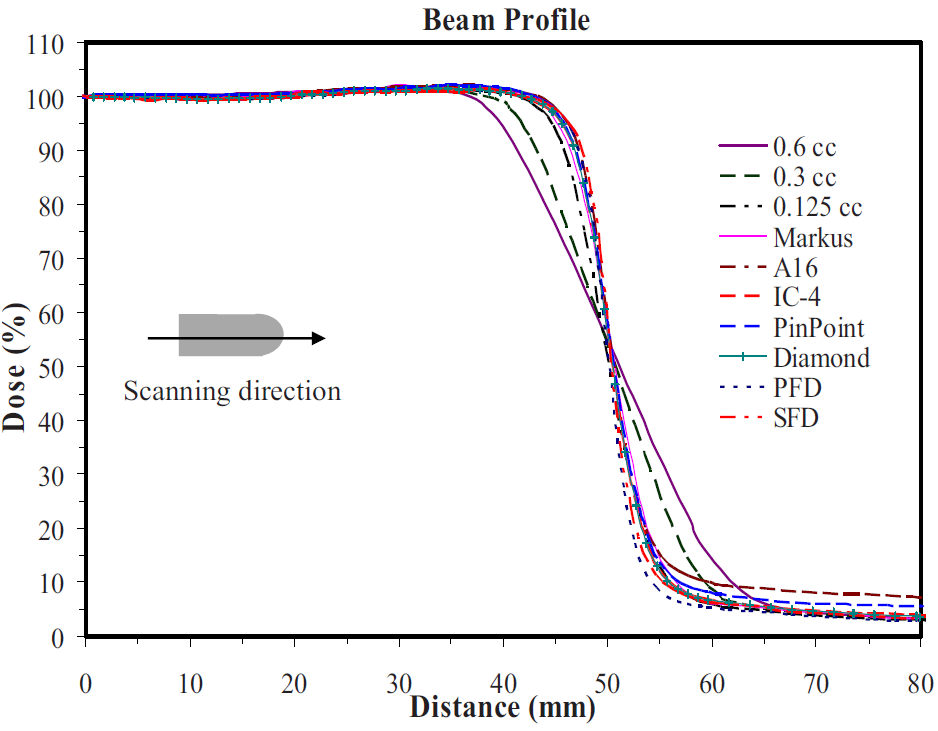
\includegraphics[width=.75\textwidth]{./cap2/pen_smear.png}\\
b)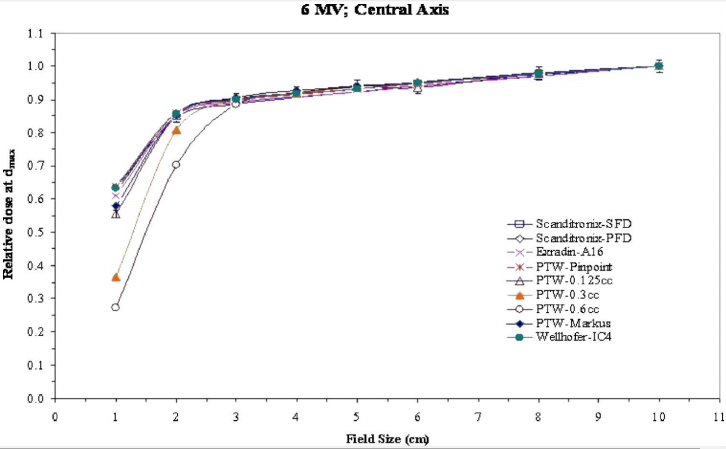
\includegraphics[width=.75\textwidth]{./cap2/OF_uncert.png}
\caption{(a) Effetto di smussamento della penombra dei profili dovuto al volume esteso delle camere a ionizzazione confrontato con scansioni effettuate con detector di dimensioni ridotte \cite{Das2008a}. (b) misura degli output factor a piccoli campi a seconda del detector impiegato\cite{Das2008}.}
\label{fig:pen_of}
\end{figure}
Si può notare come le camere a ionizzazione con estesi volumi sensibili ($0.6\,$cc e $0.3\,$cc) portino ad una sovrastima della penombra a causa dell'effetto di volume-averaging. L'effetto è tanto più trascurabile quanto più viene diminuita la dimensione del detector (es. micro-camera a ionizzazione con volume sensibile di $0.125\,$cc oppure detector a semiconduttore come PFD e SFD). L'accurata misura delle penombre, è di cruciale importanza in quanto vedremo che la modellizzazione delle dimensioni della sorgente primaria è tanto più precisa quanto più lo sono le misure di penombra dei campi di piccole dimensioni.

\subsection{Output factor}
Come già introdotto nella Sez.\ref{sec:dos_rel}, gli output factor (OF) costituiscono misure di punto relative e si determinano per ogni dimensione campo di cui sono state acquisite le PDD e i profili con la formula:
\begin{equation}
\label{eq:OF}
OF(XxY)=\frac{D(XxY)}{D(10x10)}
\end{equation}
dove $D(XxY)$ è la lettura di dose per un campo di dimensioni $XxY\,$cm$^2$ e $D(10x10)$ è la lettura di dose per il campo di riferimento ($10x10\,$cm$^2$). Tutte le letture di dose sono state effettuate a centro asse e a $10\,$cm di profondità\footnote{In dosimetria relativa il termine `dose' è utilizzato come sinonimo di carica integrata raccolta dal rivelatore per un fissato intervallo di tempo.  Ciò non è da confondere con la `dose' in dosimetria assoluta che comporta un processo di misura più complesso (Sez.\ref{sec:dose_ass}).}.

Seguendo le indicazioni delle ditta produttrice del TPS \cite{RaySearchLaboratories2014}, gli OF sono stati misurati per ogni dimensione di campo con il medesimo detector utilizzato per le misure di PDD e profili di dose. Mentre per i campi al di sopra di $4x4\,$cm$^2$ è stata impiegata una camera a ionizzazione secondo una procedura consolidata per la 3D-CRT \cite{Andreo2006}, il rivelatore a semiconduttore PFD utilizzato per i campi piccoli può presentare delle criticità. Varie evidenze scientifiche riassunte dall'AAPM TG-120 \cite{Low2011} hanno dimostrato che la classe di dosimetri basata su semiconduttore al silicio tende a sovrastimare la lettura di dose \cite{Low2011}. Ciò è dovuto al più alto numero atomico del silicio rispetto al numero atomico medio dell'acqua che comporta un aumento dell'efficienza di rivelazione dei fotoni a bassa energia\footnote{Fotoni di bassa energia interagiscono principalmente per effetto fotoelettrico la cui probabilità di accadimento è proporzionale a $Z^3$.}. L'effetto è marcato per campi grandi (i.e. $> 4x4\,$cm$^2$) in cui i fotoni a bassa energia aumentano in percentuale. Un tipico rimedio a ciò consiste nello schermare il volume di silicio con un materiale ad alta densità (tungsteno nel caso del PFD) che assorbe i fotoni a bassa energia per compensare l'effetto di sovra-risposta. Tuttavia, sebbene si recuperi la sovra-risposta per campi grandi, il materiale ad alta densità nel detector comporta degli effetti di scatter che perturbano la lettura di dose causando una sovra-risposta per i campi piccoli \cite{Griessbach2005}.

Per poter effettuare una valutazione dell'incertezza degli OF misurati con il rivelatore a semiconduttore PFD, è stato quindi condotto uno studio che ha implicato l'utilizzo di una serie di detector di differente natura. In particolare è stato effettuato un interconfronto dei rivelatori indicati nella Tab.\ref{tab:OF_inter}.\\ I risultati di questo interconfronto sono riportati in Fig.\ref{fig:OF_res}b e possono essere comparati qualitativamente con la Fig.\ref{fig:pen_of}b pubblicata in letteratura \cite{Das2008}.
\begin{table}[!t]
\centering
\arrstr{1.3}
\begin{threeparttable}
\begin{tabular}{llll}
\toprule
Nome modello & Tipo & Produttore & Volume attivo (cm$^3$)\\
\midrule
CC13 & CI\tnote{1} & IBA Dosimetry & $0.13$\\
CC01 & CI & IBA Dosimetry & $0.01$\\
Exradin A26 & CI & Standard Imaging & $0.015$ \\
Exradin W1 & SC\tnote{2} & Standard Imaging & $0.0024$ \\
PFD & Diodo SI\tnote{3} & IBA Dosimetry & $0.00009$ \\
SFD & Diodo SI & IBA Dosimetry & $0.00001$ \\
Razor & Diodo SI & IBA Dosimetry & $0.000006$ \\
\bottomrule
\end{tabular}
\begin{tablenotes}[para]
\item[1] CI: Camera a ionizzazione
\item[2] SC: Scintillatore
\item[3] SI: Semiconduttore (Silicio)
\end{tablenotes}
\end{threeparttable}
\caption{Detector utilizzati per lo studio degli output factor a piccoli campi.}
\label{tab:OF_inter}
\end{table}
\begin{figure}[!t]
\centering
a)\includegraphics[width=.8\textwidth]{./cap2/OF_plots/OFCC13.eps}\\
b)\includegraphics[width=.8\textwidth]{./cap2/OF_plots/OFSmall.eps}
\caption{(a) output factor misurati con la camera a ionizzazione; da notare è la normalizzazione ($OF=1$) per il campo $10x10\,$cm$^2$. (b) interconfronto tra vari detector nella stima degli output factor dei piccoli campi.}
\label{fig:OF_res}
\end{figure}
In esse si può notare come la misura degli OF per piccoli campi presenti un certo grado di variabilità a seconda del detector utilizzato. Le variabilità più ampie si riscontrano per i campi di dimensione $\leq 2x2\,$cm$^2$ (superiori al $5\%$, vedi Tab.\ref{tab:delta_OF}). 

\begin{table}
\centering
\arrstr{1.3}
\begin{tabular}{cllllll}
\toprule
  & \multicolumn{6}{c}{$\Delta$PFD vs.}\\
  \cmidrule{2-7}
 
Field Size (cm$\,x\,$cm) & CC13 & CC01 & A26 & W1 & SFD & Razor\\
\midrule
$1x1$ &        & $8.6\%$ & $9.6\%$ & $5.7\%$ & $8.3\%$ & $9.1\%$\\
$2x2$ & $3.2\%$ & $3.5\%$ & $2.1\%$ & $0.6\%$ & $5.4\%$ & $6.1\%$\\
$3x3$ & $1.4\%$ & $2.5\%$ & $1.2\%$ &  &      & $5.1\%$ \\
$4x4$ & $1.1\%$ & $1.9\%$ & $1.0\%$ & $-0.3\%$ & $3.8\%$ & $4.4\%$ \\
$5x5$ & $0.8\%$ & $1.2\%$ & $0.8\%$	&         & $3.1\%$ & $3.7\%$ \\
$7x7$ & $0.4\%$ & $0.8\%$ & $0.2\%$	&         &         &         \\
\bottomrule
\end{tabular}
\caption{Variabilità degli output factor misurati con i diversi detector espressi come differenza percentuale rispetto al detector scelto per le misure di commissioning (PFD della IBA Dosimetry).}
\label{tab:delta_OF}
\end{table}

Il diodo PFD, in accordo con il comportamento atteso per campi grandi \cite{Griessbach2005}, misura degli OF simili a quelli misurati con la camera a ionizzazione CC13. In particolare, per campi $\geq 5x5\,$cm$^2$ la deviazione tra il PFD e la camera CC13 risulta inferiore all'$1\%$ (Tab.\ref{tab:delta_OF}). Per campi piccoli ($\leq 4x4$cm$^2$) si nota invece una sovrastima dell'ouput factor che diventa rilevante per il campo $1x1\,$cm$^2$ ($\Delta > 5\div9\%$ ).

Parallelamente ai diodi schermati, esistono in commercio anche detector basati su silicio non schermato (i.e. SFD e Razor della IBA Dosimetry). Per questi detector l'effetto di sovrastima dell'OF a piccoli campi è ridotto, tuttavia viene amplificato quello a campi grandi. Le correnti raccomandazioni di misura degli OF \cite{Andreo2006,RaySearchLaboratories2014} stabiliscono come campo di riferimento quello di dimensioni $10x10\,$cm$^2$. La lettura di dose per questo campo, effettuata con un diodo non schermato, risulta sovrastimata per l'abbondanza dei fotoni a bassa energia \cite{Griessbach2005}. Sovrastimando la lettura di riferimento, gli OF per campi più piccoli risulteranno sottostimati. Questo effetto è visibile nella Fig.\ref{fig:OF_res}b in cui risulta chiara la sistematicità della sottostima degli OF misurati con i diodi non schermati (SFD e Razor), rispetto a tutti gli altri detector.

A causa delle dimostrate criticità nella misura degli OF a piccoli campi, è stato proposto di revisionare i protocolli correnti introducendo, tra le altre cose, una correzione alla misura degli OF che tiene conto della geometria di misura e della natura del detector utilizzato \cite{Alfonso2008}. In particolare l'Eq.\eqref{eq:OF} si aggiunge di un fattore:
\begin{equation}
OF(XxY)=\frac{D(XxY)}{D(10x10)}\times k
\end{equation}
dove il fattore $k$ dipende dal particolare detector, dalle dimensioni del campo, dalla qualità del fascio, dalla profondità di misura dell'OF etc. e serve a compensare le criticità legate alla natura del detector.\\
I fattori $k$ si calcolano con metodo Monte Carlo simulando tutto il processo di irradiazione e raccolta della ionizzazione da parte del particolare detector. Queste simulazioni sono condotte da vari gruppi di ricerca affiliati al task group n. 155 della AAPM e i risultati verranno inclusi nel report contenente le raccomandazioni per la dosimetria a piccoli campi \cite{AAPMTG155}. 

Tuttavia, al tempo di redazione di questo lavoro (Gennaio 2016), il report risulta ancora in sviluppo per cui una correzione degli OF misurati con un certo detector va valutata con cautela. Considerando le tolleranze nella Tab.\ref{tab:tol} estese anche ai campi piccoli \cite{Low2011}, si può adottare una soglia del $2\%$ sulla valutazione degli OF. Osservando la Tab.\ref{tab:delta_OF}, si nota che il detector PFD fornisce valori in accordo con il detector Exradin W1 fino ad un campo di dimensioni $2x2\,$cm$^2$. Questo detector è stato dimostrato non avere fattori di correzione Monte Carlo rilevanti fino a campi di dimensione $0.5x0.5\,$cm$^2$ \cite{Francescon2014} per cui è assunto come benchmark. Alla luce di ciò, la scelta adottata nelle misure degli OF è stata quella di ritenere accettabili le misure effettuate con il rivelatore PFD fino ad un campo di dimensioni $2x2\,$cm$^2$ e di limitare il commissioning del TPS a questa dimensione di campo minima. Ciò appare essere un buon compromesso per bilanciare la necessità di utilizzo di piccoli campi con l'affidabilità della misura. Questa scelta è stata tradotta successivamente in una limitazione della dimensione di campo minima impiegabile nella pianificazione del trattamento pari a $2x2\,$cm$^2$.

%INDAGINE SOTTO INTERESSANTE MA RIMOSSA PER BRIVTIà
%A titolo esplorativo e per gli scopi di questo lavoro, è stata tuttavia indagata la possibilità di utilizzare delle correzioni per le misure di OF con i rivelatori PFD e CC01 recentemente pubblicate da uno dei gruppi affiliati al TG-155 \cite{Benmakhlouf2014}.\\
%I risultati di questa speculazione sono riportati in Fig.\ref{fig:OFMC} e in Tab.\ref{tab:OFMC}. 
%\begin{figure}[!t]
%\centering
%\includegraphics[width=.65\textwidth]{./cap2/OF_plots/OFSmallpreMC.eps}\\
%\includegraphics[width=.65\textwidth]{./cap2/OF_plots/OFSmallpostMC.eps}
%\caption{Confronto degli OF misurati con e senza correzione Monte Carlo secondo la pubblicazione \cite{Benmakhlouf2014}. Le misure effettuate con lo scintillatore Exradin W1 sono riportate e fungono da benchmark in quanto è stato dimostrato che le correzioni per questo detector sono trascurabili \cite{Francescon2014}.}
%\label{fig:OFMC}
%\end{figure}
%\begin{table}[!t]
%\centering
%\arrstr{1.3}
%\begin{threeparttable}
%\begin{tabular}{clcl}
%\toprule
%  & \multicolumn{3}{c}{$\Delta$PFD\tnote{1} vs.}\\
%  \cmidrule{2-4}
%Field Size (cm$\,x\,$cm$^2$) & CC01\tnote{1} & W1 & SFD\tnote{1} \\
%\midrule
%$1x1$ &  $4.2\%$ & $3.3\%$  & $2.0\%$ \\
%$2x2$ &  $1.8\%$ & $-1.1\%$ & $1.5\%$ \\
%$3x3$ &  $1.4\%$ &          & $1.2\%$ \\
%$4x4$ &  $1.0\%$ & $-0.3\%$ & $0.9\%$  \\
%\bottomrule
%\end{tabular}
%\begin{tablenotes}
%\item[1] Misure corrette con i fattori Monte Carlo \cite{Benmakhlouf2014}.
%\end{tablenotes}
%\end{threeparttable}
%\caption{Deviazioni tra gli OF misurati con il PFD e gli altri detector considerando i fattori di correzione Monte Carlo.}
%\label{tab:OFMC}
%\end{table}
%Da notare è che la correzione Monte Carlo contribuisce a ridurre l'incertezza nella stima degli OF di tutti i detector, avvicinandosi alla misura effettuata con il detector a scintillazione Exradin W1 specie per il campo minimo $1x1\,$cm$^2$.\\
%Dal confronto del diodo PFD con il detector di riferimento Exradin W1 (Tab.\ref{tab:OFMC}), si nota che la scelta di troncare la misura degli OF al campo $2x2\,$cm$^2$ garantisce una precisione della misura dell'OF entro il $2\%$ applicando o meno la correzione Monte Carlo.


\subsection{MLC}
In radioterapia conformazionale l'MLC ha unicamente la funzione di sagomare il campo ai bordi del target. D'altra parte, nelle tecniche avanzate IMRT e VMAT, la modulazione di intensità si effettua combinando tra loro diverse collimazioni (segmenti, Fig.\ref{fig:IMRT_Segments}). Per questo motivo è necessario tenere in conto maggiormente i dettagli costruttivi dell'MLC nella modellizzazione del TPS.

\begin{figure}
\centering
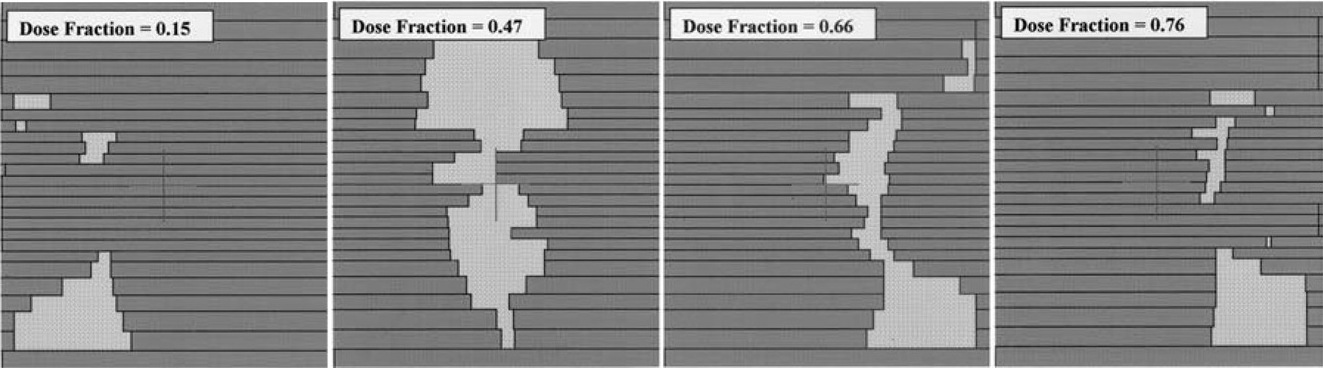
\includegraphics[width=\textwidth]{./cap2/IMRT_Segments_2.jpg}
\caption{Segmenti sagomati con l'MLC per realizzare la modulazione di intensità.}
\label{fig:IMRT_Segments}
\end{figure}

L'MLC oggetto di questa tesi è prodotto dalla Varian Medical Systems (modello Millenium 120). Esso è dotato di due banchi di 60 lamelle che proiettano una dimensione nel piano dell'isocentro di $0.5\,$cm (prime 30 lamelle a partire dal centro) e di $1\,$cm per le rimanenti. In Fig.\ref{fig:MLC_details} sono riportati alcuni dettagli costruttivi.

\begin{figure}
\centering
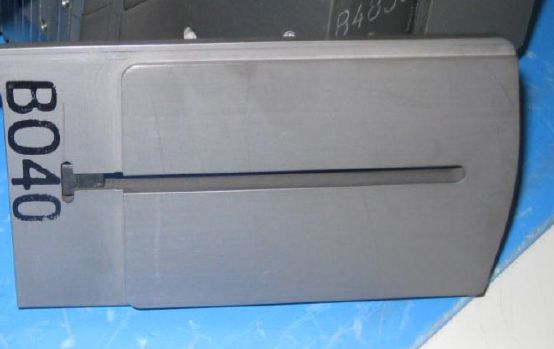
\includegraphics[width=.4\textwidth]{./cap2/MLC_leaf_varian.png}
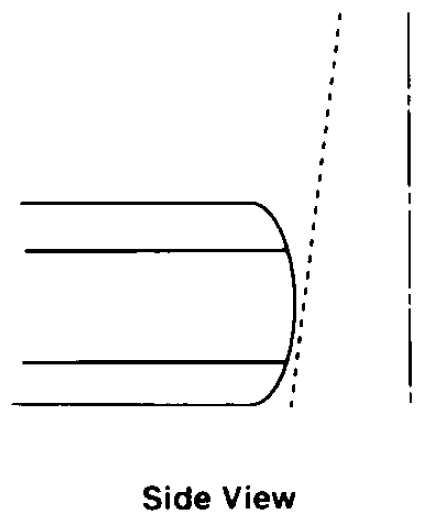
\includegraphics[width=.28\textwidth]{./cap2/MLC_side.png}
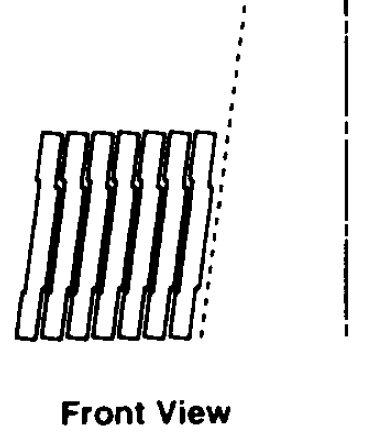
\includegraphics[width=.28\textwidth]{./cap2/MLC_front_2.png}
\caption{Foto e schemi costruttivi dell'MLC Millenium 120.}
\label{fig:MLC_details}
\end{figure}

In particolare i più importanti consistono in:
\begin{description}
\item[\textit{Rounded leaf tip:}] la parte finale del leaf è arrotondata. Questo espediente è adottato per assicurare che i profili di dose collimati dal solo MLC abbiano la stessa penombra per ogni dimensione di campo \cite{Galvin1993a}.
\item[\textit{Tongue and groove:}] il bordo laterale del leaf presenta alternativamente delle sporgenze e rientranze in modo da minimizzare la trasmissione tra un leaf e l'altro (inter-leaf).
\end{description}

Questi dettagli costruttivi comportano degli effetti dosimetrici normalmente trascurabili in 3D-CRT ma che possono diventare rilevanti nelle tecniche ad intensità modulata a causa della sovrapposizione dei vari segmenti.
\begin{figure}[!t]
\centering
a)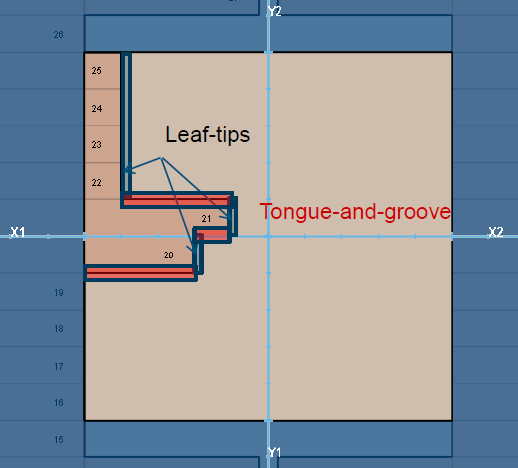
\includegraphics[width=.35\textwidth]{./cap2/MLC_tip-tg.png}
b)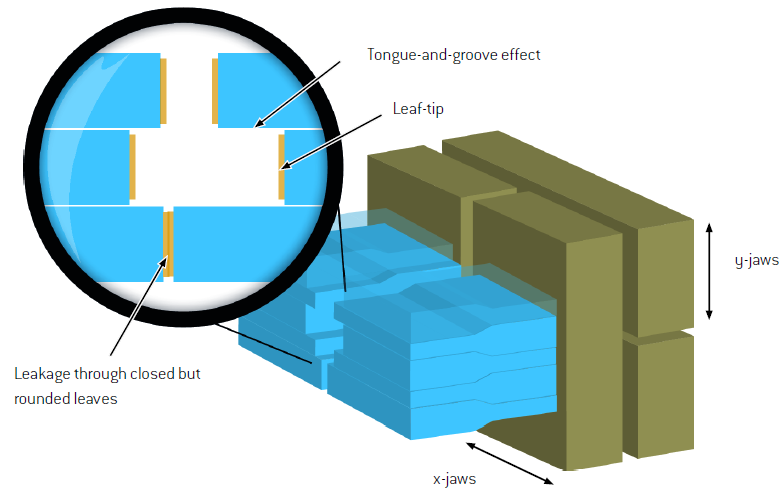
\includegraphics[width=.5\textwidth]{./cap2/MLC_tip-tg_3D.png}
\caption{Sinistra: MLC visto a partire dalla sorgente (\textit{beam's eye view}) con indicate le zone per cui la dose è influenzata dai dettagli costruttivi. Destra: visione 3D dell'MLC con fascio proveniente da destra.}
\label{fig:MLC_Regions}
\end{figure}
In Fig.\ref{fig:MLC_Regions} sono indicate le zone critiche in cui la particolare struttura del leaf (tip e tongue\&{}groove) influenza la distribuzione di dose.\\
I tipici effetti dosimetrici dovuti alla punta arrotondata dei leaf e alla struttura tongue\&{}groove consistono in sovra o sottodosaggi nelle zone di giunzione di campi adiacenti così come mostrato nelle Fig.\ref{fig:MLC_tip_effect} e \ref{fig:MLC_TG_effect}.
\begin{figure}[!t]
\centering
\includegraphics[width=.35\textwidth]{./cap2/tip5.png}
\includegraphics[width=.35\textwidth]{./cap2/tip6.png}\\\vspace{.3cm}
\includegraphics[width=.7\textwidth]{./cap2/MLC_Plots/Abutted/abutted_m.eps}
\caption{La punta arrotondata del leaf comporta un effetto dosimetrico evidente in caso di campi adiacenti come in figura. Nel nostro caso le penombre dei due campi si sommano dando luogo ad un incremento della dose (a \textit{spike}) nella zona di giunzione. I profili di dose mostrati sono acquisiti ad una profondità di $10\,$cm in fantoccio ad acqua con il detector Razor (IBA Dosimetry, vedi Tab.\ref{tab:OF_inter}).}
\label{fig:MLC_tip_effect}
\end{figure}
\begin{figure}
\centering
\includegraphics[width=.35\textwidth]{./cap2/TG1.png}
\includegraphics[width=.35\textwidth]{./cap2/TG2.png}\\\vspace{.3cm}
\includegraphics[width=.7\textwidth]{./cap2/MLC_Plots/TG/TG_Field1-2.eps} \\
\includegraphics[width=.7\textwidth]{./cap2/MLC_Plots/TG/TG_FieldTotm.eps} 
\caption{La somma di campi adiacenti sul bordo laterale del leaf evidenzia dei sottodaggi nelle zone di giunzione dovuti alla struttura tongue\&{}groove. I profili di dose mostrati sono acquisiti ad una profondità di $10\,$cm in fantoccio ad acqua con il detector PFD (IBA Dosimetry, vedi Tab.\ref{tab:OF_inter}).}
\label{fig:MLC_TG_effect}
\end{figure}

La scelta per quanto riguarda le misure effettuate per modellizzare l'MLC è dunque quella di utilizzare delle scansioni che esaltino l'effetto di leaf tip e di tongue\&{}groove come quelle mostrate nelle Fig.\ref{fig:MLC_tip_effect} e \ref{fig:MLC_TG_effect}. Per poter evidenziare in maniera accurata questi effetti di composizione dei campi, è necessario utilizzare dei detector che modifichino il meno possibile le penombre dei profili (i.e. con un volume sensibile minimo).

In particolare sono stati utilizzati i diodi PFD e Razor (IBA Dosimetry) per le seguenti scansioni:\vspace*{.2cm}

\textbf{Effetto di \textit{leaf-tip}:}
\begin{itemize}
\item[-] Profili lungo la direzione di movimento dei leaf (crossline) di campi quadrati collimati dai soli leaf con diodo PFD (IBA Dosimetry), in fantoccio ad acqua e a profondità $10\,$cm. Queste misure permettono di calibrare finemente la posizione dei leaf all'interno del TPS\footnote{Questa operazione è necessaria perché solitamente la posizione nominale dei leaf viene leggermente alterata sulla base di una calibrazione effettuata dalla ditta produttrice per far corrispondere il campo luce con il campo definito dai raggi.}.
\item[-] Profili crossline di campi complementari adiacenti sul lato della punte dei leaf (Fig.\ref{fig:MLC_tip_effect}) con diodo Razor (IBA Dosimetry), in fantoccio ad acqua, a profondità $10\,$cm. Queste misure sono state utilizzate per modellizzare l'effetto da punta arrotondata.
\item[-] Profili di campi complementari come i precedenti, a profondità $1.5\,$cm e $20\,$cm e traslati lateralmente lungo la direzione di movimento dei leaf per verificare la bontà della modellizzazione anche lontano dalle condizioni iniziali.
\end{itemize}

\textbf{Effetto di \textit{tongue\&{}groove:}}
\begin{itemize}
\item[-] Profili di campi complementari adiacenti sul lato del bordo del leaf (Fig.\ref{fig:MLC_tip_effect}), con diodo PFD (IBA Dosimetry), lungo la direzione perpendicolare rispetto al movimento dei leaf (inline), in fantoccio ad acqua e a profondità $10\,$cm. Queste misure sono utilizzate per la modellizzazione dell'effetto di tongue\&{}groove.
\item[-] Profili come i precedenti a profondità $5\,$cm per poter verificare la modellizzazione in condizioni diverse dalla profondità di riferimento.
\end{itemize}




\section{Scelte adottate per la modellizzazione}
Tutte le misure elencate nella sezione precedente, assieme alle misure di dose assoluta (Sez.\ref{sec:dose_ass}), sono state inserite nel modulo del TPS denominato RayPhysics in cui è possibile sviluppare un modello dosimetrico del LINAC. Il processo di modellizzazione consiste nell'ottimizzare una serie di parametri del motore dosimetrico implementato in RayStation (Sez.\ref{sec:algo_Ray}) i quali sono collegati a quantità o fenomeni fisici. Il fine di una modellizzazione è quello di riprodurre le misure sperimentali con un certo grado di accuratezza dipendente dalla tecnica di irradiazione. Nell'ambito di questo lavoro il grado di accuratezza desiderato è quello che viene richiesto per un TPS dedicato alla pianificazione di trattamenti sia in tecnica 3D-CRT (Sez.\ref{sec:accu_3D}) che in tecniche speciali IMRT/VMAT (Sez.\ref{sec:accu_spec}).

I parametri da ottimizzare durante la modellizzazione sono dipendenti l'uno dall'altro in ordine gerarchico. Per questo motivo è necessario seguire un ben determinato schema per evitare di giungere a soluzioni che, pur riproducendo i risultati sperimentali, trovano poco riscontro con la fisica di base. Gli step da seguire per una accurata modellizzazione sono indicati dalla ditta \cite{RaySearchLaboratories2014} e sono stati recentemente discussi anche da Mzenda et al.\cite{Mzenda2014} (vedi Fig.\ref{fig:modeling_steps}).
\begin{figure}
\centering
\includegraphics[width=.8\textwidth]{./cap2/ModelingSteps/ModelingSteps.eps}
\caption{Step da seguire per una accurata modellizzazione \cite{Mzenda2014}.}
\label{fig:modeling_steps}
\end{figure}

\subsection{PDD - Spettro di energia dei fotoni primari}
Il primo step della modellizzazione di un LINAC consiste nell'ottimizzazione dello spettro di energia dei fotoni primari. Questa quantità fisica è una quantità continua e rappresenta la fluenza di fotoni corrispondenti ad una determinata energia in funzione dell'energia stessa. La misura diretta dello spettro di energia in uscita da un LINAC è complessa e richiede strumentazioni normalmente non disponibili nelle aziende ospedaliere. D'altra parte, l'andamento della parte discendente della PDD risulta fortemente legato allo spettro \cite{Khan2010} e questa caratteristica viene impiegata per determinarlo indirettamente.

Il TPS RayStation discretizza uno spettro fotonico di energia $6\,$MV con 10 bin di energia 0.5, 1, 1.5, 2, 2.5, 3, 3.5, 4, 5 e 6 MeV. In RayPhysics sono implementati due tool di ottimizzazione dello spettro fotonico, l'uno detto \textit{parametrico} e l'altro \textit{non-parametrico}. Entrambi questi tool hanno come target massimizzare l'accordo delle PDD calcolate con le PDD misurate nella zona discendente. Il tool parametrico ottimizza delle costanti di fit di una forma funzionale che è implementata in RayPhysics e riproduce analiticamente una serie di spettri clinici \cite{RaySearchLaboratories2014}. Lo spettro continuo ottenuto dalla forma funzionale viene poi integrato e discretizzato nei bin citati precedentemente. Il tool non parametrico d'altra parte, ottimizza direttamente le fluenze con un metodo iterativo.

Il metodo adottato per modellizzare lo spettro fotonico consiste in due step:
\begin{enumerate}
\item Una prima ottimizzazione viene effettuata utilizzando il tool parametrico. Questa scelta permette di partire da uno spettro che riproduce quanto più possibile le PDD (parte discendente) mantenendo però una distribuzione basata su principi fisici.
\item Una volta raggiunto l'accordo migliore ottenibile con il tool parametrico, si è scelto di utilizzare il tool non parametrico effettuando poche iterazioni (da tre ad un massimo di dieci). La ragione di questa scelta sta nel riconoscere che lo spettro analitico, a sua volta discretizzato, può non riprodurre completamente la fenomenologia che da luogo alle curve PDD. Per questo motivo è necessario apportare delle correzioni non-analitiche a patto che non venga perturbata eccessivamente la distribuzione iniziale. Come regola di massima, si è cercato di mantenere i valori dei singoli bin entro il $20-30\%$ del loro valore iniziale.
\end{enumerate}

Lo spettro fotonico ottimizzato secondo la tecnica descritta è riportato in Fig.\ref{fig:Ray_spectr_fot}.
\begin{figure}
\centering
\begin{tabular}{m{.32\textwidth}m{.65\textwidth}}
\vspace*{-0.5cm}\includegraphics[width=.32\textwidth]{./cap2/Ray_spectrum_fot_tab.png} &
\includegraphics[width=.65\textwidth]{./cap2/Ray_spectrum_fot.png}
\end{tabular}
\caption{Spettro fotonico ottimizzato per la modellizzazione della parte discendente delle PDD.}
\label{fig:Ray_spectr_fot}
\end{figure}

\subsection{PDD - Spettro di energia degli elettroni di contaminazione}
La parte ascendente della PDD fino al suo massimo (regione di build-up) è dovuta ai fotoni primari a bassa energia, assieme agli elettroni di contaminazione del fascio (vedi Sez.\ref{sec:dose_electr}). La forma della regione di build-up può essere modulata modificando lo spettro degli elettroni di contaminazione ed i primi bin dello spettro fotonico. In RayPhysics lo spettro di elettroni è dato da una forma funzionale:
\begin{equation}
\psi_{e^-} (E) = A\,E^c\, e^{-E/E_0}
\end{equation}
dove $A$ è un parametro di normalizzazione e $c$ ed $E_0$ sono due parametri da ottimizzare, compresi nell'intervallo $[0,1]$ .

Seguendo le indicazioni della ditta, l'ottimizzazione di questi parametri è stata effettuata con un tool di fit che ottimizza la regione di build-up delle PDD relative al campo più piccolo ($2x2\,$cm$^2$), al campo di riferimento ($10x10\,$cm$^2$) e al campo più grande ($40x40\,$cm$^2$). A seguire, sono stati effettuati degli aggiustamenti manuali in modo da migliorare ulteriormente l'accordo specie per i campi grandi ove la contaminazione elettronica ha un effetto più rilevante. Oltre a ciò, è stato necessario procedere in maniera iterativa modificando manualmente i primi bin dello spettro fotonico e poi ritornando ad ottimizzare lo spettro elettronico fino a raggiungere un accordo accettabile per tutte le dimensioni di campo. Lo spettro elettronico ottimizzato con questa procedura è mostrato in Fig.\ref{fig:Ray_spectrum_ele}.

In Fig.\ref{fig:Ray_PDD_meas_calc} è mostrato qualitativamente l'accordo raggiunto per il calcolo delle PDD a seguito delle ottimizzazioni dello spettro fotonico ed elettronico. La valutazione quantitativa dell'accordo tramite i criteri riportati nella Sez.\ref{sec:accu_spec} sarà discussa in seguito.

\begin{figure}
\centering
\includegraphics[width=\textwidth]{./cap2/Ray_spectrum_ele.pdf}
\caption{Spettro elettronico ottimizzato per la modellizzazione della regione di build-up delle PDD.}
\label{fig:Ray_spectrum_ele}
\end{figure}

\begin{figure}
\centering
\includegraphics[width=\textwidth]{./cap2/Ray_PDD_meas_calc.png}
\caption{Accordo tra PDD misurate e calcolate a seguito delle ottimizzazioni dello spettro fotonico ed elettronico.}
\label{fig:Ray_PDD_meas_calc}
\end{figure}


\subsection{Profili - Off-axis softening, beam profile correction e sorgente di scatter}
Una volta ottimizzato il modello per il calcolo della dose in profondità a centro asse (PDD), si può passare all'ottimizzazione del modello fuori asse (profili). La distribuzione di dose fuori asse è influenzata dalla presenza del flattening-filter (vedi nota a Pag.\pageref{foot:flatt}). Questo dispositivo di forma piramidale attenua la fluenza di fotoni al centro. Ciò provoca anche un aumento dell'energia media del fascio centrale rispetto al fascio fuori asse. Questo processo è noto con il nome di \textit{`off-axis softening'}. RayPhysics modellizza l'off-axis softening introducendo una funzione radiale definita per punti che rappresenta il flattening-filter come un oggetto di acqua equivalente. Lo spessore di acqua equivalente è riscalato in modo che il fascio al centro risulti non attenuato (spessore pari a zero) ed il fascio fuori asse risulti `attenuato' da uno spessore di acqua negativo (vedi Fig.\ref{fig:Ray_flatt}b).
\begin{figure}[!t]
\centering
\begin{tabular}{m{.3\textwidth}m{.6\textwidth}}
\vspace*{-0.5cm}a)\includegraphics[width=.3\textwidth]{./cap2/Ray_flatt1.png} &
\includegraphics[width=.6\textwidth]{./cap2/Ray_flatt2.png}
\end{tabular}
c)\includegraphics[width=.9\textwidth]{./cap2/Ray_flatt3.png}
\caption{Flattening filter: foto e schema costruttivo a). Modellizzazione del flattening filter con la funzione di off-axis softening (b)}
\label{fig:Ray_flatt}
\end{figure}

Accanto alla funzione di off-axis softening, RayPhysics offre un'altra funzione definita per punti con dipendenza radiale detta \textit{beam profile correction}. Questa funzione semplicemente riscala la fluenza primaria con un fattore numerico che dipende dalla distanza radiale dal centro asse. Con la beam profile correction è possibile raffinare la forma del profilo ottimizzando in particolare la zona centrale che usualmente presenta un caratteristico avvallamento dovuto all'attenuazione del flattening filter. \`E inoltre utilizzabile per modellizzare la presenza del collimatore primario il cui effetto si nota agli estremi dei profili diagonali per il campo $40x40\,$cm$^2$\footnote{Il collimatore primario è un materiale ad alta densità che alloggia il target e possiede un'apertura conica in modo da schermare il fascio in tutte le direzioni tranne quella utile clinicamente}.

Si è già parlato nella Sez.\ref{sec:intro} di come la dose fuori asse sia dipendente dai processi di scatter che avvengono all'interno del materiale (\textit{phantom scatter dose}) e dai processi di scatter che avvengono nella testata del LINAC (\textit{head scatter dose}). Mentre i primi sono tenuti in considerazione direttamente dall'algoritmo collapsed-cone-convolution, i secondi vengono tenuti in considerazione in RayPhysics introducendo una sorgente secondaria di fotoni di scatter provenienti dalla base del flattening filter. I parametri per modellizzare la sorgente di scatter consistono in:
\begin{itemize}
\item Dimensione della sorgente di scatter
\item Peso della sorgente di scatter rispetto alla sorgente primaria
\end{itemize}
Modificando questi parametri, si riesce a modulare la parte distale ad alta dose del profilo (spalla) assieme alla parte fuori campo (code).

Per modellizzare accuratamente i profili di dose è necessario ottimizzare simultaneamente le funzioni di off-axis softening e beam profile correction assieme alla sorgente di scatter. L'effetto della sorgente di scatter è dipendente dalla dimensione di campo assumendo più importanza per i campi di dimensioni $> 10x10\,$cm$^2$.\\
Per questo motivo si è scelto di partire con l'ottimizzazione dei profili per il campo di riferimento $10x10\,$cm$^2$ e a seguire dei campi di dimensione superiore con un metodo di iterativo di \textit{trial-and-error}. Durante il processo i parametri sono stati variati entro i range consigliati dalla ditta (mostrati nelle parentesi quadre):
\begin{itemize}
\item Off-axis softening $\in[0,-30]$; risultato: vedi Fig.\ref{fig:Ray_flatt}b.
\item Beam-profile correction $\in[0.95,1.05]$; risultato: vedi Fig.\ref{fig:Ray_beamprof}.
\item Dimensione della sorgente di scatter $\in[1.0,3.5]\,$cm; risultato$\,=2.065\,$cm.
\item Peso della sorgente di scatter $\in[0.05,0.1]$; risultato$\,=0.09048$.
\end{itemize}

\begin{figure}
\centering
\includegraphics[width=.9\textwidth]{./cap2/Ray_beamprof.png}
\caption{Funzione di beam profile correction ottimizzata per modellizzare la forma dei profili dall'asse centrale fino alla parte più periferica schermata dal collimatore primario (modellizzata come un brusco calo della fluenza).}
\label{fig:Ray_beamprof}
\end{figure}

I profili dei campi di dimensione $\leq 4x4\,$cm$^2$ sono stati tenuti in relativa considerazione in questa fase in quanto gli effetti sopra descritti costituiscono fenomeni del secondo ordine rispetto agli effetti collegati alla dimensione della sorgente primaria.

\subsection{Profili - Dimensione della sorgente primaria}
La sorgente primaria di irradiazione è modellizzata in RayStation con un profilo gaussiano ellittico \cite{Chaney1994}. Nel processo di retroproiezione mostrato in Fig.\ref{fig:twosources} si può notare che l'estensione della sorgente riveste grande importanza per i campi piccoli in cui i collimatori parzialmente ne oscurano una porzione. Questo effetto si riflette su una forte influenza delle dimemensioni della sorgente sulle penombre dei campi piccoli.\\
Per questo motivo, la modellizzazione delle dimensioni della sorgente è stata effettuata utilizzando il campo di dimensioni minime ($2x2\,$cm$^2$). In seguito la valutazione è stata estesa anche agli altri campi per aggiustamenti fini del modello.
\begin{figure}
\centering
a)\includegraphics[width=.43\textwidth]{./cap2/Ray_penumbra_wrong.PNG}
b)\includegraphics[width=.43\textwidth]{./cap2/Ray_penumbra_right.PNG}
\caption{(a) una sorgente troppo estesa ($0.1\,$cm) porta ad una sovrastima delle penombre del profilo di dose di dimensioni $2x2\,$cm$^2$ (qui mostrato il profilo \textit{inline} a $10\,$cm di profondità). (b) dimensioni della sorgente ottimizzate ($0.042\,$cm).}
\label{fig:source_2x2}
\end{figure}


I parametri da ottimizzare in questo caso sono le larghezze a mezza altezza del profilo gaussiano ellittico:
\begin{itemize}
\item $x$ width $\in [0.05,0.3]$; risultato: $0.035\,$cm
\item $y$ width $\in [0.05,0.3]$; risultato: $0.042\,$cm
\end{itemize}
In questo caso è stato necessario violare leggermente i limiti suggeriti della ditta (mostrati tra parentesi quadre) per ottimizzare al meglio l'accordo delle penombre (vedi Fig.\ref{fig:source_2x2}).
Coerentemente con le aspettative fisiche, il profilo gaussiano ottimizzato risulta più esteso in direzione $y$ che corrisponde alla direzione di incidenza del fascio elettronico primario.

\subsection{Profili - Calibrazione dei collimatori}
Nelle fasi finali di modellizzazione dei profili è possibile ottimizzare le penombre, specie a campi grandi, utilizzando una funzione di RayPhysics che modifica virtualmente la posizione dei collimatori secondo un'equazione quadratica:
\begin{equation}
pos_{real} = pos_{nominal} - Offset - Gain\cdot pos_{nominal} - Curvature \cdot pos_{nominal}
\label{eq:offset}
\end{equation}
I parametri di \textit{Offset}, \textit{Gain} e \textit{Curvature} sono stati ottimizzati con un tool di fit automatico tenendo in considerazione tutti i profili di dose. I risultati, assieme ai limiti consigliati dalla ditta sono:
\begin{itemize}
\item Collimatori \textit{Y - inline}:
\begin{itemize}
\item \textit{Offset} $\in [0,0.1]$; risultato: $-0.078\,$cm
\item \textit{Gain} $\in [0,0.01]$; risultato: $-0.0008\,$
\item \textit{Curvature} $\in [0,0.001]$; risultato: $0\,$cm$^{-1}$
\end{itemize}
\item Collimatori \textit{X - crossline}:
\begin{itemize}
\item \textit{Offset} $\in [0,0.1]$; risultato: $-0.004\,$cm
\item \textit{Gain} $\in [0,0.01]$; risultato: $-0.0024\,$
\item \textit{Curvature} $\in [0,0.001]$; risultato: $0\,$cm$^{-1}$
\end{itemize}
\end{itemize}

Tutti i parametri sopra citati sono stati ottimizzati utilizzando le curve di dose ottenute per campi collimati con le sole \textit{jaws} (campi \textit{open}). Una volta raggiunto un accordo accettabile per i campi open, è possibile passare alla modellizzazione del MLC utilizzando campi collimati unicamente con quest'ultimo. Questa procedura è utile in quanto permette di ottimizzare i parametri del MLC tenendo fissati gli altri parametri di modello legati unicamente alla sorgenti di fotoni ed elettroni.

\subsection{MLC - Trasmissione}
\label{sec:MLC-trans}
La trasmissione del MLC è modellizzata all'interno di RayPhysics con un unico parametro che tiene conto in media sia della trasmissione interleaf che intraleaf. Si è scelto di misurare questa quantità ponendo una camera a ionizzazione di volume esteso ($0.65\,$cm$^3$) con l'asse perpendicolare alla direzione di movimento dei leaf a $1.5\,$cm di profondità in acqua. I campi utilizzati per questa misura sono riportati nella Fig.\ref{fig:MLC_Trans}. 
\begin{figure}
\centering
a)\includegraphics[width=.43\textwidth]{./cap2/MLC_TransX1.png}
b)\includegraphics[width=.43\textwidth]{./cap2/MLC_TransX2.png}
\caption{Campi utilizzati per la misura di trasmissione del MLC per il banco X1 (a) e il banco X2 (b).}
\label{fig:MLC_Trans}
\end{figure}

La trasmissione è stata calcolata per entrambi i banchi di leaf rispetto alla lettura di dose a campo aperto. La media delle misure per entrambi i banchi è stata inserita come parametro di modello in RayPhysics:
\begin{itemize}
\item Trasmissione $\in [0.01,0.03]$; risultato: $0.01813$.
\end{itemize}
dove nelle parentesi quadre sono indicati i limiti consigliati dalla ditta.


\subsection{MLC - \textit{Offset}}
Per calibrare finemente la posizione dei leaf, RayPhysics implementa la stessa funzione utilizzata per i collimatori (Eq.\ref{eq:offset}). A questo proposito sono state utilizzate scansioni di campi quadrati $2x2$, $3x3$, $4x4$, $5x5$, $10x10$, $15x15$, $20x20$, $30x30\,$cm$^2$ effettuate con il diodo PFD lungo la direzione di movimento dei leaf, a profondità $10\,$cm. Sulla base delle penombre di questi profili si è scelto di ottimizzare il parametro di offset, avendo particolare riguardo per le penombre dei piccoli campi:
\begin{itemize}
\item \textit{Offset} $\in [0,0.1]$; risultato: $0.04\,$cm.
\end{itemize}
In Fig.\ref{fig:MLC_Offset} è riportato il confronto tra profili calcolati e misurati collimati con il solo MLC alla profondità di riferimento $10\,$cm.
\begin{figure}
\centering
\includegraphics[width=\textwidth]{./cap2/MLC_Offset.png}
\caption{Confronto tra profili calcolati e misurati a profondità $10\,$cm collimati con il solo MLC per l'ottimizzazione del parametro di offset.}
\label{fig:MLC_Offset}
\end{figure}

\subsection{MLC - \textit{leaf tip width}}
Le misure descritte nelle Fig.\ref{fig:MLC_tip_effect} sono state impiegate per modellizzare l'effetto dovuto alla punta arrotondata dei leaf. In RayPhysics il parametro da ottimizzare è la \textit{leaf tip width} espressa in centimetri. Questa quantità rappresenta la parte di leaf, a partire dalla punta, proiettata al piano dell'isocentro, per cui la trasmissione viene calcolata come la radice quadrata della trasmissione media del MLC (vedi Fig.\ref{fig:MLC_Regions}).

In Fig.\ref{fig:MLC_tip_model}, è riportato il particolare del confronto dei profili calcolati e misurati per evidenziare l'effetto della punta arrotondata dei leaf. Il parametro di modello è stato variato nel range raccomandato dalla ditta $[0.1, 0.5]\,$cm con step di $0.1\,$cm. Osservando la Fig.\ref{fig:MLC_tip_model} si è scelto come valore di best fit delle misure:
\begin{itemize}
\item \textit{Leaf tip width} $\in [0,0.5]$; risultato: $0.3\,$cm.
\end{itemize}

\begin{figure}[!t]
\centering
\begin{tabular}{m{.38\textwidth}m{.6\textwidth}}
\vspace*{-.3cm}\includegraphics[width=.38\textwidth]{./cap2/MLC_tip_model.png} &
\includegraphics[width=.6\textwidth]{./cap2/MLC_Plots/Abutted/PlotMLC_Tip_modeling.eps}
\end{tabular}
\caption{(a) Modello della punta dei leaf implementato in RayStation. (b) Modellizzazione dell'effetto di leaf tip utilizzando i campi descritti nella Fig.\ref{fig:MLC_tip_effect}.}
\label{fig:MLC_tip_model}
\end{figure}

La modellizzazione dell'effetto di leaf tip è stata in seguito verificata misurando profili di campi adiacenti fuori dall'asse centrale con la stessa tecnica indicata in Fig.\ref{fig:MLC_tip_effect}. I medesimi campi sono stati riprodotti nel TPS utilizzando il parametro di leaf tip width ottimizzato pari a $0.3\,$cm. Il confronto misurato/calcolato è riportato in Fig.\ref{fig:MLC_tip_model_offaxis} e dimostra come il modello della punta del leaf sia accurato anche in situazioni diverse da quelle di riferimento.
\begin{figure}[!t]
\centering
a)\includegraphics[width=.43\textwidth]{./cap2/MLC_Plots/Abutted/PlotMLC_Tip_modeling_offaxis.eps}
b)\includegraphics[width=.43\textwidth]{./cap2/MLC_Plots/Abutted/PlotMLC_Tip_modeling_offaxisSUM.eps}
\caption{(a) profili crossline di campi adiacenti fuori asse centrale misurati con il diodo Razor (IBA Dosimetry) a $10\,$cm di profondità. (b) somma dei campi adiacenti e confronto con il calcolo.}
\label{fig:MLC_tip_model_offaxis}
\end{figure}


\subsection{MLC - \textit{tongue\&{}groove}}
L'effetto di tongue\&{}groove è stato modellizzato utilizzando le misure indicate in Fig.\ref{fig:MLC_TG_effect}. Il parametro che descrive questo effetto in RayPhysics è la \textit{tongue\&{}groove region} espressa in centimetri. Al pari della leaf tip width, la \textit{tongue\&{}groove region} rappresenta la porzione del bordo del leaf, proiettata all'isocentro, per cui la trasmissione viene calcolata come la radice quadrata della trasmissione del MLC (vedi Fig.\ref{fig:MLC_Regions}). 
\begin{figure}[!t]
\centering
\includegraphics[width=.49\textwidth]{./cap2/MLC_Plots/TG/TG_modeling.eps}
\includegraphics[width=.49\textwidth]{./cap2/MLC_Plots/TG/TG_modelingZOOM.eps}
\caption{Modellizzazione dell'effetto di tongue\&{}groove utilizzando i campi descritti nella Fig.\ref{fig:MLC_TG_effect}.}
\label{fig:MLC_TG_modeling}
\end{figure}

Il parametro di \textit{tongue\&{}groove region} è stato variato all'interno dell'intervallo suggerito dalla ditta ed i risultati sono presentati nella Fig.\ref{fig:MLC_TG_modeling}. Sulla base di questi risultati, il parametro di best fit scelto è:
\begin{itemize}
\item \textit{Tongue\&{}groove region} $\in [0, 0.1]$; risultato: $0.05\,$cm
\end{itemize}
Questo risultato è stato poi testato ripetendo la stessa procedura ad una diversa profondità ($5\,$cm) ottenendo i medesimi risultati.\\


\section{Analisi quantitativa dell'accordo calcolato/misurato}
I confronti calcolato/misurato sono presentati nelle sezioni precedenti unicamente a livello qualitativo. Per la validazione rigorosa del calcolo di un TPS c'è bisogno di un criterio quantitativo come discusso nella Sez.\ref{sec:accu_spec}. 

Allo stato attuale di sviluppo (versione 4.7), RayPhysics permette di esportare in formato ASCII le curve calcolate. Tuttavia non offre un tool di valutazione quantitativo dell'accordo tra il misurato ed il calcolato. Per questo motivo è stato sviluppato \textit{in-house} un programma in linguaggio MATLAB capace di analizzare le curve secondo i criteri suggeriti dal protocollo ESTRO \cite{Mijnheer2004} (Tab.\ref{tab:tol}) aggiornato per le tecniche speciali secondo le indicazioni AAPM \cite{Ezzell2009}. Un esempio di confronto quantitativo di una PDD calcolata e misurata è stato già riportato in Fig.\ref{fig:Ray_PDD_meas_calc}.

L'analisi è stata ripetuta per tutte le PDD e i profili utilizzati per la modellizzazione. In Tab.\ref{tab:Ray_ALL_meas_calc} sono riportati i valori del livello di confidenza dell'indice $\gamma$ per PDD e profili corrispondenti alle varie dimensioni di campo. Il calcolo è stato effettuato adottando le seguenti tolleranze (sulla base delle indicazioni riportate in Tab.\ref{tab:tol}):
\begin{itemize}
\item PDD: differenza di dose $\leq 2\%$; distanza di accordo $\leq 2\,$mm
\item Profili: differenza di dose $\leq 3\%$; distanza di accordo $\leq 2\,$mm
\end{itemize}

\begin{table}
\centering
\arrstr{1.2}

\begin{tabular}{lcc}
\toprule
Tipo & Campo (cm$^2$) & $CL(\gamma)$\\
\midrule
PDD & $2x2$ & 0.53\\
PDD & $3x3$ & 0.39\\
PDD & $4x4$ & 0.48\\
PDD & $5x5$ & 0.51\\
PDD & $7x7$ & 0.53\\
PDD & $10x10$ & 0.38\\
PDD & $15x15$ & 0.45\\
PDD & $20x20$ & 0.67\\
PDD & $30x30$ & 0.69\\
PDD & $40x40$ & 0.82\\
\bottomrule
\end{tabular}
\vspace*{.2cm}
\begin{tabular}{lcc}
\toprule
Tipo & Campo (cm$^2$) & $CL(\gamma)$\\
\midrule
Prof. Inline & $2x2$ & 0.23\\
Prof. Inline & $3x3$ & 0.31\\
Prof. Inline & $4x4$ & 0.32\\
Prof. Inline & $5x5$ & 0.43\\
Prof. Inline & $7x7$ & 0.43\\
Prof. Inline & $10x10$ & 0.49\\
Prof. Inline & $15x15$ & 0.53\\
Prof. Inline & $20x20$ & 0.58\\
Prof. Inline & $30x30$ & 0.76\\
Prof. Inline & $40x40$ & 0.97\\
\bottomrule
\end{tabular}
\vspace*{.2cm}
\begin{tabular}{lcc}
\toprule
Tipo & Campo (cm$^2$) & $CL(\gamma)$\\
\midrule
Prof. Crossline & $2x2$ & 0.30\\
Prof. Crossline & $3x3$ & 0.30\\
Prof. Crossline & $4x4$ & 0.34\\
Prof. Crossline & $5x5$ & 0.37\\
Prof. Crossline & $7x7$ & 0.36\\
Prof. Crossline & $10x10$ & 0.37\\
Prof. Crossline & $15x15$ & 0.44\\
Prof. Crossline & $20x20$ & 0.53\\
Prof. Crossline & $30x30$ & 0.68\\
Prof. Crossline & $40x40$ & 0.68\\
\bottomrule
\end{tabular}
\begin{tabular}{lcc}
\toprule
Tipo & Campo (cm$^2$) & $CL(\gamma)$\\
\midrule
Prof. MLC & $2x2$ & 0.46\\
Prof. MLC & $3x3$ & 0.46\\
Prof. MLC & $4x4$ & 0.34\\
Prof. MLC & $5x5$ & 0.50\\
Prof. MLC & $10x10$ & 0.44\\
Prof. MLC & $15x15$ & 0.58\\
Prof. MLC & $20x20$ & 0.68\\
Prof. MLC & $30x30$ & 0.90\\
\bottomrule
\end{tabular}
\caption{Analisi quantitativa dell'accordo tra PDD e profili calcolati/misurati utilizzando il criterio del livello di confidenza dell'indice $\gamma$ \cite{Mijnheer2004,Ezzell2009}. L'analisi è applicata alle curve di dose ottenute definendo il campo unicamente con i collimatori \textit{jaws} (PDD, Prof.Inline, Prof.Crossline) oppure con il solo MLC (Prof. MLC).}
\label{tab:Ray_ALL_meas_calc}
\end{table}

I livelli di confidenza (CL) calcolati risultano tutti inferiori a 1 che rappresenta il criterio di accettazione. Si può notare un trend di peggioramento dei valori di CL all'aumentare delle dimensioni del campo di irradiazione. Ciò è dovuto principalmente alle scelte effettuate durante la modellizzazione di privilegiare i campi di piccole dimensioni in quanto più rilevanti per le tecniche di irradiazione speciali IMRT e VMAT.





\section{Test clinici e risultati}
Osservando le Tab.\ref{tab:Ray_ALL_meas_calc}, è possibile affermare che il TPS riesce a riprodurre le misure effettuate per il suo commissioning con il grado di accuratezza necessario alla pianificazione di trattamenti in tecniche 3D-CRT e speciali IMRT/VMAT. Tuttavia,  sia i documenti AAPM \cite{Ezzell2009} che ESTRO \cite{Mijnheer2005} raccomandano un'ulteriore step di validazione, in particolar modo per le tecniche speciali.\\
A questo proposito si è scelto di effettuare una prima validazione del modello utilizzando i fantocci virtuali messi a disposizione dall'AAPM TG119 \cite{Ezzell2009} (vedi Fig.\ref{fig:TG119_phantoms}). A seguire è stata effettuata la validazione per casi clinici reali, pianificati in tecnica volumetrica ad intensità modulatata (VMAT).

La tecnica utilizzata per la validazione dei casi del TG119 e di quelli clinici prende il nome di \textit{verifica pre-trattamento} che verrà presentata nella sezione successiva.

\subsection{La verifica pre-trattamento}
La verifica pre-trattamento è stata introdotta con l'avvento delle tecniche speciali come parte del processo di assicurazione di qualità del trattamento radioterapico. In particolare, le correnti guide ESTRO \cite{Mijnheer2005} raccomandano di effettuare una verifica \textit{patient-oriented} per ogni trattamento speciale che si vuole mettere in atto sul paziente. Viene inoltre affermato che la verifica pre-trattamento costituisce uno strumento efficace per la validazione della modellizzazione di un TPS dedicato alla pianificazione di tecniche ad intensità modulata.

In breve, la verifica pre-trattamento consiste nell'erogare il piano di trattamento radioterapico su un sistema in grado di effettuare una misurazione della distribuzione di dose\footnote{Solitamente viene misurato un sottoinsieme dell'intera distribuzione (es. punti, piani singoli, piani multipli, spirali\ldots)}. Questa misura viene poi confrontata con la distribuzione di dose predetta dal TPS.

Il confronto delle due distribuzioni di dose si effettua con il medesimo criterio del $\gamma$\textit{-index} presentato nell'Eq.\ref{eq:gamma} a pag.\pageref{eq:gamma}. Questo criterio può essere esteso al caso bidimensionale o volumetrico e applicato a seconda della distribuzione di dose che il sistema di verifica è in grado di misurare (planare, multi-planare o volumetrica) \cite{Low2011}. I valori del $\gamma$\textit{-index} per ogni punto di misura costituiscono una distribuzione statistica che può essere presentata in forma di istogramma (Fig.\ref{fig:gamma_histo}).
\begin{figure}
\centering
\includegraphics[width=\textwidth]{./cap2/gamma_histo.png}
\caption{Esempio di distribuzione del $\gamma$\textit{-index} per un confronto tra una distribuzione di dose misurata e una calcolata.}
\label{fig:gamma_histo}
\end{figure}

Un piano clinico può essere accettato se la percentuale di punti dell'istogramma per cui $\gamma-index > 1$ è minore del 10\%. In altre parole si accetta un piano di trattamento se il \textit{passing-rate} del $\gamma$\textit{-index} risulta maggiore del 90\%. Le tolleranze consigliate per la valutazione del $\gamma$\textit{-index} nel caso di piani IMRT/VMAT sono rispettivamente $3\%$ della dose massima e $3\,$mm di distanza di accordo \cite{Ezzell2009}.

Il sistema di verifica pre-trattamento disponibile presso l'azienda ospedaliera di Teramo è denominato MatriXX ed è commercializzato dalla IBA Dosimetry (Schwarzenbruck, Germany). Questo sistema è costituito da una matrice di 1024 rivelatori a camera a ionizzazione disposti su un piano e permette quindi una misurazione planare della dose. Per simulare le condizioni di irraggiamento del paziente, il MatriXX viene posto all'interno di un fantoccio cubico denominato MultiCube (vedi Fig.\ref{fig:MatriXX}). 
\begin{figure}
\centering
a)\includegraphics[width=.43\textwidth]{./cap2/MatriXX_Alone.png}
b)\includegraphics[width=.43\textwidth]{./cap2/MatriXX_Cube.png}
\caption{Rivelatore MatriXX (a) e suo posizionamento all'interno del MultiCube (b) sul lettino del LINAC per effettuare la verifica pre-trattamento}
\label{fig:MatriXX}
\end{figure}
Questo fantoccio è costituito da un materiale che per densità e purezza si comporta similmente all'acqua quando irraggiato da un fascio clinico\footnote{Materiale comunemente noto in gergo come \textit{acqua-equivalente}.}. 

Il processo di verifica pre-trattamento si realizza con questa strumentazione effettuando uno studio di tomografia computerizzata (CT) del complesso MatriXX più MultiCube. Su questa CT viene ricalcolato il piano di trattamento da verificare da cui viene estratto il piano di dose predetto a livello dei detector (vedi Fig.\ref{fig:MatriXX_CT}).
\begin{figure}
\centering
a)\includegraphics[width=.43\textwidth]{./cap2/MatriXX_CT.png}
b)\includegraphics[width=.43\textwidth]{./cap2/MatriXX_CT_Plan.png}
\caption{(a) studio CT del complesso MatriXX più MultiCube. (b) erogazione di un piano di trattamento volumetrico ad arco sul complesso MatriXX più MultiCube per la verifica pre-trattamento.}
\label{fig:MatriXX_CT}
\end{figure}
\begin{figure}
\centering
\includegraphics[width=\textwidth]{./cap2/gamma_comparison.png}
\caption{Confronto tra piano di dose misurato (a) e calcolato (b) in termini di profili (c) o di mappa del $\gamma$\textit{-index} (d).}
\label{fig:gamma_comparison}
\end{figure}

Avendo a disposizione il piano di dose calcolato e misurato, il software OmniPro ImRT+ v.2.0 (IBA Dosimetry) fornisce i risultati del confronto in termini di $\gamma$\textit{-index} sotto forma di mappa (vedi Fig.\ref{fig:gamma_comparison}) e sotto forma di istogramma (Fig.\ref{fig:gamma_histo}) su cui è possibile applicare i criteri di accettazione.

\subsection{Verifica della modellizzazione per tecniche IMRT e VMAT con i test dell'AAPM TG-119}
\begin{figure}
\centering
\includegraphics[width=.8\textwidth]{./cap2/TG119_phantoms}
\caption{Fantocci virtuali proposti dall'AAPM TG-119 \cite{Ezzell2009} per la validazione del calcolo da TPS per tecniche speciali IMRT/VMAT.}
\label{fig:TG119_phantoms}
\end{figure}

Il task-group 119 (TG-119) della AAPM \cite{Ezzell2009} propone una serie di test e tolleranze da rispettare per poter procedere all'implementazione clinica della tecnica IMRT \textit{step and shoot} (SMLC) o \textit{dinamica} (DMLC) (Sez.\ref{sec:accu_spec}). Tuttavia è stato dimostrato come questi test possano essere considerati validi anche per l'implementazione della tecnica VMAT \cite{Mynampati2012}.

Il TG-119 richiede di pianificare dei trattamenti su fantocci virtuali rispettando dei determinati vincoli dosimetrici e di procedere poi alla verifica pre-trattamento. Lo strumento di valutazione della verifica è il $\gamma$\textit{-index} con tolleranze pari al 3\% della dose massima e $3\,$mm di distanza di accordo. Il criterio di accettabilità è che il pass-rate del $\gamma$\textit{-index} sia maggiore del 90\%.

Si è scelto di applicare la serie di test del task group a tutte le tecniche ad intensità modulata disponbili (IMRT-SMLC, IMRT-DMLC e VMAT). In Fig.\ref{fig:TG119_stats} sono riportati in forma schematica i vincoli dosimetrici imposti dal task group e il valore raggiunto con il TPS RayStation. In tutti i casi i vincoli dosimetrici sono risultati compatibili o migliori di quelli raggiunti dal TG-119.
\begin{figure}
\centering
a)\includegraphics[width=.7\textwidth]{./cap2/TG119_Plots/Target_Coverage.eps}\\
\centerline{
b)\includegraphics[width=.55\textwidth]{./cap2/TG119_Plots/Target_Hotspots.eps}
\includegraphics[width=.7\textwidth]{./cap2/TG119_Plots/OARs.eps}}
\caption{Vincoli dosimetrici suggeriti (Goal) e raggiunti (TG119) dal task group 119 confrontati con i valori raggiunti con il TPS RayStation per le tecniche SMLC, DMLC e VMAT. (a) confronto dei vincoli per la copertura dei target (valori al di sopra del Goal sono vantaggiosi). (b) confronto dei vincoli per gli hotspot nei target e negli organi a rischio (valori al di sotto del Goal sono vantaggiosi). }
\label{fig:TG119_stats}
\end{figure}

I risultati della verifica pre-trattamento effettuata applicando le direttive del TG-119 sono riportati nella Fig.\ref{fig:TG_119_gamma}.
\begin{figure}
\centering
\includegraphics[width=\textwidth]{./cap2/TG119_Plots/TG_119_gamma.eps}
\caption{Confronto dei pass-rate del $\gamma$\textit{-index} tra il TG-119 ed i piani SMLC, DMLC e VMAT prodotti con il TPS RayStation. I valori del TG-119 sono rappresentati con barre di errore che costituiscono il massimo ed il minimo pass-rate registrato dal task group.}
\label{fig:TG_119_gamma}
\end{figure}
Si può notare che in tutti i casi i pass-rate ottenuti a livello locale risultano superiori o compresi all'interno degli intervalli di variabilità registrati dal TG-119. Questa rappresenta la validazione pre-clinica della modellizzazione del TPS.

\subsection{Verifica della modellizzazione per casi clinici}
Evidenze scientifiche posteriori all'emissione del report TG-119 hanno dimostrato che, in alcuni casi, le tolleranze proposte dal task group pari al 3\% della dose massima e $3\,$mm in distanza di accordo possano essere poco sensibili ad errori rilevanti dal punto di vista clinico. Ad esempio, nel lavoro del 2013 di Heilemann et al.\cite{Heilemann2013} vengono simulati per la tecnica VMAT alcuni errori di posizionamento del multi-leaf-collimator che determinano un cambiamento significativo della distribuzione di dose al target. Una verifica pre-trattamento di tali piani modificati utilizzando delle tolleranze sul $\gamma$\textit{-index} pari a 3\%,$3,$mm fornisce un valore accettabile (i.e. pass-rate$> 90\%$). A seguito della disamina del problema, gli autori concludono che un criterio di confronto calcolato/misurato più appropriato per garantire la qualità dei trattamenti VMAT è la valutazione del $\gamma$\textit{-index} con tolleranze pari al $2\%$ della dose massima e $2\,$mm di distanza di accordo. Per questo motivo, in fase di immissione nella routine clinica della tecnica di trattamento VMAT, sono state effettuate ulteriori verifiche della modellizzazione su casi di pazienti reali. In particolare sono stati reclutati 5 pazienti con target di tipo prostata e 5 pazienti con target di tipo testa/collo. Su questi pazienti sono stati pianificati dei trattamenti clinici in tecnica VMAT e sottoposti in seguito a verifica pre-trattamento adottando le tolleranze $3\%,3\,mm$ e $2\%,2\,mm$. Con la tolleranza $2\%,2\,mm$ è stato rieffettuato il computo dell'indice $\gamma$ per i piani test proposti del TG-119.

\begin{table}
\centering
\arrstr{1.2}
\centerline{
\begin{tabular}{lll}
\toprule
VMAT clin. & $\gamma(3\%,3\,mm)$ & $\gamma(2\%,2\,mm)$ \\
\midrule
Pr1  & 98.1\% & 96.2\% \\
Pr2  & 98.9\% & 96.9\% \\
Pr3  & 97.8\% & 94.2\% \\
Pr4  & 99.7\% & 96.9\% \\
Pr5  & 100\%  & 100\% \\
\bottomrule
\end{tabular}
\begin{tabular}{lll}
\toprule
VMAT clin. & $\gamma(3\%,3\,mm)$ & $\gamma(2\%,2\,mm)$ \\
\midrule
HN1  & 100\%  & 98.6\% \\
HN2  & 99.9\% & 96.6\% \\
HN3  & 100\%  & 98.2\% \\
HN4  & 98.8\% & 93.6\% \\
HN5  & 99.6\% & 94.3\%\\
\bottomrule
\end{tabular}
}
\vspace*{.3cm}
\begin{tabular}{lll}
\toprule
TG119 & $\gamma(3\%,3\,mm)$ & $\gamma(2\%,2\,mm)$ \\
\midrule
I1-Multitarget  & 99.6\% & 98.7\% \\
I2-Prostate     & 100\% & 98.0\% \\
I3-HN           & 98.9\% & 95.6\% \\
I4-C-shape Easy & 100\% & 97.0\% \\
I5-C-shape Hard & 97.2\%  & 94.8\%  \\
\bottomrule
\end{tabular}
\caption{Valori dei pass-rate del $\gamma$\textit{-index} con tolleranze $3\%,3\,mm$ e $2\%,2\,mm$ relativi a verifiche pre-trattamento di piani VMAT su pazienti reali di tipo prostata (Pr.) e testa/collo (HN) assieme ai test del TG-119.}
\label{tab:TG119_gamma_strict}
\end{table}

Nella Tab.\ref{tab:TG119_gamma_strict} è mostrato il confronto tra i pass-rate ottenuti al variare della tolleranza. Nonostante si noti un abbassamento generale dei valori, il criterio del pass-rate$>90\%$ resta comunque soddisfatto sia per tolleranze pari a $3\%,3\,mm$ che $2\%,2\,mm$. Questi test rappresentano la validazione finale della modellizzazione del TPS RayStation. A seguito di questi risultati, il TPS è stato posto in utilizzo clinico nella pianificazione dei trattamenti radioterapici in tecniche 3D-CRT, IMRT-SMLC, IMRT-DMLC e VMAT presso la U.O.C. di Radioterapia della ASL di Teramo.










\chapter{La radioterapia adattiva. Implementazione iniziale e sviluppi futuri}
\minitoc
\textsf{}

\section{Origini e razionale della radioterapia adattiva}
Per radioterapia adattiva o \textit{adaptive radiation therapy} si intende una tecnica di erogazione della dose che si `adatta' ai possibili cambiamenti che si verificano durante il trattamento, rispetto alla situazione iniziale di pianificazione. I cambiamenti che si possono verificare durante un trattamento radiante possono essere di varia natura e riguardare sia l'interno del paziente (progressione/regressione del target, dimagrimento, diverso stato di riempimento degli organi cavi), sia il suo  posizionamento sul lettino di trattamento (incertezza di setup). 

Il metodo tradizionale di affrontare il problema dei cambiamenti rispetto alla situazione di pianificazione è esposto nei report della \textit{International Commission of Radiological Units} (ICRU) no.50 e no.62, ripreso anche nel recente report no.83 per le tecniche ad intensità modulata \cite{ICRU2010}. Esso consiste nell'espandere i target di un certo margine di sicurezza in modo da assicurare la loro corretta irradiazione anche in presenza delle succitate incertezze.
\begin{figure}
\centering
a)\includegraphics[width=.25\textwidth]{./cap3/ptv.png}
b) \includegraphics[width=.64\textwidth]{./cap3/adapt0.png}
\caption{(a) definizioni ICRU dei volumi coinvolti nella pianificazione del trattamento radioterapico. (b) Processo standard di pianificazione ed erogazione del piano del trattamento.}
\label{fig:adapt0}
\end{figure}

Nella Fig.\ref{fig:adapt0} sono riportate le definizioni dei volumi coinvolti nella pianificazione del trattamento radioterapico assieme ad uno schema del processo standard di pianificazione ed erogazione del piano del trattamento.\\
Il meccanismo che ha portato alla definizione dei singoli volumi procede in vari step:
\begin{description}
\item[Gross Target Volume (GTV):] questo volume identifica il tumore a livello macroscopico (rivelabile attraverso strumenti ottici, imaging radiologico, esame obiettivo clinico,\ldots).

\item[Clinical Target Volume (CTV):] volume che comprende il GTV ed un margine attorno ad esso in cui vi è alta probabilità di presenza di malattia che ancora non si manifesta clinicamente (sub-clinica).

\item[Internal Target Volume (ITV):] volume che aggiunge al CTV un margine (detto \textit{internal margin o IM}) che serve a comprendere il possibile movimento del target per cause interne al paziente (e.g. respiro, stato di riempimento degli organi adiacenti, battito cardiaco\ldots).

\item[Planning Target Volume (PTV):] volume che aggiunge all'ITV un margine per comprendere l'incertezza dovuta al posizionamento del paziente rispetto alla posizione di pianificazione (\textit{setup margin o SM}).

\item[Treated Volume:] volume che riceve una dose maggiore del 98\% della dose di prescrizione.

\end{description}

Il metodo per calcolare i margini necessari alla definizione del PTV si basa su uno studio statistico in cui si effettua un analisi dei possibili errori di posizionamento del target rispetto alla posizione pianificata, distinguendoli in errori sistematici ed errori random. Una delle formule più note è dovuta a Marcel Van Herk \cite{ICRU62}:
\begin{equation}
PTV_{margin} = 2.5\Sigma + 0.7\sigma
\end{equation}
dove $\Sigma$ rappresenta l'errore sistematico ossia quell'errore che si ripete per tutto il ciclo di trattamento (es. paziente dimagrito rispetto alla pianficazione) mentre $\sigma$ è l'errore random (es. movimento d'organo).

In un approccio non adattivo i margini da dare al CTV per arrivare al PTV si trovano effettuando uno studio di coorte per un fissato sito di irradiazione. In questo studio si valutano gli errori sistematici e random su una popolazione di pazienti e si applica la formula di Van Herk secondo le direttive ICRU \cite{ICRU62}. La pianificazione viene quindi effettuata stabilendo delle condizioni di irradiazione del planning target volume (PTV)  che vengono ripetute per tutto il ciclo di trattamento (Fig.\ref{fig:adapt0}b).\\
Questo tipo di approccio può tuttavia non essere ottimale per lo specifico paziente come indicato schematicamente nella Fig.\ref{fig:margins}. In un approccio di \textit{adaptive radiotherapy} è invece possibile studiare il singolo caso ed adattare il trattamento allo specifico paziente.
\begin{figure}
\centering
\includegraphics[width=.8\textwidth]{./cap3/margins.png}
\caption{La formula di Van Herk per ottenere il PTV utilizzando uno studio di coorte (a) da luogo a margini che possono essere sovrabbondanti per il singolo paziente (b).}
\label{fig:margins}
\end{figure}

Il termine \textit{adaptive radiotherapy} è stato introdotto per la prima volta  da Yan et al.\cite{Yan1996}. In questo lavoro veniva per la prima volta proposto un adattamento del piano di cura a seguito di rilevazioni effettuate nelle prime cinque sedute di trattamento con un dispositivo in grado di `fotografare' la posizione del paziente e di confrontarla rispetto alla posizione di pianificazione. Il dispositivo in oggetto è denominato \textit{portal imager} e consiste in un pannello elettronico montato sul LINAC che è in grado di generare un'immagine utilizzando raggi di energia dell'ordine dei MeV allo stesso modo in cui vengono generate le radiografie classiche con i raggi di energia dell'ordine del keV. A seguito di queste rilevazioni Yan proponeva di stimare l'errore sistematico paziente-specifico calcolando la media delle deviazioni tra posizione pianificata e posizione di trattamento rilevate nelle prime cinque sedute e di adattare il piano spostando il centro di irradiazione di questa quantità.

\begin{figure}[!t]
\centering
a)\includegraphics[width=.95\textwidth]{./cap3/adapt1.png}
b)\includegraphics[width=.95\textwidth]{./cap3/adapt2.png}
\caption{(a) approccio di adaptive radiotherapy in cui viene unicamente modificato l'isocentro del piano a seguito di rilevazioni dell'errore di posizionamento del paziente tramite portal-imager (PI). (b) approccio di adaptive radiotherapy in cui alla modificazione dell'isocentro si aggiunge la modificazione dei margini attorno al CTV in base a rilevazioni di tomografia computerizzata (CT); in questo caso il piano di trattamento si adatta al nuovo PTV \textit{confidence-limit PTV o cl-PTV} stimato dopo le cinque sedute di controllo.}
\label{fig:adaptYAN}
\end{figure}

Pochi anni dopo sempre Yan et al.\cite{Yan2000} pubblicano un altro studio in cui aggiungono alla rilevazione tramite portal-imager anche un rilevazione di tomografia computerizzata del paziente per le prime cinque sedute in modo da osservare il problema del movimento d'organo oltre all'errore di setup. Questo permise agli autori di definire un PTV paziente-specifico che veniva calcolato con la procedura seguente:
\begin{itemize}
\item Si delinea il CTV sui cinque studi CT acquisite in sede delle prime cinque frazioni di trattamento.
\item Si uniscono i contorni dei cinque CTV con il CTV di pianficazione a costituire il cosiddetto \textit{CTV-hull}.
\item Si espande il \textit{CTV-hull} del margine corrispondente all'errore sistematico misurato tramite le cinque rilevazioni tramite portal-imager per formare il \textit{confidence-limit PTV o cl-PTV}. 
\end{itemize}
Entrambi gli approcci adaptive presentati in questa sezione sono raffigurati schematicamente nella Fig.\ref{fig:adaptYAN}.

\`E stato dimostrato che la riduzione del PTV e la conseguente ripianficazione possibile grazie all'applicazione di queste tecniche di adaptive radiotherapy ha portato ad un decremento significativo delle tossicità per gli organi sani, preservando il controllo della malattia \cite{Park2012}. Questo dato è facilmente comprensibile con il paradigma dell'arancia di Verellen \cite{Verellen2007} illustrato in Fig.\ref{fig:verellen}. In pratica, il volume occupato dalla buccia di un'arancia è comparabile con il volume dell'arancia stessa. Tradotto, la riduzione anche di pochi millimetri del PTV può comportare una riduzione del volume da irradiare considerevole che porta ad un maggior risparmio dei tessuti sani.
\begin{figure}[!t]
\centering
\includegraphics[width=.6\textwidth]{./cap3/Verellen.png}
\caption{Il paradigma dell'arancia di Verellen \cite{Verellen2007} per illustrare l'importanza della riduzione dei margini in radioterapia.}
\label{fig:verellen}
\end{figure}



\section{Il concetto attuale di \textit{adaptive-radiotherapy} implementato in RayStation}
Il concetto di radioterapia adattiva ha subito negli anni vari aggiornamenti e revisioni ma solo negli ultimi anni è divenuto oggetto di grande interesse. Ciò è dovuto principalmente all'avvento  delle tecniche di imaging per il controllo volumetrico del posizionamento del paziente installate sui moderni LINAC. La tecnica più diffusa implementata nei moderni LINAC è denominata \textit{cone-beam-computed-tomography o CBCT}. Essa consiste in un sistema capace di ricostruire immagini tomografiche del paziente utilizzando un fascio conico di raggi X e di confrontarle con lo studio CT di pianificazione.

\begin{figure}[!t]
\centering
\centerline{
\includegraphics[width=1.2\textwidth]{./cap3/HN_DVH.png}}
\caption{(a) scansione CT del distretto testa-collo di un paziente con delineato in rosso il target e negli altri colori gli organi a rischio. (b) scansione CBCT di controllo a 2.5 settimane con evidente riduzione di volume del target. (c-d) confronto delle distribuzioni di dose di pianificazione (linea continua) e di valutazione (linea tratteggiata). L'istogramma (d) è detto \textit{istogramma dose-volume o DVH} e rappresenta quantitativamente come la distribuzione di dose copre i volumi delineati nello studio CT. \`E da notare come il cambiamento del paziente comporti una variazione della distribuzione di dose agli organi e al target.}
\label{fig:HN_DVH}
\end{figure}

 Nella Fig.\ref{fig:HN_DVH} è illustrato un tipico esempio di irradiazione del distretto testa-collo di largo interesse per la radioterapia adattiva per i grossi cambiamenti che avvengono in itinere nell'anatomia del paziente. A causa dei rapidi gradienti di dose realizzati con le tecniche ad intensità modulata, piccoli cambiamenti di anatomia del paziente possono avere un largo impatto sulla distribuzione di dose finale sia per il target che per gli organi a rischio (Fig.\ref{fig:HN_DVH}d). \\
 
Il TPS RayStation affronta il problema della radioterapia adattiva offrendo una soluzione `all-in-one' che si articola in cinque principali step:
\begin{itemize}
\item[\textbf{a)}] \textbf{Acquisizione degli studi CBCT:} le CBCT acquisite dal sistema di imaging montato sul LINAC vengono spedite al TPS.
\item[\textbf{b)}] \textbf{Deformazione elastica:} viene effettuata una registrazione elastica tra la CT di pianificazione e le CBCT. Questa operazione consiste nel trovare il campo di deformazione geometrico che, se applicato alla CBCT di controllo,   trasforma quest'ultima nella CT di pianificazione. La trasformazione in oggetto è unicamente geometrica: vengono solo variate le coordinate dei pixel ma non il loro valore in scala di grigi.
\item[\textbf{c)}] \textbf{Calcolo della dose in CBCT:} il piano di trattamento viene trasferito alle CBCT e ricalcolato in modo da ottenere la distribuzione di dose relativa alle specifiche frazioni. 
\item[\textbf{d)}] \textbf{Deformazione delle dosi:} sulla base della registrazione deformabile geometrica viene deformata la distribuzione di dose calcolata in CBCT e riportata sulla CT di pianificazione. In questo modo si possono confrontare le distribuzioni di dose pianificata ed effettivamente erogata sulla CT di pianificazione.
\item[\textbf{e)}] \textbf{Adattamento del piano:} sulla base delle differenze tra le distribuzioni di dose pianificata ed erogata si decide o meno di effettuare una ripianificazione del trattamento.
\end{itemize}

Tutti questi passaggi (a parte il primo) presentano delle criticità che al giorno d'oggi non sono del tutto superate in maniera condivisa. In particolare, le questioni su cui vi è ancora un largo dibattito nella comunità scientifica possono essere riassunte nei punti seguenti:\\

\noindent\textbf{Deformazione elastica:}
\begin{itemize}
\item Quale accuratezza è raggiungibile?
\item Quale è il miglior modo di effettuare le deformazioni?
\end{itemize}
\textbf{Calcolo della dose in CBCT}
\begin{itemize}
\item Quanto è accurato il calcolo della dose in CBCT?
\end{itemize}
\textbf{Deformazione delle dosi:}
\begin{itemize}
\item Quanto è giusto deformare le dosi utilizzando la trasformazione geometrica?
\end{itemize}
\textbf{Adattamento del piano:}
\begin{itemize}
\item Sulla base di quale metrica si può decidere la ripianificazione?
\item Qual è il momento migliore per la ripianificazione?
\item Che livello di verifica pre-trattamento è richiesto per il piano adattato?
\end{itemize}

Come mostrato in un recente point/counterpoint pubblicato su \textit{Medical Physics} \cite{Schultheiss2012}, la comunità scientifica non è ancora giunta ad una risposta precisa ed esaustiva per le domande sopra elencate. Per questo motivo il commissioning del TPS dal punto di vista della radioterapia adattiva risulta tutt'ora in fase di ottimizzazione. In particolare, gli sforzi che si stanno compiendo in questo senso consistono nella partecipazione a due studi multicentrici nazionali orientati a chiarire gli aspetti più dibattuti ossia quelli riguardanti la deformazione elastica e l'adattamento del piano.

\section{Studio multicentrico per l'ottimizzazione del protocollo di deformazione elastica}
Il TPS RayStation implementa un algoritmo di deformazione elastica ibrido \cite{RaySearchLaboratories2014}. In particolare, il campo di deformazione viene trovato considerando la differenza tra i livelli di grigio tra lo studio di riferimento e lo studio target, assieme alla presenza di eventuali strutture geometriche che fungono da guida (ROI di controllo).

Ciò si realizza matematicamente minimizzando un funzionale cha ha la forma seguente:
\begin{equation}
\label{eq:def}
\begin{split}
F =& \alpha \cdot (1- Correlation\, Coefficient) + \\
   & + \beta \cdot Regularization\,Term + \\
   & + \gamma \cdot ROI\,Penalty\,Term
\end{split}
\end{equation}
dove il \textit{Correlation coefficient} è un termine del tipo coefficiente di correlazione di Pearson e misura la correlazione tra i livelli di grigio delle due immagini (è uguale a 1 per immagini identiche). Il termine di regolarizzazione (\textit{Regularization Term}) aumenta all'aumentare dell'intensità della deformazione e serve a penalizzare soluzioni improbabili dal punto di vista fisico. Infine il \textit{ROI Penalty Term} è un termine che diminuisce quanto più le ROI di controllo tra le due immagini sono sovrapposte.

Nella corrente implementazione dell'algoritmo di deformazione in RayStation (v.4.7) i termini peso $\alpha$, $\beta$ e $\gamma$, il coefficiente di correlazione ed il termine di regolarizzazione sono tutti fissati dalla ditta. Quello che viene lasciato all'operatore è la scelta delle ROI di controllo (ultimo termine della Eq.\eqref{eq:def}).

Il razionale dello studio multicentrico cui si è presi parte consiste nell'investigare l'accuratezza di vari algoritmi di registrazione deformabile disponibili commercialmente e di sviluppare le metodologie che portano alla migliore deformazione possibile. A questo proposito è stato riunito un gruppo di 13 istituzioni italiane (Gruppo YES - Your Elastic Solution) per un totale di 5 diverse soluzioni commerciali per la registrazione elastica, tra cui il TPS RayStation. Lo studio si articola in più fasi ed è tutt'ora in corso di svolgimento. Nell'ambito di questo lavoro di tesi discuteremo i risultati raggiunti nella fase riguardante i casi clinici.

Per la fase clinica dello studio YES sono stati reclutati 3 studi CT per i distretti pelvico, testa-collo e polmonare (Fig.\ref{fig:YES_sites}).
\begin{figure}
\centering
\includegraphics[width=\textwidth]{./cap3/YES_Sites.png}
\caption{Siti anatomici studiati nell'ambito del gruppo YES}
\label{fig:YES_sites}
\end{figure}
Per ogni distretto è stato creato un altro studio CT in cui è stata simulata tramite software (ImSimQA) una deformazione che tipicamente si realizza nella routine clinica:
\begin{itemize}
\item[\textbf{a)}] \textbf{Distretto pelvico:} riempimento vescicale minore rispetto alla CT di pianificazione ed aumento del volume rettale.
\item[\textbf{b)}] \textbf{Distretto testa-collo:} riduzione del volume linfonodale.
\item[\textbf{c)}] \textbf{Distretto polmonare:} riduzione di volume del tumore.
\end{itemize}
Ogni istituzione aveva il compito di ricavare in maniera inversa la deformazione simulata utilizzando gli strumenti in proprio possesso. Sulla base della deformazione ottenuta veniva richiesto di mappare delle regioni di interesse (ROI) dalla CT iniziale alla CT deformata. Le ROI mappate da ogni centro sono state poi confrontate con le ROI `gold' deformate secondo la deformazione introdotta via software, nota solo al centro coordinatore.\\
L'indicatore utilizzato per confrontare le ROI mappate dai centri con le ROI `gold' è l'indice di conformità di Jaccard:
\begin{equation}
CI(ROI_{A},ROI_{B}) = \frac{|ROI_{A} \cap ROI_{B}|}{|ROI_{A} \cup ROI_{B}|}
\end{equation}
Questo indice è uguale a 0 per ROI disgiunte mentre è uguale a 1 per ROI esattamente sovrapposte.
I risultati raggiunti a livello multicentrico sono riassunti principalmente nei seguenti punti:
\begin{itemize}
\item La differenza tra le performance globali dei vari centri non è risultata statisticamente significativa tranne che per un centro. 
\item La deformazione è risultata statisticamente più accurata  nel caso torace piuttosto che i casi pelvici e testa-collo.
\end{itemize}

%\begin{figure}
%\centering
%\includegraphics[width=.49\textwidth]{./cap3/YES_results_a.png}
%\includegraphics[width=.49\textwidth]{./cap3/YES_results_b.png}
%\caption{(a) risultati del confronto per quanto riguarda l'accuratezza globale delle deformazioni effettuate dai singoli centri. (b) risultati dell'accuratezza raggiunta considerando tutti i centri a seconda del sito di interesse. I valori statisticamente differenti dal campione sono cerchiati in rosso. Il test statistico utilizzato è del tipo ANOVA (\textit{ANalysis Of VAriances}).}
%\label{fig:YES_results}
%\end{figure}

Dal primo risultato si può evincere che i software commerciali esistenti portano a soluzioni di precisione comparabile pur implementando algoritmi differenti tra loro. Le performance relative al centro fuori fluttuazione statistica sono imputabili ad un differente livello di training degli operatori coinvolti piuttosto che ad un inferiorità dell'algoritmo utilizzato.

Il secondo risultato è spiegabile con la peculiarità del sito toracico (tumore polmonare) rispetto ai siti testa-collo e pelvico. In questi ultimi, molti dei tessuti coinvolti risultano essere differenti di pochi livelli nella scala di grigi (basso contrasto) per cui è necessario guidare la deformazione con varie ROI di controllo (il coefficiente di correlazione dei grigi non è sufficiente ad ottenere una deformazione accurata). Diversa è la situazione per il caso toracico in cui il tessuto tumorale all'interno del polmone risulta essere ad alto contrasto con il materiale circostante (aria) per cui la deformazione risulta semplice da trovare da parte dell'algoritmo, senza bisogno di particolari `aiuti'.\\

Oltre ai risultati ottenuti a livello multicentrico, il lavoro è stato approfondito nell'ambito di questa tesi con l'intento di sviluppare dei protocolli di registrazione deformabile sito-specifici propedeutici al commissioning del TPS RayStation per l'adaptive radiotherapy. 
%Alla data di redazione di questa tesi (Aprile 2016) l'ottimizzazione dei protocolli è ancora in via di sviluppo, presenteremo qui di seguito i risultati preliminari.

A questo proposito, durante la creazione delle deformazioni per lo studio multicentrico si è distinto l'approccio finalizzato a stressare l'algoritmo (orientato ad ottenere il miglior risultato possibile) da quello che può essere un approccio più orientato alla routine clinica. Più precisamente, dati uno studio CT di riferimento ed uno deformato, il metodo più preciso di effettuare una registrazione deformabile consiste nell'utilizzare una risoluzione di griglia molto fitta assieme all'impiego di numerose ROI di controllo che guidano l'algoritmo. Usualmente le ROI di controllo rappresentano degli organi a basso contrasto rispetto ai tessuti circostanti che l'algoritmo non riesce ad individuare con il solo termine di correlazione della Eq.\eqref{eq:def}. Volendo ad es. utilizzare la vescica come ROI di controllo in una deformazione del distretto pelvico, è necessario che questa sia delineata nello studio di riferimento e nello studio deformato. In un'implementazione di adaptive radiotherapy clinica con valutazione dosimetrica di ogni seduta di trattamento (approccio più preciso ed affidabile), l'utilizzo di una ROI di controllo per la registrazione deformabile presuppone la sua delineazione su ogni studio, operazione che può risultare estremamente time-consuming in un'ottica di routine clinica. Tipicamente il numero di sedute di trattamento di un paziente standard si aggira tra 20 e 30. Senza nessun ausilio le ROI di controllo andrebbero contornate su tutti gli studi CBCT acquisiti prima di ogni seduta di trattamento.

Per i motivi sopra citati, il principio fondante lo sviluppo dei protocolli di registrazione deformabile è stato quello di trovare il miglior compromesso tra precisione della deformazione ed impiego di ROI di controllo. Accanto a ciò sono in corso di studio anche i vari strumenti di contornazione semi-automatica offerti dal TPS RayStation per velocizzare la delineazione di ROI di controllo.

I protocolli risultano essere in via di perfezionamento in accordo con i risultati che emergeranno nelle successive fasi dello studio multicentrico. Verranno presentati nelle sezioni seguenti i risultati preliminari a cui si è giunti nelle fasi finali di questo lavoro di tesi. 

\subsection{Protocollo di registrazione deformabile - Torace}
Il cambiamento anatomico proposto dal gruppo multicentrico per il sito toracico consiste in una riduzione di volume di un tumore polmonare (vedi Fig.\ref{fig:YES_thorax}). 
\begin{figure}
\centering
\includegraphics[width=.48\textwidth]{./cap3/YES_Thorax.png}
\includegraphics[width=.48\textwidth]{./cap3/YES_Thorax_shrink.png}
\caption{Studio multicentrico - sito toracico: riduzione di volume del tumore polmonare.}
\label{fig:YES_thorax}
\end{figure}
Il razionale dello sviluppo del protocollo di deformazione per questo sito si articola nei seguenti punti:
\begin{itemize}
\item La massa oggetto del cambiamento ha un alto contrasto con il tessuto circostante. Per questo motivo la deformazione da effettuare è semplice da trovare da parte dell'algoritmo senza ausilio di ROI di controllo (il solo termine di correlazione dei livelli di grigio è sufficiente a calcolare una deformazione accurata).
\item La zona di interesse da deformare riguarda una piccola porzione dell'intero studio CT. Per questo motivo ha senso ridurre la zona di analisi dell'algoritmo unicamente alla parte di interesse. \`E stato osservato che questa operazione aumenta sia la velocità di esecuzione che la precisione della deformazione finale. Lo strumento che RayStation offre in questo caso è detto \textit{Focus ROI}. Definita una \textit{Focus ROI}, il sistema applica l'algoritmo di deformazione unicamente all'interno di essa. 
\end{itemize}
Sulla base di queste considerazioni e dell'esperienza maturata, la proposta di protocollo per il sito toracico è la seguente:
\begin{enumerate}
\item Si effettua una registrazione rigida tra i due studi, privilegiando le strutture ossee.
\item Si effettua una registrazione deformabile senza ROI di controllo ma utilizzando come ROI di Focus il PTV espanso di 1 centimetro.
\end{enumerate}


\subsection{Protocollo di registrazione deformabile - Testa-Collo}
Nel caso del sito testa-collo la deformazione proposta corrisponde alla tipica riduzione del volume linfodonodale a livello delle parotidi (segno della risposta alla terapia, Fig.\ref{fig:YES_HN}). Questo cambiamento anatomico è di grande interesse per la radioterapia adattiva. Come illustrato nella Fig.\ref{fig:HN_DVH}, la riduzione del volume linfonodale comporta usualmente lo spostamento delle parotidi nella zona ad alta dose. L'ingresso di questi organi a rischio nella zona ad alta dose può portare ad un esito di radiotossicità che non è aspettato se si osserva unicamente il piano di trattamento iniziale.

\begin{figure}
\centering
\includegraphics[width=.48\textwidth]{./cap3/YES_HN.png}
\includegraphics[width=.48\textwidth]{./cap3/YES_HN_shrink.png}
\caption{Studio multicentrico - caso testa-collo: riduzione del volume linfonodale.}
\label{fig:YES_HN}
\end{figure}

L'approccio che ha portato alla stesura del protocollo per le deformazioni del sito testa-collo è basato sui seguenti ragionamenti:
\begin{itemize}
\item Gli organi coinvolti in questo distretto sono pressoché stabili. Più precisamente, anche in presenza di deformazioni, i rapporti anatomici dei tessuti molli con i segmenti ossei sono usualmente conservati.
\item Il tipo di deformazione che si osserva è `prevedibile'. Più precismanete, ci si aspetta che nel corso del trattamento si va incontro ad una riduzione del volume linfonodale.
\end{itemize}
Sulla base di queste considerazioni la proposta di protocollo per il sito toracico è la seguente:
\begin{enumerate}
\item Si effettua una registrazione rigida tra i due studi, privilegiando le strutture ossee.
\item Si effettua una registrazione deformabile utilizzando come ROI di controllo la ROI che rappresenta il contorno del paziente (denominata \textit{External}). Questo perché il cambiamento anatomico è prevedibile e coinvolge maggiormente il contorno del paziente, lasciando le zone interne invariate. La delineazione di questa ROI di controllo è immediata qualora debba essere fatta su molteplici studi grazie agli strumenti di contornazione automatica messi a disposizione da RayStation. Con queste scelte, il protocollo risulta essere un buon compromesso tra precisione della deformazione (come dimostrato dal confronto con gli altri centri) e fattibilità a livello di routine clinica.
\end{enumerate}


\subsection{Protocollo di registrazione deformabile - Prostata}
Il cambiamento del riempimento degli organi interni al distretto pelvico (retto e vescica, Fig.\ref{fig:YES_PR}) rende questo sito uno dei più complessi da trattare con approccio di adaptive radiotherapy. 


Le considerazioni propedeutiche alla stesura del protocollo sono state le seguenti:
\begin{itemize}
\item Se nei casi torace e testa-collo i volumi di interesse si deformano con un andamento temporale prevedibile (monotono decrescente in caso di risposta alla terapia o monotono crescente in caso di non-risposta e progressione), i volumi nel distretto pelvico sono soggetti a variazioni casuali legate alla preparazione e alla compliance del paziente.
\item Come ulteriore difficoltà vi è il basso contrasto tra gli organi coinvolti nella deformazione. Ciò rende necessario l'utilizzo di ROI di controllo per guidare la deformazione.
\end{itemize}
 
Il protocollo proposto per questo sito consiste nei seguenti passaggi:
\begin{enumerate}
\item Si effettua una registrazione rigida tra i due studi, privilegiando le strutture ossee.
\item Si contornano sugli studi deformati le ROI corrispondenti agli organi vescica, retto e prostata con vescicole seminali. Queste ROI vengono utilizzate come ROI di controllo per guidare la deformazione nella zona a basso contrasto.
\end{enumerate}
L'applicazione clinica di questo protocollo può risultare molto time-consuming in quanto richiede un importante intervento dell'operatore nella contornazione delle ROI di controllo. Per ovviare a questo limite sono in studio a livello multicentrico le soluzioni di contornazione automatica offerte dal TPS.

\begin{figure}
\centering
\includegraphics[width=.48\textwidth]{./cap3/YES_PR.png}
\includegraphics[width=.48\textwidth]{./cap3/YES_PR_shrink.png}
\caption{Studio multicentrico - caso prostata: riduzione del volume vescicale ed espansione del volume rettale.}
\label{fig:YES_PR}
\end{figure}


L'applicazione dei protocolli preliminari mostrati ha portato a deformazioni di precisione comparabile con gli altri centri. La discussione approfondita riguardo il confronto e l'eventuale ottimizzazione a livello multicentrico è programmata nelle prossime fasi dello studio.


\section{Studio multicentrico per predire la necessità di adattare il piano}
Lo studio multi-centrico cui si è presi parte fa parte di un progetto di ricerca del Ministero della Salute, dal titolo: \textit{``Dose warping methods for IGRT and Adaptive RT: dose accumulation based on organ motion and anatomical variations of the patients during radiation therapy treatments''}. Lo studio si pone come fine quello di sviluppare un metodo predittivo in grado di fornire parametri quantitativi che aiutino il medico radioterapista ed il fisico medico a decidere il momento in cui applicare o meno un processo di radioterapia adattiva sul determinato paziente.

Un approccio di tal genere appare quanto mai utile nelle realtà cliniche moderne in cui un processo di radioterapia adattiva è inapplicabile su larga scala a tutta la popolazione di pazienti a causa dei sottoprocessi time consuming da mettere in campo per questo scopo (primo tra tutti l'identificazione giornaliera dei volumi di interesse per il trattamento che dovrebbe essere eseguita dal medico radioterapista). Questa considerazione è supportata anche da evidenze in letteratura \cite{Capelle2012} secondo cui un approccio di radioterapia adattiva su pazienti non accuratamente selezionati porta a benefici clinici trascurabili ed ad un impiego improprio di risorse.


La patologia su cui si è inizialmente focalizzato lo studio è quella dei tumori riguardanti il distretto testa-collo. La prima fase dello studio è stata quella di caratterizzare il comportamento dei pazienti affetti da questa patologia tramite un'analisi retrospettiva del database posseduto dal centro coordinatore (Policlinico di Modena). \`E stata analizzata una coorte di 40 pazienti. In accordo con il comportamento generale, la variazione più importante che si registra durante il corso del trattamento radioterapico è la riduzione del volume delle parotidi dovuta a fenomeni di risposta alla terapia e ad un generale dimagrimento del paziente. % (Fig.\ref{fig:Modena_DV}).
%\begin{figure}
%\includegraphics[width=.8\textwidth]{./cap3/Modena_volDecrease.png}\\
%\includegraphics[width=.8\textwidth]{./cap3/Modena_dosIncrease.png}
%\caption{(a) trend di decrescita del volume della parotide destra e conseguente trend di incremento (b) della dose media.}
%\label{fig:Modena_DV}
%\end{figure}

L'analisi retrospettiva è stata ulteriormente approfondita correlando le variazioni di dose e di volume sotto forma di scatter plot come in Fig.\ref{fig:Modena_trend}. Quello che si può osservare è una divisione della popolazione in due sottogruppi: il gruppo di pazienti che subisce grandi variazioni dosimetriche e volumetriche (che potrebbero beneficiare di un approccio adattivo) ed il gruppo di pazienti che invece rimane entro un limitato range di variabilità rispetto alle condizioni iniziali.

\begin{figure}
\centerline{
\hspace{-1.6cm}\includegraphics[width=1.32\textwidth]{./cap3/Modena_trend_s.png}}
\caption{Analisi scatter plot delle sei settimane di trattamento per la parotide destra. Tutte le variazioni sono normalizzate rispetto al valore iniziale di dose o di volume per omogeneizzare il campione (i.e. un punto vicino alla coordinata (100,100) rappresenta una variazione volumetrica e dosimetrica nulla rispetto alla condizione iniziale).}
\label{fig:Modena_trend}
\end{figure}

Sulla base di queste di queste osservazioni il centro coordinatore ha sviluppato un algoritmo capace di effettuare una separazione statistica (\textit{clustering}) delle due popolazioni in modo da individuare i pazienti che possono beneficiare di un approccio adattivo nonché la settimana per cui la differenza tra le popolazioni diventa significativa (ipotetica settimana in cui si può pensare di effettuare una modifica adattiva del piano)\cite{Guidi2015} (Fig.\ref{fig:Modena_cluster}). Le soglie di variazione che stabiliscono la separazione dei due cluster sono:
\begin{itemize}
\item Variazione del volume dell'organo rispetto al volume iniziale di più del 30\%.
\item Variazione di dose all'interno dell'organo maggiori del 10\%.
\end{itemize}
\begin{figure}
\centering
\includegraphics[width=.7\textwidth]{./cap3/Modena_cluster.png}
\caption{Esempio di clusterizzazione dei dati per la parotide valutata nell'ultima settimana di trattamento per una coorte di 40 pazienti. In blu: pazienti con variazioni volumetriche e dosimetriche non eccessive per cui non è necessario un re-planning. In rosso: pazienti con variazioni volumetriche e dosimetriche ampie per cui è consigliato un re-planning.}
\label{fig:Modena_cluster}
\end{figure}

Lo studio multi-centrico ha coinvolto quattro centri italiani tra cui la ASL di Teramo. Ogni centro aveva il compito di reclutare una serie di pazienti con neoplasia del distretto testa-collo di cui sono state osservate variazioni significative durante il corso del trattamento e di inviarle al centro coordinatore. I trattamenti presi in considerazione hanno durata di circa sei settimane. I pazienti di ogni centro sono stati analizzati dal centro coordinatore ed è stato ricavato l'outcome predetto dall'algoritmo. \\
I risultati sono riportati in Fig.\ref{fig:Modena_results}a. Dai grafici mostrati si può desumere che la percentuale di pazienti che beneficerebbe di una ripianificazione adattiva aumenta con il proseguire del trattamento. Questo trend è stato osservato per tutti i centri coinvolti. In particolare si nota che l'inversione tra la percentuale di pazienti che non necessitano di ripianificazione e quelli per cui una ripianificazione è suggerita avviene durante la quarta settimana di trattamento. Questa evidenza si riscontra con più precisione osservando il comportamento della popolazione ottenuto mediando i risultati dei singoli centri (Fig.\ref{fig:Modena_results}b).

\begin{figure}
\centering
a)\includegraphics[width=.95\textwidth]{./cap3/Modena_specRes.png}\\
b)\includegraphics[width=.95\textwidth]{./cap3/Modena_globRes.png}
\caption{Risultati dell'analisi multicentrica per la predizione del tempo ottimale di ripianificazione distinti per centro (a) e mediati su tutti i centri (b). \textit{Correct treatment:} percentuale di pazienti che non necessitano di ripianificazione; \textit{Suggested Re-planning:} percentuale di pazienti per cui è suggerita una ripianficazione; \textit{Bias:} percentuale di pazienti per cui l'algoritmo non è stato in grado di discriminare il trend; \textit{Warning:} percentuale di pazienti per cui si sono rilevate alte variabilità fuori dai limiti di applicabilità dell'algoritmo (possibile errore di set-up del paziente).}
\label{fig:Modena_results}
\end{figure}

A seguito dei risultati ottenuti in questo studio, è in corso di svolgimento la redazione di un protocollo di radioterapia adattiva locale secondo il quale si prevede una valutazione multidisciplinare dei pazienti testa-collo all'inizio della quarta settimana di trattamento per decidere o meno un adattamento del piano sulla base della particolare situazione clinica. 


%\chapter{Misure NMR}
\minitoc
\textsf{In questo capitolo vengono presentate....}\\



\section{Conclusioni}
In questo capitolo abbiamo mostrato...























%\chapter{Conclusioni e Sviluppi Futuri}
\minitoc
\textsf{In questo capitolo conclusivo della tesi vengono riassunti tutti i }



\chapter*{Conclusioni}
\addstarredchapter{Conclusioni}
Grazie al lavoro di questa tesi abbiamo dimostrato ....

I vari step e gli obiettivi raggiunti nel corso della tesi che hanno permesso di ottenere i suddetti risultati, sono riassunti sommariamente nell'elenco seguente:
\begin{itemize}
\item \`E stata studiata 
\end{itemize}



\chapter*{Ringraziamenti}
\pagestyle{plain}
Desidero ringraziare sentitamente .\\

\noindent Intendo poi ringraziare il\\

\noindent Ringrazio anche \\

































%\appendix
%

\chapter{Programmi RADIA}
%%%%%%INTESTAZIONE ELEGANTE%%%%%%
\pagestyle{fancy}
% with this we ensure that the chapter and section
% headings are in lowercase.
\renewcommand{\chaptermark}[1]{%
\markboth{#1}{}}
\renewcommand{\sectionmark}[1]{%
\markright{\thesection\ #1}}
\fancyhf{} % delete current header and footer
\fancyhead[LE,RO]{\bfseries\thepage}
\fancyhead[LO]{\bfseries\rightmark}
\fancyhead[RE]{\bfseries\leftmark}
\renewcommand{\headrulewidth}{0.5pt}
\renewcommand{\footrulewidth}{0pt}
\addtolength{\headheight}{2.5pt} % space for the rule
\fancypagestyle{plain}{%
\fancyhead{} % get rid of headers on plain pages
\renewcommand{\headrulewidth}{0pt} }
%%%%%%INTESTAZIONE ELEGANTE%%%%%%

Ciao

%%%%%%BIBLIOGRAFIA%%%%%%
\printbibliography[heading=bibintoc]
%%\begin{thebibliography}{100}
%	\bibitem{haa} E.Mark Haacke: \emph{Magnetic Resonance Imaging - Physical Principles and Sequence Design} (Wiley - Liss, 1999).
%
%\end{thebibliography}

\newpage
\printbibliography[heading=bibintoc]
\end{document}
